%*************************************************************************
% A Classic Thesis Style
% An Homage to The Elements of Typographic Style
%
% Copyright (C) 2017 André Miede and Ivo Pletikosić
%
% If you like the style then I would appreciate a postcard. My address
% can be found in the file ClassicThesis.pdf. A collection of the
% postcards I received so far is available online at
% http://postcards.miede.de
%
% License:
% This program is free software; you can redistribute it and/or modify
% it under the terms of the GNU General Public License as published by
% the Free Software Foundation; either version 2 of the License, or
% (at your option) any later version.
%
% This program is distributed in the hope that it will be useful,
% but WITHOUT ANY WARRANTY; without even the implied warranty of
% MERCHANTABILITY or FITNESS FOR A PARTICULAR PURPOSE.  See the
% GNU General Public License for more details.
%
% You should have received a copy of the GNU General Public License
% along with this program; see the file COPYING.  If not, write to
% the Free Software Foundation, Inc., 59 Temple Place - Suite 330,
% Boston, MA 02111-1307, USA.
%
% PLEASE SEE ALSO THE AUTHORS' NOTE REGARDING THIS LICENSE
% IN THE DOCUMENTATION (ClassicThesis.pdf --> Chapter 1 / Chapter01.tex)
%*************************************************************************
\RequirePackage{silence} % :-\
    \WarningFilter{scrreprt}{Usage of package `titlesec'}
    %\WarningFilter{scrreprt}{Activating an ugly workaround}
    \WarningFilter{titlesec}{Non standard sectioning command detected}
\documentclass[ openright,titlepage,numbers=noenddot,headinclude,%twoside, %1headlines,% letterpaper a4paper
                footinclude=true,cleardoublepage=empty,abstractoff, % <--- obsolete, remove (todo)
                BCOR=5mm,paper=a4,fontsize=11pt,%11pt,a4paper,%
                ngerman,american,table%
                ]{scrreprt}

%*************************************************************************
% Note: Make all your adjustments in here
%*************************************************************************
% ****************************************************************************************************
% hdathesis-config.tex 
% Use it at the beginning of your thesis.tex, or as a LaTeX Preamble 
% in your thesis.{tex,lyx} with % ****************************************************************************************************
% hdathesis-config.tex 
% Use it at the beginning of your thesis.tex, or as a LaTeX Preamble 
% in your thesis.{tex,lyx} with % ****************************************************************************************************
% hdathesis-config.tex 
% Use it at the beginning of your thesis.tex, or as a LaTeX Preamble 
% in your thesis.{tex,lyx} with \input{thesis-config}
% ****************************************************************************************************

% ****************************************************************************************************
% 1. Personal data and user ad-hoc commands
% ****************************************************************************************************
\newcommand{\myTitle}{Blockchain Solution to Healthcare Record System using Hyperledger Fabric\xspace}
%\newcommand{\mySubtitle}{An Homage to The Elements of Typographic Style\xspace}
\newcommand{\myDegree}{Team Lithium\xspace} 
%\newcommand{\myDegree}{Bachelor of Arts (B.A.)\xspace}
%\newcommand{\myDegree}{Master of Science (M.Sc.)\xspace}
%\newcommand{\myDegree}{Master of Arts (M.A.)\xspace}
\newcommand{\myName}{h\xspace}
\newcommand{\myId}{007\xspace}
\newcommand{\myProf}{Prof. Dr. Martin Kappes\xspace}
\newcommand{\myFaculty}{High Integrity Systems\xspace}
\newcommand{\myUni}{Frankfurt University of Applied Sciences\xspace}
\newcommand{\myLocation}{Frankfurt\xspace}
\newcommand{\myTime}{31. March 2021\xspace}
\newcommand{\myVersion}{version 0.7\xspace}

% ****************************************************************************************************
% 2. Is it a master thesis?
% ****************************************************************************************************
%\PassOptionsToPackage{master}{hdahesis} % uncomment if this is a master thesis 

% ****************************************************************************************************
% 3. Does the thesis have a lock flag?
% ****************************************************************************************************
%\PassOptionsToPackage{lockflag}{hdathesis} % uncomment if this thesis has a lock flag 

% ****************************************************************************************************
% 4. Loading some handy packages
% ****************************************************************************************************
% ****************************************************************************************************
% Packages with options that might require adjustments
% ****************************************************************************************************

%\PassOptionsToPackage{ngerman,american}{babel}   % change this to your language(s)
% Spanish languages need extra options in order to work with this template
%\PassOptionsToPackage{spanish,es-lcroman}{babel}
\usepackage{babel}

\usepackage{pdflscape}
\usepackage{multirow}


% ****************************************************************************************************

% ****************************************************************************************************
% 1. Personal data and user ad-hoc commands
% ****************************************************************************************************
\newcommand{\myTitle}{Blockchain Solution to Healthcare Record System using Hyperledger Fabric\xspace}
%\newcommand{\mySubtitle}{An Homage to The Elements of Typographic Style\xspace}
\newcommand{\myDegree}{Team Lithium\xspace} 
%\newcommand{\myDegree}{Bachelor of Arts (B.A.)\xspace}
%\newcommand{\myDegree}{Master of Science (M.Sc.)\xspace}
%\newcommand{\myDegree}{Master of Arts (M.A.)\xspace}
\newcommand{\myName}{h\xspace}
\newcommand{\myId}{007\xspace}
\newcommand{\myProf}{Prof. Dr. Martin Kappes\xspace}
\newcommand{\myFaculty}{High Integrity Systems\xspace}
\newcommand{\myUni}{Frankfurt University of Applied Sciences\xspace}
\newcommand{\myLocation}{Frankfurt\xspace}
\newcommand{\myTime}{31. March 2021\xspace}
\newcommand{\myVersion}{version 0.7\xspace}

% ****************************************************************************************************
% 2. Is it a master thesis?
% ****************************************************************************************************
%\PassOptionsToPackage{master}{hdahesis} % uncomment if this is a master thesis 

% ****************************************************************************************************
% 3. Does the thesis have a lock flag?
% ****************************************************************************************************
%\PassOptionsToPackage{lockflag}{hdathesis} % uncomment if this thesis has a lock flag 

% ****************************************************************************************************
% 4. Loading some handy packages
% ****************************************************************************************************
% ****************************************************************************************************
% Packages with options that might require adjustments
% ****************************************************************************************************

%\PassOptionsToPackage{ngerman,american}{babel}   % change this to your language(s)
% Spanish languages need extra options in order to work with this template
%\PassOptionsToPackage{spanish,es-lcroman}{babel}
\usepackage{babel}

\usepackage{pdflscape}
\usepackage{multirow}


% ****************************************************************************************************

% ****************************************************************************************************
% 1. Personal data and user ad-hoc commands
% ****************************************************************************************************
\newcommand{\myTitle}{Blockchain Solution to Healthcare Record System using Hyperledger Fabric\xspace}
%\newcommand{\mySubtitle}{An Homage to The Elements of Typographic Style\xspace}
\newcommand{\myDegree}{Team Lithium\xspace} 
%\newcommand{\myDegree}{Bachelor of Arts (B.A.)\xspace}
%\newcommand{\myDegree}{Master of Science (M.Sc.)\xspace}
%\newcommand{\myDegree}{Master of Arts (M.A.)\xspace}
\newcommand{\myName}{h\xspace}
\newcommand{\myId}{007\xspace}
\newcommand{\myProf}{Prof. Dr. Martin Kappes\xspace}
\newcommand{\myFaculty}{High Integrity Systems\xspace}
\newcommand{\myUni}{Frankfurt University of Applied Sciences\xspace}
\newcommand{\myLocation}{Frankfurt\xspace}
\newcommand{\myTime}{31. March 2021\xspace}
\newcommand{\myVersion}{version 0.7\xspace}

% ****************************************************************************************************
% 2. Is it a master thesis?
% ****************************************************************************************************
%\PassOptionsToPackage{master}{hdahesis} % uncomment if this is a master thesis 

% ****************************************************************************************************
% 3. Does the thesis have a lock flag?
% ****************************************************************************************************
%\PassOptionsToPackage{lockflag}{hdathesis} % uncomment if this thesis has a lock flag 

% ****************************************************************************************************
% 4. Loading some handy packages
% ****************************************************************************************************
% ****************************************************************************************************
% Packages with options that might require adjustments
% ****************************************************************************************************

%\PassOptionsToPackage{ngerman,american}{babel}   % change this to your language(s)
% Spanish languages need extra options in order to work with this template
%\PassOptionsToPackage{spanish,es-lcroman}{babel}
\usepackage{babel}

\usepackage{pdflscape}
\usepackage{multirow}


% ****************************************************************************************************
% classicthesis-config.tex
% formerly known as loadpackages.sty, classicthesis-ldpkg.sty, and classicthesis-preamble.sty
% Use it at the beginning of your ClassicThesis.tex, or as a LaTeX Preamble
% in your ClassicThesis.{tex,lyx} with % ****************************************************************************************************
% classicthesis-config.tex
% formerly known as loadpackages.sty, classicthesis-ldpkg.sty, and classicthesis-preamble.sty
% Use it at the beginning of your ClassicThesis.tex, or as a LaTeX Preamble
% in your ClassicThesis.{tex,lyx} with % ****************************************************************************************************
% classicthesis-config.tex
% formerly known as loadpackages.sty, classicthesis-ldpkg.sty, and classicthesis-preamble.sty
% Use it at the beginning of your ClassicThesis.tex, or as a LaTeX Preamble
% in your ClassicThesis.{tex,lyx} with \input{classicthesis-config}
% ****************************************************************************************************
% If you like the classicthesis, then I would appreciate a postcard.
% My address can be found in the file ClassicThesis.pdf. A collection
% of the postcards I received so far is available online at
% http://postcards.miede.de
% ****************************************************************************************************


% ****************************************************************************************************
% 0. Set the encoding of your files. UTF-8 is the only sensible encoding nowadays. If you can't read
% äöüßáéçèê∂åëæƒÏ€ then change the encoding setting in your editor, not the line below. If your editor
% does not support utf8 use another editor!
% ****************************************************************************************************
\PassOptionsToPackage{utf8}{inputenc}
  \usepackage{inputenc}

% ****************************************************************************************************
% 1. Configure classicthesis for your needs here, e.g., remove "drafting" below
% in order to deactivate the time-stamp on the pages
% (see ClassicThesis.pdf for more information):
% ****************************************************************************************************
\PassOptionsToPackage{
  drafting=false,   % print version information on the bottom of the pages
  tocaligned=false, % the left column of the toc will be aligned (no indentation)
  dottedtoc=true,   % page numbers in ToC flushed right
  parts=true,       % use part division
  eulerchapternumbers=true, % use AMS Euler for chapter font (otherwise Palatino)
  linedheaders=false,       % chaper headers will have line above and beneath
  floatperchapter=true,     % numbering per chapter for all floats (i.e., Figure 1.1)
  listings=true,    % load listings package and setup LoL
  subfig=true,      % setup for preloaded subfig package
  eulermath=false,  % use awesome Euler fonts for mathematical formulae (only with pdfLaTeX)
  beramono=true,    % toggle a nice monospaced font (w/ bold)
  minionpro=false   % setup for minion pro font; use minion pro small caps as well (only with pdfLaTeX)
}{classicthesis}


% ****************************************************************************************************
% 2. Personal data and user ad-hoc commands
% ****************************************************************************************************
%\newcommand{\myTitle}{A Classic Thesis Style\xspace}
%\newcommand{\mySubtitle}{An Homage to The Elements of Typographic Style\xspace}
%\newcommand{\myDegree}{Doktor-Ingenieur (Dr.-Ing.)\xspace}
%\newcommand{\myName}{André Miede\xspace}
%\newcommand{\myProf}{Put name here\xspace}
%\newcommand{\myOtherProf}{Put name here\xspace}
%\newcommand{\mySupervisor}{Put name here\xspace}
%\newcommand{\myFaculty}{Put data here\xspace}
%\newcommand{\myDepartment}{Put data here\xspace}
%\newcommand{\myUni}{Put data here\xspace}
%\newcommand{\myLocation}{Saarbrücken\xspace}
%\newcommand{\myTime}{October 2017\xspace}
%\newcommand{\myVersion}{version 4.4}

% ********************************************************************
% Setup, finetuning, and useful commands
% ********************************************************************
\newcounter{dummy} % necessary for correct hyperlinks (to index, bib, etc.)
\newlength{\abcd} % for ab..z string length calculation
\providecommand{\mLyX}{L\kern-.1667em\lower.25em\hbox{Y}\kern-.125emX\@}
\newcommand{\ie}{i.\,e.}
\newcommand{\Ie}{I.\,e.}
\newcommand{\eg}{e.\,g.}
\newcommand{\Eg}{E.\,g.}
% ****************************************************************************************************


% ****************************************************************************************************
% 3. Loading some handy packages
% ****************************************************************************************************
% ********************************************************************
% Packages with options that might require adjustments
% ********************************************************************
%\PassOptionsToPackage{ngerman,american}{babel}   % change this to your language(s), main language last
% Spanish languages need extra options in order to work with this template
%\PassOptionsToPackage{spanish,es-lcroman}{babel}
\usepackage{babel}

\usepackage{csquotes}

\PassOptionsToPackage{%
  %backend=biber,bibencoding=utf8, %instead of bibtex
  backend=bibtex8,bibencoding=ascii,%
  language=auto,%
  style=numeric-comp,%
  %style=alphabetic,%
  %style=authoryear-comp, % Author 1999, 2010
  %bibstyle=authoryear,dashed=false, % dashed: substitute rep. author with ---
  sorting=nyt, % name, year, title
  maxbibnames=10, % default: 3, et al.
  %backref=true,%
  natbib=true % natbib compatibility mode (\citep and \citet still work)
}{biblatex}
  \usepackage{biblatex}

\PassOptionsToPackage{fleqn}{amsmath}       % math environments and more by the AMS
  \usepackage{amsmath}

\PassOptionsToPackage{doublespacing}{hdathesis}  % options: abbrev exam big wiwi english master
  \usepackage{fra-uas_thesis}

% ********************************************************************
% General useful packages
% ********************************************************************
\PassOptionsToPackage{T1}{fontenc} % T2A for cyrillics
  \usepackage{fontenc}
\usepackage{textcomp} % fix warning with missing font shapes
\usepackage{scrhack} % fix warnings when using KOMA with listings package
\usepackage{xspace} % to get the spacing after macros right
\usepackage{mparhack} % get marginpar right
%\usepackage{fixltx2e} % fixes some LaTeX stuff --> since 2015 in the LaTeX kernel (see below)
% \usepackage[latest]{latexrelease} % emulate newer kernel version if older is detected
\PassOptionsToPackage{nohyperlinks,smaller}{acronym}
  \usepackage{acronym}  % nice macros for handling all acronyms in the thesis
  %\renewcommand{\bflabel}[1]{{#1}\hfill} % fix the list of acronyms --> no longer working
  %\renewcommand*{\acsfont}[1]{\textsc{#1}}
  %\renewcommand*{\aclabelfont}[1]{\acsfont{#1}}
  %\def\bflabel#1{{#1\hfill}}
  \def\bflabel#1{{\acsfont{#1}\hfill}}
  \def\aclabelfont#1{\acsfont{#1}}
% ****************************************************************************************************
%\usepackage{pgfplots} % External TikZ/PGF support (thanks to Andreas Nautsch)
%\usetikzlibrary{external}
%\tikzexternalize[mode=list and make, prefix=ext-tikz/]
% ****************************************************************************************************


% ****************************************************************************************************
% 4. Setup floats: tables, (sub)figures, and captions
% ****************************************************************************************************
\usepackage{tabularx} % better tables
  \setlength{\extrarowheight}{3pt} % increase table row height
\newcommand{\tableheadline}[1]{\multicolumn{1}{c}{\spacedlowsmallcaps{#1}}}
\newcommand{\myfloatalign}{\centering} % to be used with each float for alignment
\usepackage{caption}
% Thanks to cgnieder and Claus Lahiri
% http://tex.stackexchange.com/questions/69349/spacedlowsmallcaps-in-caption-label
% [REMOVED DUE TO OTHER PROBLEMS, SEE ISSUE #82]
%\DeclareCaptionLabelFormat{smallcaps}{\bothIfFirst{#1}{~}\MakeTextLowercase{\textsc{#2}}}
%\captionsetup{font=small,labelformat=smallcaps} % format=hang,
\captionsetup{font=small} % format=hang,
\usepackage{subfig}
% ****************************************************************************************************


% ****************************************************************************************************
% 5. Setup code listings
% ****************************************************************************************************
\usepackage{listings}
%\lstset{emph={trueIndex,root},emphstyle=\color{BlueViolet}}%\underbar} % for special keywords
\lstset{language=[LaTeX]Tex,%C++,
  morekeywords={PassOptionsToPackage,selectlanguage},
  keywordstyle=\color{RoyalBlue},%\bfseries,
  basicstyle=\small\ttfamily,
  %identifierstyle=\color{NavyBlue},
  commentstyle=\color{Green}\ttfamily,
  stringstyle=\rmfamily,
  numbers=none,%left,%
  numberstyle=\scriptsize,%\tiny
  stepnumber=5,
  numbersep=8pt,
  showstringspaces=false,
  breaklines=true,
  %frameround=ftff,
  %frame=single,
  belowcaptionskip=.75\baselineskip
  %frame=L
}
% ****************************************************************************************************


% ****************************************************************************************************
% 6. PDFLaTeX, hyperreferences, and citation backreferences
% ****************************************************************************************************
% ********************************************************************
% Using PDFLaTeX
% ********************************************************************
\PassOptionsToPackage{hyperfootnotes=false,pdfpagelabels}{hyperref}
  \usepackage{hyperref}  % backref linktocpage pagebackref
%\ifpdf
%\pdfcompresslevel=9
%\pdfadjustspacing=1
%\fi
%\PassOptionsToPackage{pdftex}{graphicx} %%%IVO: driver will be chosen automatically
  \usepackage{graphicx}


% ********************************************************************
% Hyperreferences
% ********************************************************************
\hypersetup{%
  %draft, % hyperref's draft mode, for printing see below
  colorlinks=true, linktocpage=true, pdfstartpage=3, pdfstartview=FitV,%
  % uncomment the following line if you want to have black links (e.g., for printing)
  %colorlinks=false, linktocpage=false, pdfstartpage=3, pdfstartview=FitV, pdfborder={0 0 0},%
  breaklinks=true, pdfpagemode=UseNone, pageanchor=true, pdfpagemode=UseOutlines,%
  plainpages=false, bookmarksnumbered, bookmarksopen=true, bookmarksopenlevel=1,%
  hypertexnames=true, pdfhighlight=/O,%nesting=true,%frenchlinks,%
  urlcolor=webbrown, linkcolor=RoyalBlue, citecolor=webgreen, %pagecolor=RoyalBlue,%
  %urlcolor=Black, linkcolor=Black, citecolor=Black, %pagecolor=Black,%
  pdftitle={\myTitle},%
  pdfauthor={\textcopyright\ \myName, \myUni, \myFaculty},%
  pdfsubject={},%
  pdfkeywords={},%
  pdfcreator={pdfLaTeX},%
  pdfproducer={LaTeX with hyperref and classicthesis}%
}

% ********************************************************************
% Setup autoreferences
% ********************************************************************
% There are some issues regarding autorefnames
% http://www.ureader.de/msg/136221647.aspx
% http://www.tex.ac.uk/cgi-bin/texfaq2html?label=latexwords
% you have to redefine the makros for the
% language you use, e.g., american, ngerman
% (as chosen when loading babel/AtBeginDocument)
% ********************************************************************
\makeatletter
\@ifpackageloaded{babel}%
  {%
    \addto\extrasamerican{%
      \renewcommand*{\figureautorefname}{Figure}%
      \renewcommand*{\tableautorefname}{Table}%
      \renewcommand*{\partautorefname}{Part}%
      \renewcommand*{\chapterautorefname}{Chapter}%
      \renewcommand*{\sectionautorefname}{Section}%
      \renewcommand*{\subsectionautorefname}{Section}%
      \renewcommand*{\subsubsectionautorefname}{Section}%
    }%
    \addto\extrasngerman{%
      \renewcommand*{\paragraphautorefname}{Absatz}%
      \renewcommand*{\subparagraphautorefname}{Unterabsatz}%
      \renewcommand*{\footnoteautorefname}{Fu\"snote}%
      \renewcommand*{\FancyVerbLineautorefname}{Zeile}%
      \renewcommand*{\theoremautorefname}{Theorem}%
      \renewcommand*{\appendixautorefname}{Anhang}%
      \renewcommand*{\equationautorefname}{Gleichung}%
      \renewcommand*{\itemautorefname}{Punkt}%
    }%
      % Fix to getting autorefs for subfigures right (thanks to Belinda Vogt for changing the definition)
      \providecommand{\subfigureautorefname}{\figureautorefname}%
    }{\relax}
\makeatother


% ****************************************************************************************************
% 7. Last calls before the bar closes
% ****************************************************************************************************
% ********************************************************************
% Development Stuff
% ********************************************************************
\listfiles
%\PassOptionsToPackage{l2tabu,orthodox,abort}{nag}
%  \usepackage{nag}
%\PassOptionsToPackage{warning, all}{onlyamsmath}
%  \usepackage{onlyamsmath}

% ********************************************************************
% Last, but not least...
% ********************************************************************
\usepackage{classicthesis}
% ****************************************************************************************************


% ****************************************************************************************************
% 8. Further adjustments (experimental)
% ****************************************************************************************************
% ********************************************************************
% Changing the text area
% ********************************************************************
%\areaset[current]{312pt}{761pt} % 686 (factor 2.2) + 33 head + 42 head \the\footskip
%\setlength{\marginparwidth}{7em}%
%\setlength{\marginparsep}{2em}%

% ********************************************************************
% Using different fonts
% ********************************************************************
%\usepackage[oldstylenums]{kpfonts} % oldstyle notextcomp
%\usepackage[osf]{libertine}
%\usepackage[light,condensed,math]{iwona}
%\renewcommand{\sfdefault}{iwona}
%\usepackage{lmodern} % <-- no osf support :-(
%\usepackage{cfr-lm} %
%\usepackage[urw-garamond]{mathdesign} <-- no osf support :-(
%\usepackage[default,osfigures]{opensans} % scale=0.95
%\usepackage[sfdefault]{FiraSans}
% ********************************************************************
% \usepackage[largesc,osf]{newpxtext}
% Used to fix these:
% https://bitbucket.org/amiede/classicthesis/issues/139/italics-in-pallatino-capitals-chapter
% https://bitbucket.org/amiede/classicthesis/issues/45/problema-testatine-su-classicthesis-style
% ********************************************************************
%\linespread{1.05} % a bit more for Palatino
% ****************************************************************************************************

% ****************************************************************************************************
% If you like the classicthesis, then I would appreciate a postcard.
% My address can be found in the file ClassicThesis.pdf. A collection
% of the postcards I received so far is available online at
% http://postcards.miede.de
% ****************************************************************************************************


% ****************************************************************************************************
% 0. Set the encoding of your files. UTF-8 is the only sensible encoding nowadays. If you can't read
% äöüßáéçèê∂åëæƒÏ€ then change the encoding setting in your editor, not the line below. If your editor
% does not support utf8 use another editor!
% ****************************************************************************************************
\PassOptionsToPackage{utf8}{inputenc}
  \usepackage{inputenc}

% ****************************************************************************************************
% 1. Configure classicthesis for your needs here, e.g., remove "drafting" below
% in order to deactivate the time-stamp on the pages
% (see ClassicThesis.pdf for more information):
% ****************************************************************************************************
\PassOptionsToPackage{
  drafting=false,   % print version information on the bottom of the pages
  tocaligned=false, % the left column of the toc will be aligned (no indentation)
  dottedtoc=true,   % page numbers in ToC flushed right
  parts=true,       % use part division
  eulerchapternumbers=true, % use AMS Euler for chapter font (otherwise Palatino)
  linedheaders=false,       % chaper headers will have line above and beneath
  floatperchapter=true,     % numbering per chapter for all floats (i.e., Figure 1.1)
  listings=true,    % load listings package and setup LoL
  subfig=true,      % setup for preloaded subfig package
  eulermath=false,  % use awesome Euler fonts for mathematical formulae (only with pdfLaTeX)
  beramono=true,    % toggle a nice monospaced font (w/ bold)
  minionpro=false   % setup for minion pro font; use minion pro small caps as well (only with pdfLaTeX)
}{classicthesis}


% ****************************************************************************************************
% 2. Personal data and user ad-hoc commands
% ****************************************************************************************************
%\newcommand{\myTitle}{A Classic Thesis Style\xspace}
%\newcommand{\mySubtitle}{An Homage to The Elements of Typographic Style\xspace}
%\newcommand{\myDegree}{Doktor-Ingenieur (Dr.-Ing.)\xspace}
%\newcommand{\myName}{André Miede\xspace}
%\newcommand{\myProf}{Put name here\xspace}
%\newcommand{\myOtherProf}{Put name here\xspace}
%\newcommand{\mySupervisor}{Put name here\xspace}
%\newcommand{\myFaculty}{Put data here\xspace}
%\newcommand{\myDepartment}{Put data here\xspace}
%\newcommand{\myUni}{Put data here\xspace}
%\newcommand{\myLocation}{Saarbrücken\xspace}
%\newcommand{\myTime}{October 2017\xspace}
%\newcommand{\myVersion}{version 4.4}

% ********************************************************************
% Setup, finetuning, and useful commands
% ********************************************************************
\newcounter{dummy} % necessary for correct hyperlinks (to index, bib, etc.)
\newlength{\abcd} % for ab..z string length calculation
\providecommand{\mLyX}{L\kern-.1667em\lower.25em\hbox{Y}\kern-.125emX\@}
\newcommand{\ie}{i.\,e.}
\newcommand{\Ie}{I.\,e.}
\newcommand{\eg}{e.\,g.}
\newcommand{\Eg}{E.\,g.}
% ****************************************************************************************************


% ****************************************************************************************************
% 3. Loading some handy packages
% ****************************************************************************************************
% ********************************************************************
% Packages with options that might require adjustments
% ********************************************************************
%\PassOptionsToPackage{ngerman,american}{babel}   % change this to your language(s), main language last
% Spanish languages need extra options in order to work with this template
%\PassOptionsToPackage{spanish,es-lcroman}{babel}
\usepackage{babel}

\usepackage{csquotes}

\PassOptionsToPackage{%
  %backend=biber,bibencoding=utf8, %instead of bibtex
  backend=bibtex8,bibencoding=ascii,%
  language=auto,%
  style=numeric-comp,%
  %style=alphabetic,%
  %style=authoryear-comp, % Author 1999, 2010
  %bibstyle=authoryear,dashed=false, % dashed: substitute rep. author with ---
  sorting=nyt, % name, year, title
  maxbibnames=10, % default: 3, et al.
  %backref=true,%
  natbib=true % natbib compatibility mode (\citep and \citet still work)
}{biblatex}
  \usepackage{biblatex}

\PassOptionsToPackage{fleqn}{amsmath}       % math environments and more by the AMS
  \usepackage{amsmath}

\PassOptionsToPackage{doublespacing}{hdathesis}  % options: abbrev exam big wiwi english master
  \usepackage{fra-uas_thesis}

% ********************************************************************
% General useful packages
% ********************************************************************
\PassOptionsToPackage{T1}{fontenc} % T2A for cyrillics
  \usepackage{fontenc}
\usepackage{textcomp} % fix warning with missing font shapes
\usepackage{scrhack} % fix warnings when using KOMA with listings package
\usepackage{xspace} % to get the spacing after macros right
\usepackage{mparhack} % get marginpar right
%\usepackage{fixltx2e} % fixes some LaTeX stuff --> since 2015 in the LaTeX kernel (see below)
% \usepackage[latest]{latexrelease} % emulate newer kernel version if older is detected
\PassOptionsToPackage{nohyperlinks,smaller}{acronym}
  \usepackage{acronym}  % nice macros for handling all acronyms in the thesis
  %\renewcommand{\bflabel}[1]{{#1}\hfill} % fix the list of acronyms --> no longer working
  %\renewcommand*{\acsfont}[1]{\textsc{#1}}
  %\renewcommand*{\aclabelfont}[1]{\acsfont{#1}}
  %\def\bflabel#1{{#1\hfill}}
  \def\bflabel#1{{\acsfont{#1}\hfill}}
  \def\aclabelfont#1{\acsfont{#1}}
% ****************************************************************************************************
%\usepackage{pgfplots} % External TikZ/PGF support (thanks to Andreas Nautsch)
%\usetikzlibrary{external}
%\tikzexternalize[mode=list and make, prefix=ext-tikz/]
% ****************************************************************************************************


% ****************************************************************************************************
% 4. Setup floats: tables, (sub)figures, and captions
% ****************************************************************************************************
\usepackage{tabularx} % better tables
  \setlength{\extrarowheight}{3pt} % increase table row height
\newcommand{\tableheadline}[1]{\multicolumn{1}{c}{\spacedlowsmallcaps{#1}}}
\newcommand{\myfloatalign}{\centering} % to be used with each float for alignment
\usepackage{caption}
% Thanks to cgnieder and Claus Lahiri
% http://tex.stackexchange.com/questions/69349/spacedlowsmallcaps-in-caption-label
% [REMOVED DUE TO OTHER PROBLEMS, SEE ISSUE #82]
%\DeclareCaptionLabelFormat{smallcaps}{\bothIfFirst{#1}{~}\MakeTextLowercase{\textsc{#2}}}
%\captionsetup{font=small,labelformat=smallcaps} % format=hang,
\captionsetup{font=small} % format=hang,
\usepackage{subfig}
% ****************************************************************************************************


% ****************************************************************************************************
% 5. Setup code listings
% ****************************************************************************************************
\usepackage{listings}
%\lstset{emph={trueIndex,root},emphstyle=\color{BlueViolet}}%\underbar} % for special keywords
\lstset{language=[LaTeX]Tex,%C++,
  morekeywords={PassOptionsToPackage,selectlanguage},
  keywordstyle=\color{RoyalBlue},%\bfseries,
  basicstyle=\small\ttfamily,
  %identifierstyle=\color{NavyBlue},
  commentstyle=\color{Green}\ttfamily,
  stringstyle=\rmfamily,
  numbers=none,%left,%
  numberstyle=\scriptsize,%\tiny
  stepnumber=5,
  numbersep=8pt,
  showstringspaces=false,
  breaklines=true,
  %frameround=ftff,
  %frame=single,
  belowcaptionskip=.75\baselineskip
  %frame=L
}
% ****************************************************************************************************


% ****************************************************************************************************
% 6. PDFLaTeX, hyperreferences, and citation backreferences
% ****************************************************************************************************
% ********************************************************************
% Using PDFLaTeX
% ********************************************************************
\PassOptionsToPackage{hyperfootnotes=false,pdfpagelabels}{hyperref}
  \usepackage{hyperref}  % backref linktocpage pagebackref
%\ifpdf
%\pdfcompresslevel=9
%\pdfadjustspacing=1
%\fi
%\PassOptionsToPackage{pdftex}{graphicx} %%%IVO: driver will be chosen automatically
  \usepackage{graphicx}


% ********************************************************************
% Hyperreferences
% ********************************************************************
\hypersetup{%
  %draft, % hyperref's draft mode, for printing see below
  colorlinks=true, linktocpage=true, pdfstartpage=3, pdfstartview=FitV,%
  % uncomment the following line if you want to have black links (e.g., for printing)
  %colorlinks=false, linktocpage=false, pdfstartpage=3, pdfstartview=FitV, pdfborder={0 0 0},%
  breaklinks=true, pdfpagemode=UseNone, pageanchor=true, pdfpagemode=UseOutlines,%
  plainpages=false, bookmarksnumbered, bookmarksopen=true, bookmarksopenlevel=1,%
  hypertexnames=true, pdfhighlight=/O,%nesting=true,%frenchlinks,%
  urlcolor=webbrown, linkcolor=RoyalBlue, citecolor=webgreen, %pagecolor=RoyalBlue,%
  %urlcolor=Black, linkcolor=Black, citecolor=Black, %pagecolor=Black,%
  pdftitle={\myTitle},%
  pdfauthor={\textcopyright\ \myName, \myUni, \myFaculty},%
  pdfsubject={},%
  pdfkeywords={},%
  pdfcreator={pdfLaTeX},%
  pdfproducer={LaTeX with hyperref and classicthesis}%
}

% ********************************************************************
% Setup autoreferences
% ********************************************************************
% There are some issues regarding autorefnames
% http://www.ureader.de/msg/136221647.aspx
% http://www.tex.ac.uk/cgi-bin/texfaq2html?label=latexwords
% you have to redefine the makros for the
% language you use, e.g., american, ngerman
% (as chosen when loading babel/AtBeginDocument)
% ********************************************************************
\makeatletter
\@ifpackageloaded{babel}%
  {%
    \addto\extrasamerican{%
      \renewcommand*{\figureautorefname}{Figure}%
      \renewcommand*{\tableautorefname}{Table}%
      \renewcommand*{\partautorefname}{Part}%
      \renewcommand*{\chapterautorefname}{Chapter}%
      \renewcommand*{\sectionautorefname}{Section}%
      \renewcommand*{\subsectionautorefname}{Section}%
      \renewcommand*{\subsubsectionautorefname}{Section}%
    }%
    \addto\extrasngerman{%
      \renewcommand*{\paragraphautorefname}{Absatz}%
      \renewcommand*{\subparagraphautorefname}{Unterabsatz}%
      \renewcommand*{\footnoteautorefname}{Fu\"snote}%
      \renewcommand*{\FancyVerbLineautorefname}{Zeile}%
      \renewcommand*{\theoremautorefname}{Theorem}%
      \renewcommand*{\appendixautorefname}{Anhang}%
      \renewcommand*{\equationautorefname}{Gleichung}%
      \renewcommand*{\itemautorefname}{Punkt}%
    }%
      % Fix to getting autorefs for subfigures right (thanks to Belinda Vogt for changing the definition)
      \providecommand{\subfigureautorefname}{\figureautorefname}%
    }{\relax}
\makeatother


% ****************************************************************************************************
% 7. Last calls before the bar closes
% ****************************************************************************************************
% ********************************************************************
% Development Stuff
% ********************************************************************
\listfiles
%\PassOptionsToPackage{l2tabu,orthodox,abort}{nag}
%  \usepackage{nag}
%\PassOptionsToPackage{warning, all}{onlyamsmath}
%  \usepackage{onlyamsmath}

% ********************************************************************
% Last, but not least...
% ********************************************************************
\usepackage{classicthesis}
% ****************************************************************************************************


% ****************************************************************************************************
% 8. Further adjustments (experimental)
% ****************************************************************************************************
% ********************************************************************
% Changing the text area
% ********************************************************************
%\areaset[current]{312pt}{761pt} % 686 (factor 2.2) + 33 head + 42 head \the\footskip
%\setlength{\marginparwidth}{7em}%
%\setlength{\marginparsep}{2em}%

% ********************************************************************
% Using different fonts
% ********************************************************************
%\usepackage[oldstylenums]{kpfonts} % oldstyle notextcomp
%\usepackage[osf]{libertine}
%\usepackage[light,condensed,math]{iwona}
%\renewcommand{\sfdefault}{iwona}
%\usepackage{lmodern} % <-- no osf support :-(
%\usepackage{cfr-lm} %
%\usepackage[urw-garamond]{mathdesign} <-- no osf support :-(
%\usepackage[default,osfigures]{opensans} % scale=0.95
%\usepackage[sfdefault]{FiraSans}
% ********************************************************************
% \usepackage[largesc,osf]{newpxtext}
% Used to fix these:
% https://bitbucket.org/amiede/classicthesis/issues/139/italics-in-pallatino-capitals-chapter
% https://bitbucket.org/amiede/classicthesis/issues/45/problema-testatine-su-classicthesis-style
% ********************************************************************
%\linespread{1.05} % a bit more for Palatino
% ****************************************************************************************************

% ****************************************************************************************************
% If you like the classicthesis, then I would appreciate a postcard.
% My address can be found in the file ClassicThesis.pdf. A collection
% of the postcards I received so far is available online at
% http://postcards.miede.de
% ****************************************************************************************************


% ****************************************************************************************************
% 0. Set the encoding of your files. UTF-8 is the only sensible encoding nowadays. If you can't read
% äöüßáéçèê∂åëæƒÏ€ then change the encoding setting in your editor, not the line below. If your editor
% does not support utf8 use another editor!
% ****************************************************************************************************
\PassOptionsToPackage{utf8}{inputenc}
  \usepackage{inputenc}

% ****************************************************************************************************
% 1. Configure classicthesis for your needs here, e.g., remove "drafting" below
% in order to deactivate the time-stamp on the pages
% (see ClassicThesis.pdf for more information):
% ****************************************************************************************************
\PassOptionsToPackage{
  drafting=false,   % print version information on the bottom of the pages
  tocaligned=false, % the left column of the toc will be aligned (no indentation)
  dottedtoc=true,   % page numbers in ToC flushed right
  parts=true,       % use part division
  eulerchapternumbers=true, % use AMS Euler for chapter font (otherwise Palatino)
  linedheaders=false,       % chaper headers will have line above and beneath
  floatperchapter=true,     % numbering per chapter for all floats (i.e., Figure 1.1)
  listings=true,    % load listings package and setup LoL
  subfig=true,      % setup for preloaded subfig package
  eulermath=false,  % use awesome Euler fonts for mathematical formulae (only with pdfLaTeX)
  beramono=true,    % toggle a nice monospaced font (w/ bold)
  minionpro=false   % setup for minion pro font; use minion pro small caps as well (only with pdfLaTeX)
}{classicthesis}


% ****************************************************************************************************
% 2. Personal data and user ad-hoc commands
% ****************************************************************************************************
%\newcommand{\myTitle}{A Classic Thesis Style\xspace}
%\newcommand{\mySubtitle}{An Homage to The Elements of Typographic Style\xspace}
%\newcommand{\myDegree}{Doktor-Ingenieur (Dr.-Ing.)\xspace}
%\newcommand{\myName}{André Miede\xspace}
%\newcommand{\myProf}{Put name here\xspace}
%\newcommand{\myOtherProf}{Put name here\xspace}
%\newcommand{\mySupervisor}{Put name here\xspace}
%\newcommand{\myFaculty}{Put data here\xspace}
%\newcommand{\myDepartment}{Put data here\xspace}
%\newcommand{\myUni}{Put data here\xspace}
%\newcommand{\myLocation}{Saarbrücken\xspace}
%\newcommand{\myTime}{October 2017\xspace}
%\newcommand{\myVersion}{version 4.4}

% ********************************************************************
% Setup, finetuning, and useful commands
% ********************************************************************
\newcounter{dummy} % necessary for correct hyperlinks (to index, bib, etc.)
\newlength{\abcd} % for ab..z string length calculation
\providecommand{\mLyX}{L\kern-.1667em\lower.25em\hbox{Y}\kern-.125emX\@}
\newcommand{\ie}{i.\,e.}
\newcommand{\Ie}{I.\,e.}
\newcommand{\eg}{e.\,g.}
\newcommand{\Eg}{E.\,g.}
% ****************************************************************************************************


% ****************************************************************************************************
% 3. Loading some handy packages
% ****************************************************************************************************
% ********************************************************************
% Packages with options that might require adjustments
% ********************************************************************
%\PassOptionsToPackage{ngerman,american}{babel}   % change this to your language(s), main language last
% Spanish languages need extra options in order to work with this template
%\PassOptionsToPackage{spanish,es-lcroman}{babel}
\usepackage{babel}

\usepackage{csquotes}

\PassOptionsToPackage{%
  %backend=biber,bibencoding=utf8, %instead of bibtex
  backend=bibtex8,bibencoding=ascii,%
  language=auto,%
  style=numeric-comp,%
  %style=alphabetic,%
  %style=authoryear-comp, % Author 1999, 2010
  %bibstyle=authoryear,dashed=false, % dashed: substitute rep. author with ---
  sorting=nyt, % name, year, title
  maxbibnames=10, % default: 3, et al.
  %backref=true,%
  natbib=true % natbib compatibility mode (\citep and \citet still work)
}{biblatex}
  \usepackage{biblatex}

\PassOptionsToPackage{fleqn}{amsmath}       % math environments and more by the AMS
  \usepackage{amsmath}

\PassOptionsToPackage{doublespacing}{hdathesis}  % options: abbrev exam big wiwi english master
  \usepackage{fra-uas_thesis}

% ********************************************************************
% General useful packages
% ********************************************************************
\PassOptionsToPackage{T1}{fontenc} % T2A for cyrillics
  \usepackage{fontenc}
\usepackage{textcomp} % fix warning with missing font shapes
\usepackage{scrhack} % fix warnings when using KOMA with listings package
\usepackage{xspace} % to get the spacing after macros right
\usepackage{mparhack} % get marginpar right
%\usepackage{fixltx2e} % fixes some LaTeX stuff --> since 2015 in the LaTeX kernel (see below)
% \usepackage[latest]{latexrelease} % emulate newer kernel version if older is detected
\PassOptionsToPackage{nohyperlinks,smaller}{acronym}
  \usepackage{acronym}  % nice macros for handling all acronyms in the thesis
  %\renewcommand{\bflabel}[1]{{#1}\hfill} % fix the list of acronyms --> no longer working
  %\renewcommand*{\acsfont}[1]{\textsc{#1}}
  %\renewcommand*{\aclabelfont}[1]{\acsfont{#1}}
  %\def\bflabel#1{{#1\hfill}}
  \def\bflabel#1{{\acsfont{#1}\hfill}}
  \def\aclabelfont#1{\acsfont{#1}}
% ****************************************************************************************************
%\usepackage{pgfplots} % External TikZ/PGF support (thanks to Andreas Nautsch)
%\usetikzlibrary{external}
%\tikzexternalize[mode=list and make, prefix=ext-tikz/]
% ****************************************************************************************************


% ****************************************************************************************************
% 4. Setup floats: tables, (sub)figures, and captions
% ****************************************************************************************************
\usepackage{tabularx} % better tables
  \setlength{\extrarowheight}{3pt} % increase table row height
\newcommand{\tableheadline}[1]{\multicolumn{1}{c}{\spacedlowsmallcaps{#1}}}
\newcommand{\myfloatalign}{\centering} % to be used with each float for alignment
\usepackage{caption}
% Thanks to cgnieder and Claus Lahiri
% http://tex.stackexchange.com/questions/69349/spacedlowsmallcaps-in-caption-label
% [REMOVED DUE TO OTHER PROBLEMS, SEE ISSUE #82]
%\DeclareCaptionLabelFormat{smallcaps}{\bothIfFirst{#1}{~}\MakeTextLowercase{\textsc{#2}}}
%\captionsetup{font=small,labelformat=smallcaps} % format=hang,
\captionsetup{font=small} % format=hang,
\usepackage{subfig}
% ****************************************************************************************************


% ****************************************************************************************************
% 5. Setup code listings
% ****************************************************************************************************
\usepackage{listings}
%\lstset{emph={trueIndex,root},emphstyle=\color{BlueViolet}}%\underbar} % for special keywords
\lstset{language=[LaTeX]Tex,%C++,
  morekeywords={PassOptionsToPackage,selectlanguage},
  keywordstyle=\color{RoyalBlue},%\bfseries,
  basicstyle=\small\ttfamily,
  %identifierstyle=\color{NavyBlue},
  commentstyle=\color{Green}\ttfamily,
  stringstyle=\rmfamily,
  numbers=none,%left,%
  numberstyle=\scriptsize,%\tiny
  stepnumber=5,
  numbersep=8pt,
  showstringspaces=false,
  breaklines=true,
  %frameround=ftff,
  %frame=single,
  belowcaptionskip=.75\baselineskip
  %frame=L
}
% ****************************************************************************************************


% ****************************************************************************************************
% 6. PDFLaTeX, hyperreferences, and citation backreferences
% ****************************************************************************************************
% ********************************************************************
% Using PDFLaTeX
% ********************************************************************
\PassOptionsToPackage{hyperfootnotes=false,pdfpagelabels}{hyperref}
  \usepackage{hyperref}  % backref linktocpage pagebackref
%\ifpdf
%\pdfcompresslevel=9
%\pdfadjustspacing=1
%\fi
%\PassOptionsToPackage{pdftex}{graphicx} %%%IVO: driver will be chosen automatically
  \usepackage{graphicx}


% ********************************************************************
% Hyperreferences
% ********************************************************************
\hypersetup{%
  %draft, % hyperref's draft mode, for printing see below
  colorlinks=true, linktocpage=true, pdfstartpage=3, pdfstartview=FitV,%
  % uncomment the following line if you want to have black links (e.g., for printing)
  %colorlinks=false, linktocpage=false, pdfstartpage=3, pdfstartview=FitV, pdfborder={0 0 0},%
  breaklinks=true, pdfpagemode=UseNone, pageanchor=true, pdfpagemode=UseOutlines,%
  plainpages=false, bookmarksnumbered, bookmarksopen=true, bookmarksopenlevel=1,%
  hypertexnames=true, pdfhighlight=/O,%nesting=true,%frenchlinks,%
  urlcolor=webbrown, linkcolor=RoyalBlue, citecolor=webgreen, %pagecolor=RoyalBlue,%
  %urlcolor=Black, linkcolor=Black, citecolor=Black, %pagecolor=Black,%
  pdftitle={\myTitle},%
  pdfauthor={\textcopyright\ \myName, \myUni, \myFaculty},%
  pdfsubject={},%
  pdfkeywords={},%
  pdfcreator={pdfLaTeX},%
  pdfproducer={LaTeX with hyperref and classicthesis}%
}

% ********************************************************************
% Setup autoreferences
% ********************************************************************
% There are some issues regarding autorefnames
% http://www.ureader.de/msg/136221647.aspx
% http://www.tex.ac.uk/cgi-bin/texfaq2html?label=latexwords
% you have to redefine the makros for the
% language you use, e.g., american, ngerman
% (as chosen when loading babel/AtBeginDocument)
% ********************************************************************
\makeatletter
\@ifpackageloaded{babel}%
  {%
    \addto\extrasamerican{%
      \renewcommand*{\figureautorefname}{Figure}%
      \renewcommand*{\tableautorefname}{Table}%
      \renewcommand*{\partautorefname}{Part}%
      \renewcommand*{\chapterautorefname}{Chapter}%
      \renewcommand*{\sectionautorefname}{Section}%
      \renewcommand*{\subsectionautorefname}{Section}%
      \renewcommand*{\subsubsectionautorefname}{Section}%
    }%
    \addto\extrasngerman{%
      \renewcommand*{\paragraphautorefname}{Absatz}%
      \renewcommand*{\subparagraphautorefname}{Unterabsatz}%
      \renewcommand*{\footnoteautorefname}{Fu\"snote}%
      \renewcommand*{\FancyVerbLineautorefname}{Zeile}%
      \renewcommand*{\theoremautorefname}{Theorem}%
      \renewcommand*{\appendixautorefname}{Anhang}%
      \renewcommand*{\equationautorefname}{Gleichung}%
      \renewcommand*{\itemautorefname}{Punkt}%
    }%
      % Fix to getting autorefs for subfigures right (thanks to Belinda Vogt for changing the definition)
      \providecommand{\subfigureautorefname}{\figureautorefname}%
    }{\relax}
\makeatother


% ****************************************************************************************************
% 7. Last calls before the bar closes
% ****************************************************************************************************
% ********************************************************************
% Development Stuff
% ********************************************************************
\listfiles
%\PassOptionsToPackage{l2tabu,orthodox,abort}{nag}
%  \usepackage{nag}
%\PassOptionsToPackage{warning, all}{onlyamsmath}
%  \usepackage{onlyamsmath}

% ********************************************************************
% Last, but not least...
% ********************************************************************
\usepackage{classicthesis}
% ****************************************************************************************************


% ****************************************************************************************************
% 8. Further adjustments (experimental)
% ****************************************************************************************************
% ********************************************************************
% Changing the text area
% ********************************************************************
%\areaset[current]{312pt}{761pt} % 686 (factor 2.2) + 33 head + 42 head \the\footskip
%\setlength{\marginparwidth}{7em}%
%\setlength{\marginparsep}{2em}%

% ********************************************************************
% Using different fonts
% ********************************************************************
%\usepackage[oldstylenums]{kpfonts} % oldstyle notextcomp
%\usepackage[osf]{libertine}
%\usepackage[light,condensed,math]{iwona}
%\renewcommand{\sfdefault}{iwona}
%\usepackage{lmodern} % <-- no osf support :-(
%\usepackage{cfr-lm} %
%\usepackage[urw-garamond]{mathdesign} <-- no osf support :-(
%\usepackage[default,osfigures]{opensans} % scale=0.95
%\usepackage[sfdefault]{FiraSans}
% ********************************************************************
% \usepackage[largesc,osf]{newpxtext}
% Used to fix these:
% https://bitbucket.org/amiede/classicthesis/issues/139/italics-in-pallatino-capitals-chapter
% https://bitbucket.org/amiede/classicthesis/issues/45/problema-testatine-su-classicthesis-style
% ********************************************************************
%\linespread{1.05} % a bit more for Palatino
% ****************************************************************************************************

\usepackage{todonotes}
\usepackage{enumitem}

\colorlet{punct}{red!60!black}
\definecolor{background}{HTML}{EEEEEE}
\definecolor{delim}{RGB}{20,105,176}
\colorlet{numb}{magenta!60!black}

\usepackage{listings}
\lstdefinelanguage{json}{
    basicstyle=\normalfont\ttfamily,
    numbers=left,
    numberstyle=\scriptsize,
    stepnumber=1,
    numbersep=8pt,
    showstringspaces=false,
    breaklines=true,
    frame=lines,
    backgroundcolor=\color{background},
    literate=
     *{0}{{{\color{numb}0}}}{1}
      {1}{{{\color{numb}1}}}{1}
      {2}{{{\color{numb}2}}}{1}
      {3}{{{\color{numb}3}}}{1}
      {4}{{{\color{numb}4}}}{1}
      {5}{{{\color{numb}5}}}{1}
      {6}{{{\color{numb}6}}}{1}
      {7}{{{\color{numb}7}}}{1}
      {8}{{{\color{numb}8}}}{1}
      {9}{{{\color{numb}9}}}{1}
      {:}{{{\color{punct}{:}}}}{1}
      {,}{{{\color{punct}{,}}}}{1}
      {\{}{{{\color{delim}{\{}}}}{1}
      {\}}{{{\color{delim}{\}}}}}{1}
      {[}{{{\color{delim}{[}}}}{1}
      {]}{{{\color{delim}{]}}}}{1},
}

%*************************************************************************
% Bibliographies
%*************************************************************************
\addbibresource{bibliography.bib}

%*************************************************************************
% Hyphenation
%*************************************************************************
%\hyphenation{put special hyphenation here}

%*************************************************************************
% GO!GO!GO! MOVE IT!
%*************************************************************************
\begin{document}
\frenchspacing
\raggedbottom
\selectlanguage{american} % ngerman, american
%\renewcommand*{\bibname}{new name}
%\setbibpreamble{}
\pagenumbering{roman}
\pagestyle{plain}
%*************************************************************************
% Frontmatter
%*************************************************************************
%*******************************************************
% Titlepage
%*******************************************************
%%%
%%% title page (german)
%%%
\thispagestyle{empty}
\pdfbookmark[0]{Titelblatt}{title}
\begin{titlepage}

  % If printed on two sides, center the title page
  \condTWOSIDE{\changetext{}{19mm}{}{19mm}{}}

  \vspace{1cm}
  \begin{center}
    
\includegraphics[width=7.7cm]{gfx/fra-uas_logo} \\ 
  \end{center}

  \begin{center}
    \vspace{0.1cm}
    \huge \textbf{\myUni}\\
    \vspace{0.4cm}
    \LARGE --\myFaculty--
  \end{center}

  \vfill
  \vfill

  \begin{center}
    \LARGE \textbf{\myTitle}
  \end{center} 

  \vfill
  \vfill

  \begin{center}
    \Large is a bonafide work done by\\
    \vspace{0.3cm}
  \end{center}

  \vfill

  \begin{center}
    \vspace{0.3cm}
    \Large \textbf{Jathin Sreenivas} \vspace{0.3cm} 
    \large (1321762)\\
    \Large \textbf{Kshitij Yelpale}
    \large (1322509)\\
    \vspace{0.3cm} 
    \Large \textbf{Varsha Vasudev Kamath}
    \vspace{0.3cm}
    \large (1323058)
  \end{center}

  \vfill
  \vfill

  \begin{center}
    \begin{tabular}{lll}
      Under the guidance of    & : & \myProf \\
    \end{tabular}
  \end{center} 

  % If printed on two sides, center the title page
  \condTWOSIDE{\changetext{}{-19mm}{}{-19mm}{}}

\end{titlepage}

%\thispagestyle{empty}

\hfill

\vfill

\noindent \textit{\myTitle}, \ifdef{\mySubtitle}{\mySubtitle,}{} %\myDegree,
\\\textcopyright\ \myTime

%\bigskip
%
%\noindent\spacedlowsmallcaps{Supervisors}: \\
%\myProf \\
%\myOtherProf \\
%\mySupervisor
%
%\medskip
%
%\noindent\spacedlowsmallcaps{Location}: \\
%\myLocation
%
%\medskip
%
%\noindent\spacedlowsmallcaps{Time Frame}: \\
%\myTime

%\cleardoublepage\include{frontbackmatter/Dedication}
%\cleardoublepage\include{frontbackmatter/Foreword}
%\cleardoublepage%*******************************************************
% Declaration
%*******************************************************
\refstepcounter{dummy}
\pdfbookmark[0]{Declaration}{declaration}
\chapter*{\condENGLISH{Declaration}{Erklärung}}
\thispagestyle{empty}
We hereby confirm that we have written the present work independently and have not used any other sources than those given in the bibliography.
\medskip


\noindent
All passages that are taken verbatim or correspondingly from published or not yet published sources are marked as such.
\medskip

\noindent
This work has not yet been submitted to any other examination authority in the same or a similar form.
\bigskip

\noindent\textit{\myLocation, \myTime}

\smallskip

\begin{flushright}
    \begin{tabular}{m{5cm}}
        \\ \hline
        \centering\myName \\
    \end{tabular}
\end{flushright}

\cleardoublepage%*******************************************************
% Abstract in English
%*******************************************************
\pdfbookmark[1]{Abstract}{Abstract}


\begin{otherlanguage}{american}
	\chapter*{Abstract}

	
	The research project explores the potential of Hyperledger Fabric in the health care industry. The current solution in healthcare for storing and sharing medical records is the \ac{EHR} which is highly sensitive. The majority of EHR data sharing is still done through mail because shortage of trustable and reliable health data sharing mechanism. This leads to significant delays in the patient's treatment \cite{EHR}. Blockchain has the potential to improve health care by putting the patient at the center of the system and enhancing health data protection and interoperability. Blockchain is a decentralized framework providing a cryptographic guarantee of data integrity, security, privacy, and smart contracts for data access. The paper introduces various concepts that are used in Hyperledger Fabric, proposes a permissioned blockchain system solution for storing and sharing health care records using the Hyperledger fabric framework. Patients have full control of their medical information and authorize the doctors that can view medical details by using grant and revoke access mechanisms and also presents the challenges faced, and issues to resolve, before the successful adoption of Hyperledger Fabric in healthcare systems.
	
\end{otherlanguage}



\hfill

\vfill

\noindent \textit{\myTitle}, \ifdef{\mySubtitle}{\mySubtitle,}{} %\myDegree,
\\\textcopyright\ \myTime











\cleardoublepage\include{frontbackmatter/AbstractDE}
%\cleardoublepage%*******************************************************
% Publications
%*******************************************************
\pdfbookmark[1]{Publications}{publications}
\chapter*{Publications}\graffito{This is just an early --~and currently ugly~-- test!}
This might come in handy for PhD theses: some ideas and figures have appeared previously in the following publications:

%\noindent Put your publications from the thesis here. The packages \texttt{multibib} or \texttt{bibtopic} etc. can be used to handle multiple different bibliographies in your document.

\begin{refsection}[ownpubs]
    \small
    \nocite{*} % is local to to the enclosing refsection
    \printbibliography[heading=none]
\end{refsection}

\emph{Attention}: This requires a separate run of \texttt{bibtex} for your \texttt{refsection}, \eg, \texttt{ClassicThesis1-blx} for this file. You might also use \texttt{biber} as the backend for \texttt{biblatex}. See also \url{http://tex.stackexchange.com/questions/128196/problem-with-refsection}.

\cleardoublepage%*******************************************************
% Acknowledgments
%*******************************************************
\pdfbookmark[1]{Acknowledgments}{acknowledgments}


\bigskip

\begingroup
\let\clearpage\relax
\let\cleardoublepage\relax
\let\cleardoublepage\relax
\chapter*{Acknowledgments}
Many thanks to Prof. Dr. Martin Kappes to conduct a project in this area. Also thanks to Mr. Johannes Bouche and Mr. Lukas Atkinson for guiding us. 



\bigskip




\endgroup




\cleardoublepage%*******************************************************
% Table of Contents
%*******************************************************
\pagestyle{scrheadings}
\refstepcounter{dummy}
\pdfbookmark[1]{\contentsname}{tableofcontents}
\setcounter{tocdepth}{2} % <-- 2 includes up to subsections in the ToC
\setcounter{secnumdepth}{3} % <-- 3 numbers up to subsubsections
\manualmark
\markboth{\spacedlowsmallcaps{\contentsname}}{\spacedlowsmallcaps{\contentsname}}
\tableofcontents

\cleardoublepage
\cleardoublepage%*******************************************************
% List of Figures
%*******************************************************    

\automark[section]{chapter}
\renewcommand{\chaptermark}[1]{\markboth{\spacedlowsmallcaps{#1}}{\spacedlowsmallcaps{#1}}}
\renewcommand{\sectionmark}[1]{\markright{\thesection\enspace\spacedlowsmallcaps{#1}}}
\refstepcounter{dummy}
\pdfbookmark[1]{\listfigurename}{lof}

\listoffigures
\listoftables




%\cleardoublepage%*******************************************************
% List of Tables
%*******************************************************
\automark[section]{chapter}
\renewcommand{\chaptermark}[1]{\markboth{\spacedlowsmallcaps{#1}}{\spacedlowsmallcaps{#1}}}
\renewcommand{\sectionmark}[1]{\markright{\thesection\enspace\spacedlowsmallcaps{#1}}}
\refstepcounter{dummy}
\pdfbookmark[1]{\listtablename}{lot}
\listoftables

\cleardoublepage
%\cleardoublepage%*******************************************************
% List of Listings
%*******************************************************      
\automark[section]{chapter}
\renewcommand{\chaptermark}[1]{\markboth{\spacedlowsmallcaps{#1}}{\spacedlowsmallcaps{#1}}}
\renewcommand{\sectionmark}[1]{\markright{\thesection\enspace\spacedlowsmallcaps{#1}}}
\refstepcounter{dummy}
\pdfbookmark[1]{\lstlistlistingname}{lol}
\lstlistoflistings

\cleardoublepage
\cleardoublepage%*******************************************************
% Acronyms
%*******************************************************
\automark[section]{chapter}
\renewcommand{\chaptermark}[1]{\markboth{\spacedlowsmallcaps{#1}}{\spacedlowsmallcaps{#1}}}
\renewcommand{\sectionmark}[1]{\markright{\thesection\enspace\spacedlowsmallcaps{#1}}}
\refstepcounter{dummy}
\pdfbookmark[1]{Acronyms}{Acronyms}
\markboth{\spacedlowsmallcaps{Acronyms}}{\spacedlowsmallcaps{Acronyms}}
\chapter*{Acronyms}

% Insert your acronyms here
\begin{acronym}[MPSoC]
  \acro{EHR}{Electronic Health Record}
  \acro{EMR}{Electronic Medical Record}
  \acro{HL7}{Health Level 7}
  \acro{FHIR}{Fast Healthcare Interoperability Resources}
  \acro{PoW}{Proof of Work}
  \acro{PoS}{Proof of Stake}
  \acro{RSM}{Replicated state machine}
  \acro{pBFT}{Practical Byzantine Fault Tolerance}
  \acro{tps}{Transactions Per Second}
  \acro{CA}{Certificate Authority}
  \acro{MSP}{Membership Service Provider}
  \acro{SDK}{Software Development Kit}
  \acro{HLF}{Hyprledger Fabric}
\end{acronym}


\cleardoublepage

%*************************************************************************
% Mainmatter
%*************************************************************************
\cleardoublepage
\pagestyle{scrheadings}
\thispagestyle{plain}
\pagenumbering{arabic}
% Alwas use \cleardoublepage before \part{...}.
\cleardoublepage
%\part{PROJECT}\label{pt:thesis}
\chapter{Introduction}
\label{ch:intro}

%
% Section: Background
%
\section{Background}
\label{sec:intro:Background}
The health care services received from various hospitals and clinics have become prevalent, due to the predominant increase of specialty in the health care services and patient's mobility. Doctors with information about the patient’s medical history can make precise decisions about the patient’s medical condition and treatment. A major problem that the health care services are facing now, is how to share the clinical data with various health care facilities while ensuring confidentiality, data integrity, and patient privacy.

%
% Section: Existing Systems
%
\section{Existing Systems}
\label{sec:intro:Existing System}
An \ac{EHR} is an electronic version of a patient's medical details.
In current times, \ac{EHR} is used to share patients' medical records across various hospitals. \ac{EHR} consists of health information of the patient in the form of \ac{EMR} \cite{EHR}. \ac{EMR} contains a patient’s medical diagnoses, allergies, history, treatment, and laboratory reports\cite{blockchain}. The large amount of data in \ac{EHR} can be used for machine learning and data analysis.

The healthcare IT standards that are used in \ac{EHR} are \ac{FHIR} and  \ac{HL7} to transfer clinical data between various applications that are used by different healthcare providers.

The other models for interchange of medical data between health care providers are push, pull, and view.

\begin{itemize}
    \item Push - The medical information is sent from one health care provider to another and the transaction cannot be accessed by any other party. In the U.S, a protected email standard named Direct is used for the encrypted transfer between sender and receiver.
    From the data creation till the data use, there is no assurance of data integrity. It is accepted that the sender produced an exact payload and the receiver precisely ingested the payload. It is done without a standard audit trail \cite{potential}.
    \item Pull - Medical information from one health care provider may be queried by another health care provider.
    \item View - One health care organization can look into the patient's medical data from another health care  organization's record\cite{potential}. 
\end{itemize}



%
% Section: Motivation
%
\section{Motivation}
\label{sec:intro:motivation}

Blockchain-based systems are a decentralized technology that is used in several industries such as logistics, supply chain management, finance applications and Internet of Things (IoT)\cite{Beck}. Blockchain provides a secure distributed database and queries to the database can be made without any intervention of unauthorized identities. It is highly efficient in the case when various participants want to access the same database. Thus, blockchain can minimize a lot of resources and costs to access the same database securely. HLF is a permissioned blockchain system that helps in preserving trust among participants in the network using CAs and MSPs. Medical data storing and sharing is an integral part of healthcare systems. However, sharing personal data among various participants through unsecured means can lead to leakage of critical information. Also, the lack of client control over their personal information leads to harmful consequences such as unauthorized identities can access/edit the personal medical details. And during sharing of the patient details can lead to even more risks\cite{7996966}. The critical issue in the electronic health/medical records (EHR/EMR) is maintaining the interoperability among various involved identities. This issue may cause obstacles in the data transaction among each other. There is a lack of data management and sharing mechanism among the identities which leads to fragmentation of the healthcare information. Apart from interoperability, data security and privacy are also challenges in the current ways of data storing and sharing data through EHR/EMR systems\cite{Peterson2016ABA}. Sharing and storing patient's data has a lot of liabilities due to data leakage and potential shortcoming in security mechanisms. Blockchain for healthcare can ensure the security of the personal and medical information of the patients and can make sure that only authorized identities can access/edit the data using smart contracts which enables specific features among various identities in the system \cite{Tanwar2020}. Therefore, there is a clear need for a distributed way of sharing and store data where patients are more sure about their data security and privacy and in addition, all the involved identities can see the holistic view of overall transaction and interactions \cite{8531136}.
\chapter{State of the Art}
\label{ch:SOTA}

% "Introduction", kind of redundant with the summaries further down?
\section{What is blockchain?}
Blockchain is a decentralized, trustworthy distributed ledger on a peer to peer network that consists of a list of chronologically ordered blocks. Every block consists of a hash of a previous block and hence forming a chain. The first block in the blockchain is the genesis block and the block before a given block is called as its parent block \cite{blockchain}.

A block contains a header and body. The block header consists of 
\begin{itemize}
    \item Version: Specifies the block validation rules.
    \item Previous block hash: This is to ensure that the previous block cannot be changed, without changing the current block header.
    \item Timestamp: The current block creation time.
    \item Merkle root hash: The Merkle root is obtained from the hash values of all the transactions present in the block. This is to ensure that the transactions cannot be modified without changing the header.
    \item Nonce: A nonce is a 4 byte unique number that is used only once in the communication.
\end{itemize}

\begin{figure}[htbp]
 \centering
 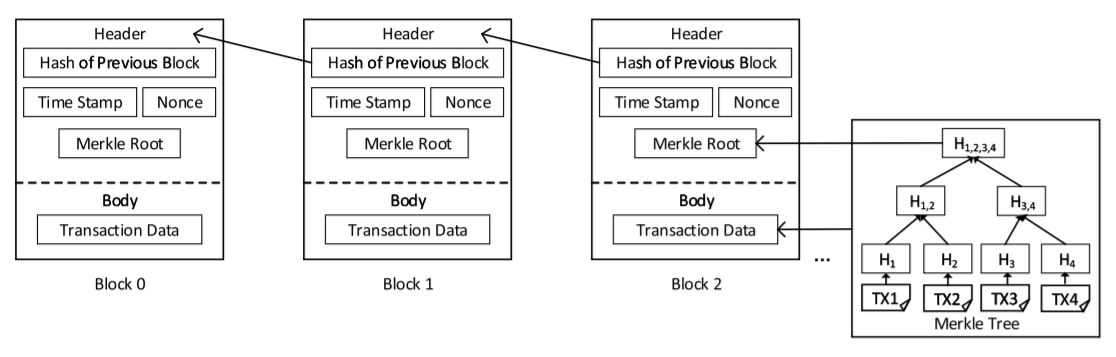
\includegraphics[width=1\textwidth, height=5cm]{gfx/figures/Block structure.JPG}
 \caption{Block Structure \cite{blockStructure}}
 \label{fig:chapter03:setup}
\end{figure}

The core components of blockchain architecture:
\begin{itemize}
    \item Node/Peer: A device (like a computer) present inside a blockchain network that has a copy of all the transactions.
    \item Transaction: It is the exchange of information between the two blockchain addresses.
    \item Block: It is used to keep a group of transactions that is distributed among all the nodes in the network.
    \item Chain: A series of blocks arranged in chronological order.
    \item Miners: Before adding any transactions to a new block node, selected nodes carry out the block verification.
    \item Consensus:  It is a mechanism through which all of the blockchain network's peers come to an agreement about any transaction in the blockchain.
\end{itemize}

\section{Evolution of blockchain}

The mainstream internet usage at the turn of the century aided the introduction of digital currency as an expansion of electronic cash systems. The following is a timeline of blockchain's growth.

\subsection{1991 - Blockchain Invention}
Scott Stornetta and Stuart Haber invented Blockchain. They created a cryptographically protected chain of blocks which would prevent anyone from tampering with document timestamps \cite{history}. 

\subsection{2008-2013 - Bitcoin Emergence}
Blockchain technology gained popularity due to Bitcoin in 2008, as it is the first application in the blockchain. Bitcoin was conceptualized by Satoshi Nakamoto. In 2009, Nakamoto published a white paper on Bitcoin. First Bitcoin was purchased for 10,000BTC in 2010. Bitcoin crosses \$1 billion in 2013.

\subsection{2013-2015 - Ethereum Development}
Ethereum was conceptualized by Vitalik Buterin. Ethereum has additional features like  smart contracts compared to Bitcoin. The development of  Ethereum has proven to be an important moment in the history of Blockchain.  Ethereum is used for cryptocurrencies and in many other decentralized applications because of smartcontracts.

 \subsection{2015 - Hyperledger}
Hyperledger was developed by Linux Foundation in 2015. It allows development of open-source blockchain. The different Hyperledger frameworks are Hyperledger Fabric, Hyperledger Iroha, Hyperledger Sawtooth, and Hyperledger Burrow \cite{hyperledgertypes}.

\subsection {2015 - Future}
Many cryptocurrencies and applications have been developed after the emergence of Bitcoin and Ethereum. Nowadays, Blockchain technology is used by various companies and organizations.

\section{Types of blockchain}

Blockchain is divided into four types, public, private, consortium and hybrid blockchains based on permission and assess.
\subsection{Public Blockchain}
It is a permissionless distributed technology. As the name suggests, anyone with the internet is allowed to access the public blockchain and participate in the transactions. Each peer in this network has their own copy of the ledger. Consensus mechanisms like \ac{PoW}, \ac{PoS}, etc., are required to reach consensus while adding new blocks and during verification of transactions. Public blockchains are fully decentralized because all the peers have equal authority, which in terms makes it secure as no one can have full control over the blockchain network. In turn,  ensuring data security helps in keeping the ledger immutable. Some examples are Bitcoin, Litecoin, and Ethereum.

Open and closed are used to tell who can read data in a blockchain. These two properties are used to describe blockchain.
\begin{itemize}
    \item Public and Open: This blockchain is accessible for everyone and data can be read by everyone. For example, cryptocurrencies like Bitcoin  and Ethereum.
    \item Public and Closed: The consumers can store confidential information and can restrict access for selected participants. In this blockchain, everyone can write in blockchain, but the reading rights are only held by selected entities. For example, Voting.
\end{itemize}


\subsection{Private Blockchain}
It is also known as permissioned blockchain. There are limitations on who can be part of the network and who can contribute to the transactions. A private blockchain is used by an organization or company for its internal usage. Private blockchains are centralized i.e, one organization has authority in the network. It provides transparency and security to the participants.
For example, Hyperledger Fabric.

\begin{itemize}
    \item Private and Open: Every contributor in the blockchain network can read the data. For example, Corporate income statements.
    
    \item Private and Closed: Only known participants can read and write in the blockchain network. For example, Tax returns, National Defense.
\end{itemize}

\subsection{Consortium Blockchain}
In this blockchain, more than one organization can manage the network, hence it is not fully centralized. It is used by organizations that need both public and private blockchain functionality. For example, Quorum and Hyperledger Fabric.


\subsection{Hybrid Blockchain}
 It is a mix of the private and public. In the blockchain, the peers determine who has access to which data. Some processes are kept private, while others are made public. On an open ledger, businesses can protect background transactions with business partners while still providing the product details to customers. For example, Dragonchain.

\section{Consensus algorithms}
All the peers have equal authority, hence it is difficult to reach consensus. Before Bitcoin, a lot of decentralized currency systems failed because when it came to reaching a consensus, they were unable to resolve the most important problem, i.e., Byzantine Generals Problem.\cite{blockchain}

\subsection{Byzantine generals problem}
The generals of various army battalions must choose whether to withdraw or assault. They must make a decision by sending messages by messengers and must reach an agreement. There's a possibility that some of the messengers and/or generals are traitors. These traitorous generals can change the message and send a malicious response, causing the loyal generals' plan to be disrupted.

\subsection{Consensus mechanisms}

The following are the few consensus mechanisms that can be used to address the issue of the Byzantine generals problem:

\subsubsection{Proof of Work} 
Bitcoin uses \ac{PoW} as the consensus mechanism. Miners “mine” a block to connect to the blockchain by solving cryptographic puzzles. This method requires a significant amount of energy and computation. The puzzles have been created in such a way that they are challenging and demanding on the system. When a miner completes the puzzle, they send their block for verification to the network. The method of determining whether a block belongs in the chain or not is extremely easy. A 51\% attack is a possible attack in the blockchain, in which a miner or a group of miners with more than 51\% of the computing power will prevent new blocks from being produced and establish false transaction records that benefit the attackers \cite{blockchain}.

\subsubsection{Proof of State}
It is a more energy-efficient version of \ac{PoW}. Nodes with the most stakes (for example, currency) are thought to be less likely to strike the network. The disadvantage here is the monopoly, when it comes to both technological and economic aspects of the scheme, the main stakeholder has full influence and authority.

\subsubsection{RAFT}
RAFT is a distributed crash fault tolerance consensus algorithm that ensures that the system can make a decision 
and process client requests in the event of a failure \cite{raft}. It is a consensus algorithm for handling a replicated log. 
Consensus in RAFT is reached through an elected leader. The server within a raft cluster is either a follower or a leader or a candidate. 
The leader is in charge of replicating logs to the followers.


\subsubsection{\ac{pBFT}}
Hyperledger fabric uses \ac{pBFT}. It is a realistic algorithm that tolerates Byzantine faults. \ac{pBFT} requires 3f+1 nodes in order to keep the system stable, where f is the maximum count of defective nodes the system can handle. As a result, approval from 2f+1 nodes is needed for the group of nodes to make any decision. Without performing complex mathematical computations (such as \ac{PoW}), \ac{pBFT} will achieve distributed consensus. Since they have been decided upon, the transactions do not need several confirmations. (For example, in Bitcoin's PoW , each node independently verifies all the transactions. Confirmations will take anywhere from 10 to 60 minutes depending on how many individuals have to confirm the new block).

\pagebreak

\section{Comparison between Hyperledger fabric and Ethereum}
\begin{table}[htbp]
\begin{center}

\begin{tabular}{ | m{3cm} | m{4.5cm}| m{4.5cm} | } 
\hline
& Hyperledger Fabric & Ethereum \\ 
\hline
Blockchain Type & Permissioned and Private & Permissionless and Private / Public\\ 
\hline
Objective & Suited for enterprises and B2B applications & Suited for B2C applications \\ 
\hline
Cryptocurrency & None & Ether \\ 
\hline
Smart contract language & JavaScript, GO and Java & Solidity \\ 
\hline
Consensus Mechanism & Pluggable consensus mechanism. Mining not required & \ac{PoW} consensus mechanism. Mining is required to reach the consensus.\\ 
\hline
Confidentiality & Confidential transactions & Transparent \\ 
\hline
\ac{tps} & > 2000 \ac{tps}  & $\approx$ 20 \ac{tps}  \\ 
\hline
\end{tabular}
\caption{Hyperledger fabric and Ethereum comparison}
\label{table:1}
    
\end{center}
\end{table}
\chapter{The Solution}
\label{ch:thesolution}

%
% Section: Scenario 
%
\section{Scenario}
\label{sec:thesolution:Scenario}

To manage the medical records of patients, need to map fabric components to requirements of the EHR systems. All hospitals act as organizations in fabric network. Patient data has been treated as assets which is stored in the ledger. It is also possible to store the reference of the EHR data in the ledger but since application is not managed by real data and for that it will be necessary to maintain the separate database which will have patients data. This can be a good solution when it is integrated with production or real hospitals EHR data. For now patient record has few fields like personal and medical details like age, address, allergies, symptoms, treatment, followup, etc. When doctor is medicating to a patient, patient history data will be available which helps doctors to assign appropriate treatment. To improve the privacy of records, it is designed to provide extra steps in application for patients. Patient can decide to have permission to access his/her data from a particular doctor. Doctor can view limited fields of assent means patient data like all medical fields along with age and allergies. Where as patient can view all the fields but edit only personal fields. 
A similar application approach also available in \cite{Dubovitskaya2020} which motivated to this solution further.

%
% Section: Why blockchain
%
\section{Why blockchain and fabric?}
\label{sec:thesolution:whyblockchain}

Blockchain has many advantages over many traditional database systems. One of the major advantages of blockchain is, it stores data cryptographically encrypted via distributed and decentralized way in peers which is nothing but a computing machine. This solves the availability of data within the network. It means for the outside world it is not possible to access data. The next benefit of blockchain is immutability. Since all the transactions are combined in a block and arranged in a chain as explained in Chapter \ref{ch:SOTA}. 

On top of the blockchain, hyperledger fabric provides some additional features which perfectly fit the current scenario. It is a permissioned and closed blockchain, no person can get added into the network unlike permissionless blockchains such as bitcoin, ethereum. This solves the confidentiality problem of patients' data. The fabric has a concept of Certificate Authority for every organization or common CA called Fabric CA and MSP which provides identities and verifies when a transaction request is made. Moreover, all the components of the fabric network are scalable and pluggable. It means more organizations can be added connected through channels, any number of peers for organizations. Like ethereum, the fabric also provides the concept of smart contracts, and when it is packaged and deployed it is called a chaincode. It is a business logic that is deployed on every endorsing peer. Initial organizations of the channel decide whether the new organizations should be added or not through Channel Configuration. It returns all the transaction information. All the components are explained further in the following section.

%
% Section: Use cases
%
\section{Use cases}
\label{sec:intro:Use cases}
There are three users in the system with role admin, patient, and doctor. Each user has its own use cases which are described in Figures \ref{fig:chapter03:admin use case}, \ref{fig:chapter03:patient use case} and \ref{fig:chapter03:doctor use case}. A user interfaces for admin from every hospital to make necessary changes about users.

\begin{figure}[htbp]
 \centering
 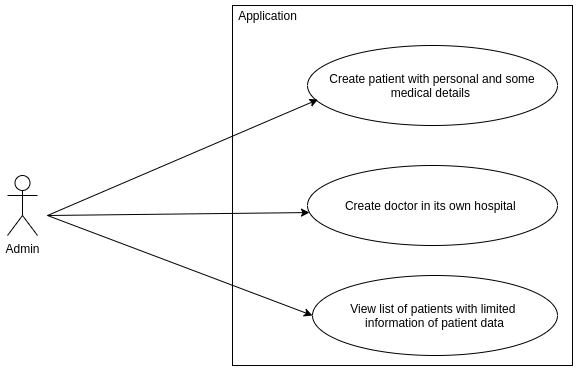
\includegraphics[width=1\textwidth, height=7cm]{gfx/figures/Admin use case .png}
 \caption{Admin use case diagram}
 \label{fig:chapter03:admin use case}
\end{figure}

\begin{figure}[htbp]
 \centering
 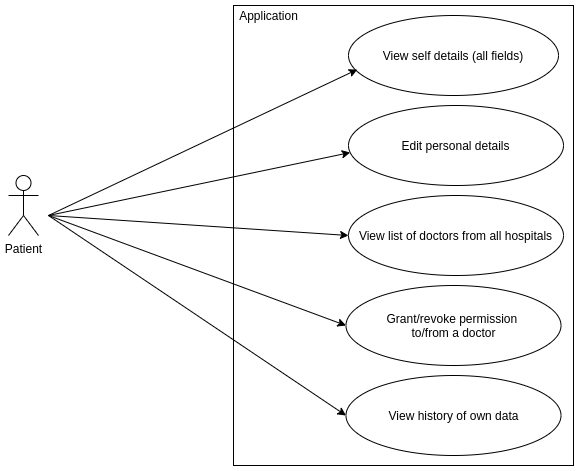
\includegraphics[width=1\textwidth, height=10cm]{gfx/figures/Patient use case.png}
 \caption{Patient Use case diagram}
 \label{fig:chapter03:patient use case}
\end{figure}

\begin{figure}[htbp]
 \centering
 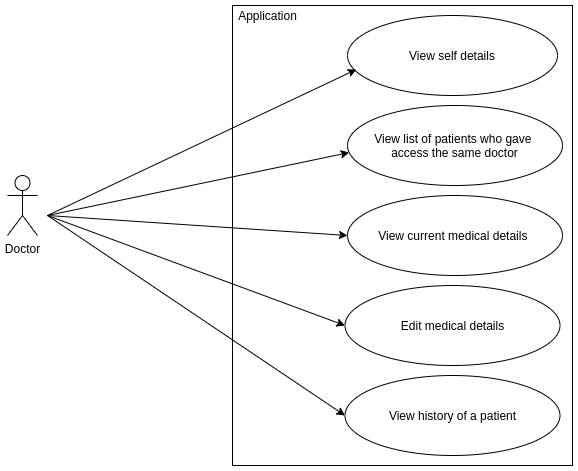
\includegraphics[width=1\textwidth, height=10cm]{gfx/figures/Doctor use case.png}
 \caption{Doctor Use case diagram}
 \label{fig:chapter03:doctor use case}
\end{figure}



%
% Section: Architecture
%
\section{Architecture}
\label{sec:implementation:architecture}

A high-level architecture of a system is depicted in Figure \ref{fig:chapter03:architecture}. The architecture also shows the fabric network in detail with color schemes. The blockchain operator setups the initial configuration of the network and provides necessary access and credentials to the users who govern the system. All the peers from the hospitals are nothing but docker containers of image hyperledger/fabric-peer, orderer, and ca. As described, every component of the application is pluggable, so backend code and smart contract are written in JavaScript language with ExpressJS as a server to provide REST API. The user interface is developed using the Angular 11 framework. The communication between the front and back end is performed through REST calls with JSON web token for authentication. Backend code can also be written in Java, Go, and Typescript which is officially supported languages by Hyperledger Fabric. For the given scenario single channel named 'hospitalChannel' and two hospital organizations are sufficient. The third hospital can also be successfully added in between when the network is running and gets joined with the same channel. 
Fabric provides support for two databases, LevelDB and CouchDB. The CouchDB is used for the solution because it is more flexible than LevelDB. Images handling is possible. It supports indexes, unlike LevelDB. Since all patient data stored in CouchDB and not maintaining any separate EHR store, CouchDB fits well. Whereas LevelDB is a powerful in-memory database developed by Google to store key-value pairs and in some cases, it is faster than CouchDB. The other use case scenario where the EHR database of hospitals is used and only stores references (maybe in the form of API) to that record in LevelDB as a blockchain ledger. Since use cases are simple here so CouchDB supports here properly. The ledger is a combination of the transaction log and world state. CouchDB is used to store the world state. Because of which no need to query the whole transaction log for every transaction request. Transaction log stores all transactions start from the first one which is stored in the genesis block. It can be found on local system at
\lstinline{/var/lib/docker/volumes/net\_peer0.org2.example.com/_data/ledgersData/chains/chains/mychannel/blockfile_000000} (depends upon the installation path). In Couchdb docker containers it is by default available at \lstinline{/var/hyperledger/production/ledgersData/chains/chains/mychannel/}. It is configurable in \href{https://github.com/kshitijyelpale/blockchain-hyperledger-fabric-electronic-patient-records/blob/main/app/first-network/docker/docker-compose-hospital-net.yaml}{docker-compose-hospital-net.yaml}. 
The Redis key-value DB is also used to store doctor credentials - username and password for doctor's credentials. Whereas other details of the doctor are stored as user attributes using fabric SDK.
The patient record has some personal and medical fields describe here in \href{https://github.com/kshitijyelpale/blockchain-hyperledger-fabric-electronic-patient-records/blob/main/app/patient-asset-transfer/chaincode/lib/initLedger.json}{initLedger} file. This is the initial data when the network gets up. Similarly, two doctors from every two hospitals are created.


\begin{figure}[htbp]
 \centering
 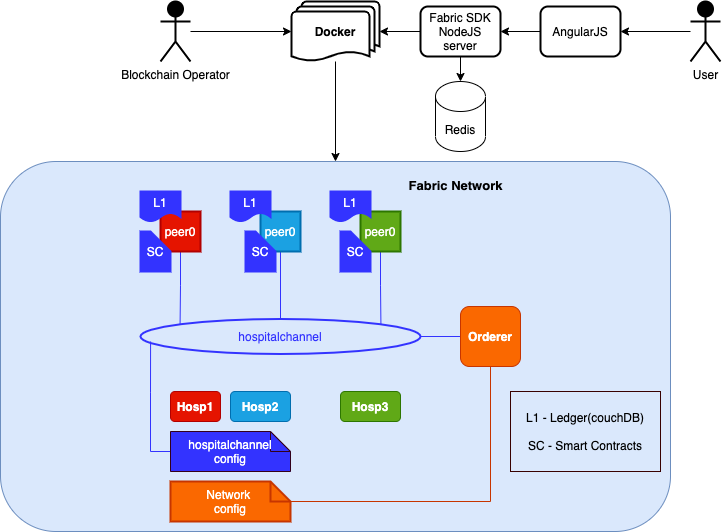
\includegraphics[width=1\textwidth, height=10cm]{gfx/figures/Architecture.png}
 \caption{Architecture}
 \label{fig:chapter03:architecture}
\end{figure}

% Section: Network/activity diagram
%
\section{Activity diagram}
\label{sec:thesolution:network/acitivitydiagram}

The Figure \ref{fig:chapter03:activityFirst} shows the interaction between components for creation of a patient. The patient needs to create an account only the first time the patient visits any one of the hospitals in the network, during the first visit the patient provides details to the admin, admin invokes the \lstinline{AdminContract} to create a patient. In the backend, firstly the admin certificate is used to connect to the network, and a transaction is created which adds the patient object to the ledger and also adds the patient identity to the blockchain network. After the creation of the patient is successful, the server creates a temporary password for the patient using which the patient can log in to the network. The patient credentials are added to the ledger as the patient can go to any of the hospitals in the network. The Figure \ref{fig:chapter03:activitySecond} shows the interaction to create a doctor. The doctor provides details to the admin, who then firstly connects to the network and then adds the doctor as an identity to the blockchain network. And the credentials of the doctor are stored in the hospital-specific Redis database. Now as patient and doctor are added as identities in the blockchain network, for the next interaction the patient/doctor can connect to the network using their certificates.

\begin{figure}[htbp]
 \centering
 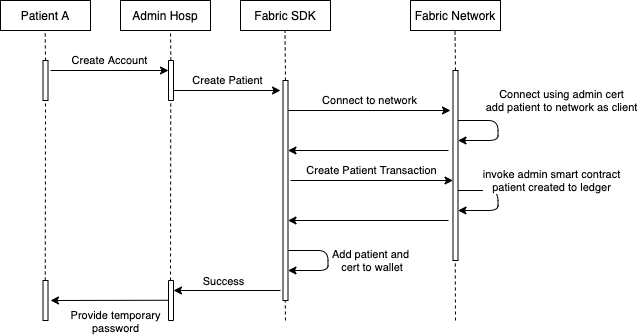
\includegraphics[height=6cm]{gfx/figures/first.png}
 \caption{Creation of a patient}
 \label{fig:chapter03:activityFirst}
\end{figure}

\begin{figure}[htbp]
 \centering
 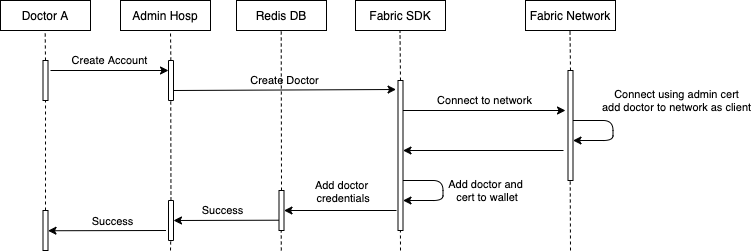
\includegraphics[height=5cm]{gfx/figures/second.png}
 \caption{Creation of a doctor}
 \label{fig:chapter03:activitySecond}
\end{figure}


\section{Applying Fabric Components}
\label{sec:thesolution:fabriccomponents}
The HLF comprises many components, has a complex architecture. And these components can be applied and used in many various ways. The following describes how HLF components are applied.

\subsection{Smart Contract \& Chaincode}
A smart contract in hyperledger fabric defines the transaction logic that controls the lifecycle of a business object contained in the world state \cite{Smart-Contracts-Chaincode}. Mutiple Smart contracts are packaged into a single chaincode which is then deployed to a blockchain network. A smart contract defines the rules between different organizations in executable code. Fabric SDK invokes a smart contract to create transactions which then performs changes to the ledger. A smart contract is defined within a chaincode. Multiple smart contracts can be defined within the same chaincode. When a chaincode is deployed, all smart contracts within it are made available to applications.
As shown in Figure \ref{fig:chapter03:smartContractHierarchy} the application comprises mainly three smart contracts packaged into a single chaincode - each role (Patient/Doctor/Admin) invokes its very own smart contract.
\begin{itemize}
    \item \lstinline{AdminContract} - This contract is invoked by the admin. The methods in the contract give the admin the ability to create/delete patients by adding/deleting patient object to from the ledger. Admin can also view all the patients available throughout the network. 
    \item \lstinline{PatientContract} - The patient interacts with the ledger by invoking this contract. The contract contains the logic that is required for the patient. For instance, only the patient can update/view the personal details and password via the methods defined in the contract. And also patient contract contains methods to grant and revoke access to from a doctor. 
    \item \lstinline{DoctorContract} - The doctor contract has methods that allows the doctor to update/read the patients medical details. 
\end{itemize}
The idealogy for the three smart contracts is to make sure that the right role has the right access to the data on the ledger. Only the patient has the right to update the personal details, grant/revoke access, and update the password. These methods can be invoked by neither the admin nor the doctor. And similarly, the methods of the doctor cannot be accessed by the patient or admin. The read patient method is common for all, but the data which is retrieved by the contract is different for each role admin just has the access to patient name, the doctor has the access to the medical details and the patient has the access to the whole object. 

\begin{figure}[htbp]
 \centering
 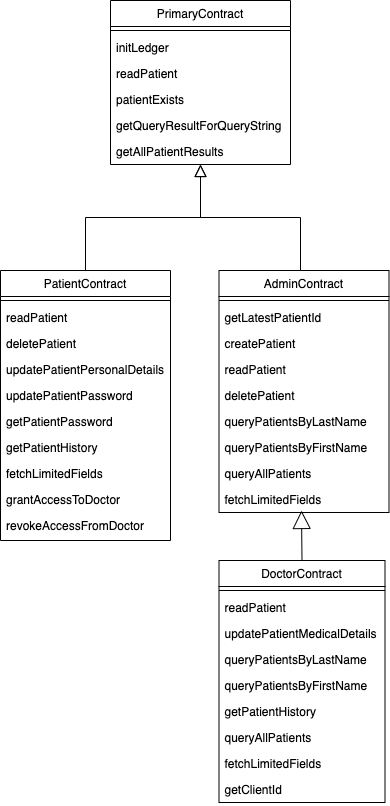
\includegraphics[width=6cm, height=10cm]{gfx/figures/smartContractHierarchy.png}
 \caption{Smart Contracts Hierarchy}
 \label{fig:chapter03:smartContractHierarchy}
\end{figure}

\subsection{Endorsement policies}
The chaincodes in Hyperledger fabric have an endorsement policy that specifies the peers on the channel that executes the chaincode functions and endorses the results to the ledger and makes the transaction valid. The endorsement policies define the peers which will verify and approve/reject the execution of a transaction. During this process, the peers verify the transaction, and the committing peer ensures sure that the transaction contains the the required number of endorsements which is configured in the endorsement policy.\cite{Policies}.

The Endorsement Policy is defined in the \href{https://github.com/kshitijyelpale/blockchain-hyperledger-fabric-electronic-patient-records/blob/main/app/first-network/configtx/configtx.yaml}{configtx.yaml}. Each hospital contains its very own endorsing peers as specified in the YAML file in the path \lstinline{&hosp1/Policies/Endorsement} similarly for hosp2. The rule specifies the roles who are endorsers. In the YAML file, all the peers of the hospitals are endorsers. A Chaincode-level endorsement policy is defined in the YAML file in the PATH Application: \lstinline{&ApplicationDefaults/Policies/Endorsement} \lstinline{`MAJORITY`} specifies that only when a majority of channel members approve a chaincode definition then definition iscommitted to the channel.

\subsection{Endorsing members of hospitals}
In path \lstinline{&hosp1/Policies/Endorsement} the rule \lstinline{OR('hosp1MSP.peer')}  requests one signature from the peers of hosp1. Other values can be : \\ 
\begin{itemize}
    \item Requests one signature from each role 
        \begin{lstlisting}
            AND('hosp1MSP.peer', 'hosp1MSP.admin')
        \end{lstlisting} 
    \item Requests one signature from either one of the roles 
        \begin{lstlisting}
            OR('hosp1MSP.peer', 'hosp1MSP.admin') 
        \end{lstlisting} 
\end{itemize}

\subsection{Specifying the endorsing policy}
In path \lstinline{&ApplicationDefaults/Policies/Endorsement} other types can be a signature with the one of the following rules:
\begin{itemize}
    \item A transaction is commited only if admin of the both the hospital approve.
        \begin{lstlisting}
            AND('hosp1MSP.admin', 'hosp2MSP.admin') 
        \end{lstlisting} 
    \item A transaction is commited only if either one of the admin of the both the hospital approve. 
        \begin{lstlisting}
            OR('hosp1MSP.admin', 'hosp2MSP.admin')
        \end{lstlisting} 
    \item \lstinline{OutOf(1, 'hosp1MSP.admin', 'hosp2MSP.admin')} which is equivalent to \lstinline{OR('hosp1MSP.admin', 'hosp2MSP.admin')}
\end{itemize}

\subsection{Ledger}
A Distributed ledger in Hyperledger Fabric as shown in Figure \ref{fig:chapter03:ledger} - one that is logically singular, but has many consistent copies distributed throughout a network comprises of two parts - the world state which holds the current values of the objects, the other part is the blockchain which is the history of the transactions which resulted to the current world state\cite{Ledger}.

\begin{figure}[htbp]
 \centering
 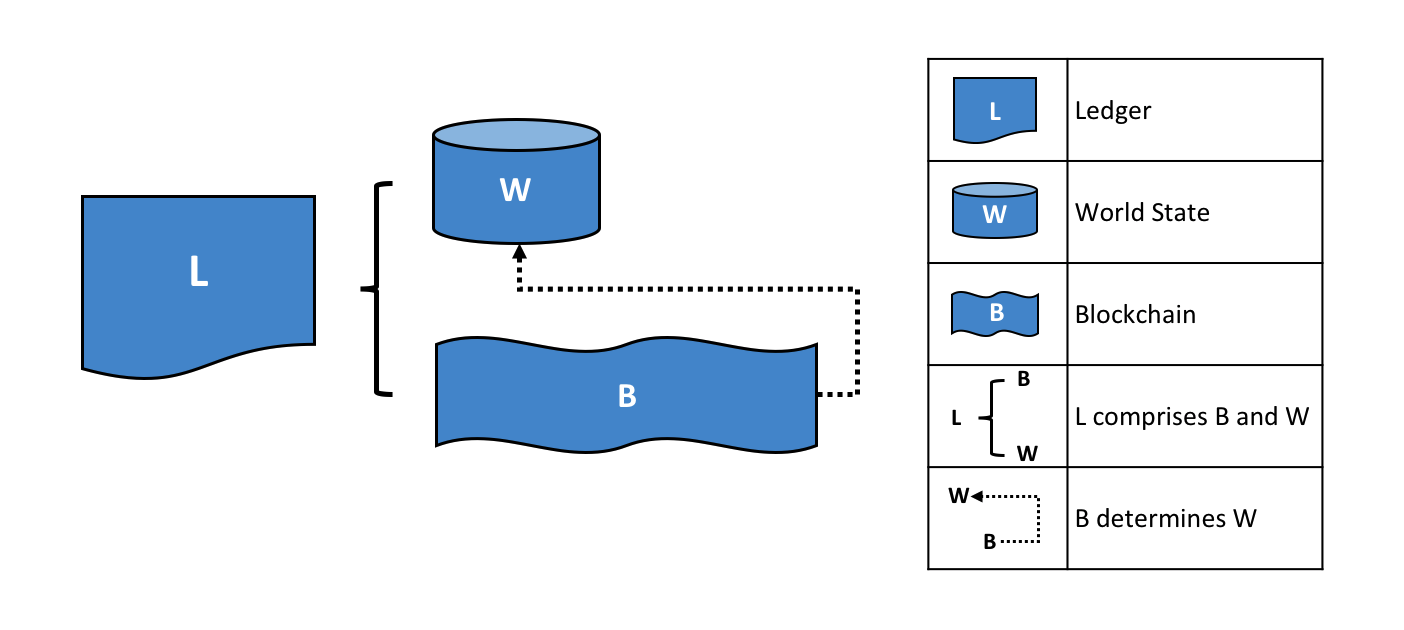
\includegraphics[width=10cm, height=6cm]{gfx/figures/ledger.diagram.1.png}
 \caption{Ledger in Hyperledger Fabric \cite{Ledger}}
 \label{fig:chapter03:ledger}
\end{figure}

In the application, the idealogy of a ledger can be thought of as one logical database in a Hyperledger Fabric network. In reality, the network contains multiple copies of a ledger for each hospital's peers – which are kept consistent with every other copy through consensus. The ledger in the application is being utilized in the following ways 
\begin{itemize}
    \item Firstly, the world state is the database where all the patient data is stored. All patients that are queried and updated are stored in the world state. All the query transactions are retrieved from the world state.
    \item Secondly, the transaction log which is a sequential structured interlinked blocks of log files, where each block contains a sequence of transactions, and a transaction represents a query or an update to the world state. The getHistory API specifically  uses the  transaction log to retrieve the history of an asset.
\end{itemize}

\subsection{Identity (CA)}
For a participant of a hospital, the participants first need to prove that can be are trusted to make transactions in the blockchain network. An identity for each participant issued by a trusted authority is required to be recognized in this network \cite{Identity}. The MSPs are the trusted authorities - which can be found in \href{https://github.com/kshitijyelpale/blockchain-hyperledger-fabric-electronic-patient-records/blob/main/app/first-network/configtx/configtx.yaml}{configtx.yaml}. An Hospital Certificate Authority(CA) dispenses certificates to each of its participants. These certificates are digitally signed by the CA and bind together the participant with the participant’s public key with a set of permissions. As a result, if one trusts the CA (and knows its public key), it can trust that the specific participant bound to the public key included in the certificate by validating the CA’s signature on the participant’s certificate. In the application either CAs(default) or cryptogen can be used to issue identities in the network: 
\begin{itemize}
    \item \emph{Cryptogen}: Cryptogen is a tool that creates certificates and keys. This tool can be used during development and testing. The tool quickly just creates the required crypto material for the hospitals\cite{Cryptogen}. The configuration files for all the hospitals and the orderer are defined in \href{https://github.com/kshitijyelpale/blockchain-hyperledger-fabric-electronic-patient-records/tree/main/app/first-network/organizations/cryptogen}{cryptogen} directory, the \lstinline{YAML} files contain the necessary information for the tool to create the cryto material for the hospitals and the Orderer.
    \item \emph{CAs}: Each hospital has its very own CA server that creates the identities using client of the server to prove that the identity belong to their hospital and can be trsuted. All of the identities created by a CA run of the hospital share the same trust of the root CA \cite{Identity}. The application uses CAs to allows registration and enrolling patients/doctors with the Fabric SDK which cannot be done using Cryptogen. The configuration files of the CAs of the hospitals and orderer defined in \href{https://github.com/kshitijyelpale/blockchain-hyperledger-fabric-electronic-patient-records/blob/main/app/first-network/organizations/fabric-ca/hosp1/fabric-ca-server-config.yaml}{Hosp1CA}, \href{https://github.com/kshitijyelpale/blockchain-hyperledger-fabric-electronic-patient-records/blob/main/app/first-network/organizations/fabric-ca/hosp2/fabric-ca-server-config.yaml}{Hosp2CA} and \href{https://github.com/kshitijyelpale/blockchain-hyperledger-fabric-electronic-patient-records/blob/main/app/first-network/organizations/fabric-ca/ordererOrg/fabric-ca-server-config.yaml}{OrdererCA} respectively. 
\end{itemize}


\subsection{Membership Service Provider (MSP)}
Hyperledger Fabric is a permissioned blockchain network, all the participants of the network, in our application the peers/doctors/patients need to prove their identity to join and perform transactions in the blockchain network to prove that these participants can be trusted. Hyperledger Fabric uses a Public Key Infrastructure (PKI) \cite{MSP} to verify identities in a chain of trust. The fabric uses Certificate Authorities(CA) to prove identity, the CAs generate a public and a private key for each identity which forms a key-pair using which the participants can prove their identity and be recognized in the network. The MSP is the one that verifies the private keys of the participants by matching them with the stored public key. For instance, in the application the peers of the hospital endorse a transaction using its private key, the MSP on the ordering service is where the public key is stored which is used to verify that the private key attached to the transaction is valid. CAs are used to create trusted identities that are recognized by the network(peers/doctors/patients). MSPs are used for defining the hospitals that are trusted by the network members. MSPs are allocated the participants of the hospitals with a set of roles and permissions within the network. In the applications, all the hospitals that join the network can perform read/write transactions in the network. These permissions are configured in \href{https://github.com/kshitijyelpale/blockchain-hyperledger-fabric-electronic-patient-records/blob/main/app/first-network/configtx/configtx.yaml}{configtx.yaml} and for participants of these hospitals to perform a transaction in the network they first have to have an identity issued by a CA that is recognized in the network. And be a member of any of the hospitals - MSP is how the participants are linked as a member to the hospital, this is when the public key of the participant is stored in the hospital MSP.

%
% Section: Security Mechanisms
%
\section{Security Mechanisms}
\label{sec:thesolution:securitymechanisms}
Security of the data is essential when question arises for patient data in medical data. Blockchain concept is very safe and secure itself and provides a mechanism of chaining in which if any transaction changes all successive blocks needs to change which is a very heavy task. In addition to that in hyperledger fabric when new peer and or organizations joins the channel approved by in channel configuration, still it should not be exposed, as it is available for all kind of peers. To avoid that data can be encrypted or hidden based on patient's grant/revoke actions for doctors. The proof of concepts of two mechanisms are described further. Unfortunately it is not yet implemented due to some unavoidable reasons. 

\subsection{Private Collections}
The data used and stored in Healthcare is highly confidential and must be secure. The data of the patient must be private to only the hospitals or doctors that the patient has allowed access to. Hyperledger Fabric contains functionality to store private data using private data collections\cite{Privatedata}. Private data is the data that must be kept private from other hospitals or doctors. A private data collection contains two elements:
\begin{itemize}
    \item \emph{The actual private data}: Only the data of the private collections that are authorized for particular hospitals can be accessed. 
    \item \emph{A hash of that data}: Patient data for which the hospital does not have the authorization, this data is hashed and stored and cannot be accessed by the member of the hospital.
\end{itemize}
In this application, there are n! + 1 number of private data collections where n is the number of hospitals. For instance, if there are 3 hospitals, there will be 7 private data collections. There will be a private data collection for each combination such as there will be a private collection for each hospital and a private collection which will be shared by any two hospitals and one private data collection shared by all the hospitals. The patient data stored on the collection depends on the doctors to which patient has authorized. If the patient has authorized to only one hospital, this will be stored in the private collection of that hospital. Now if the patient grants access to a doctor of another hospital, the private data is moved from the current collections to the collection which is private to the two hospitals. There will be no duplicate of the data. The patient data will always be in any one of the private data collection. The same mechanisms are applied when the patient revokes access from a hospital.

\subsubsection{Implementation Example}

Let us consider if there are two hospitals named Hospital 1 and Hospital 2. There will be a total of 3 private data collections named \lstinline{Hosp1PrivateCollection} which contains patient data which is authorized only for Hospital 1 similar \lstinline{Hosp2PrivateCollection} and a collection named \lstinline{Hosp12PrivateCollection} which is private to both Hospital 1 and Hospital 2, in this collection the patient would have granted access to both the hospitals. The channel world state will contain the assedId and the collection in which the asset is stored. This makes the reading of the patient data faster. 

\subsubsection{Scenarios}
\begin{itemize}
    \item \emph{Read/Update Patient}: First the patientId is read on the world state which will give the private data collection name, and then the patient data is read/updated from that private collecion.
    \item \emph{Grant/Revoke access to a new Hospital}: For instance if a patient is present in \lstinline{Hosp1PrivateCollection} and this patient grants access to Hospital 2, The data is first copied into \lstinline{Hosp12PrivateCollection} and then deleted in \lstinline{Hosp1PrivateCollection}.
    \item \emph{Get History}: The private data collections has not been implemented yet in the application due to the work in progress.Read the section for more details in Chapter \ref{sec:results:issues:getHistoryForKey}
\end{itemize}

\begin{figure}[htbp]
 \centering
 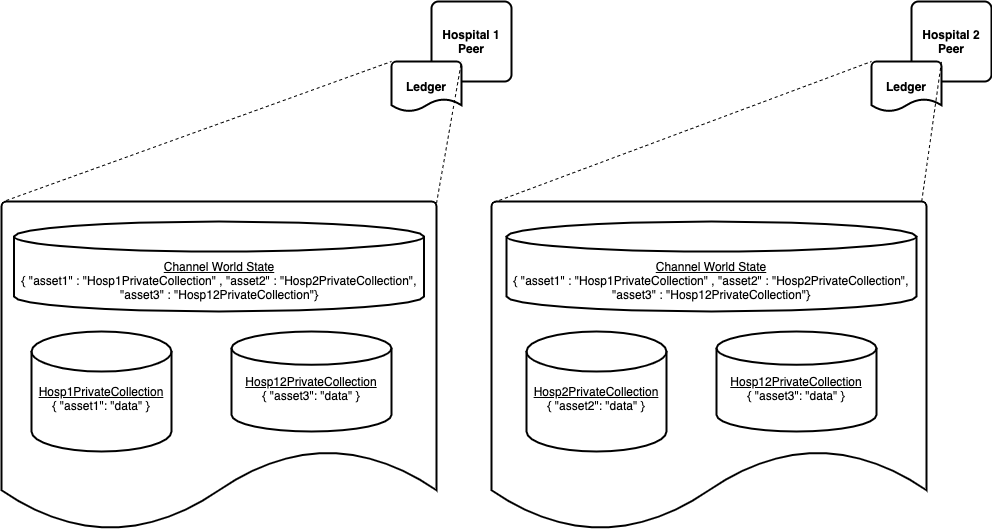
\includegraphics[width=1\textwidth, height=6cm]{gfx/figures/PrivateChannel.png}
 \caption{Private Data Collections}
 \label{fig:chapter03:privateCollection}
\end{figure}

\subsection{Data re-encryption}

It is a very common technique to store data in an encrypted format and decrypt it whenever is required. There are two types of encryption - Symmetric and asymmetric encryption. In the symmetric encryption technique, a common key is used to encrypt and decrypt the data. Whereas two different keys are used in asymmetric cryptographic encryption methods which are called private and public keys. It is also called public-key cryptography. RSA (Rivest–Shamir–Adleman) is a common algorithm used by modern computers to encrypt and decrypt data. 
typical use case, user A sends data to user B by encrypting data using user B's public key. Public keys are publically available for usage. To prove the authenticity of a public key, it is signed by some authority using a digital signature. Certificate Authority is an entity that issues a digital certificate. A digital certificate certifies the ownership of a public key of a user or an organization. So when user B receives data, it is decrypted by its private key. In the reverse mechanism, i.e., data encrypted by a private key and decrypted by the public key used in case of authentication a user.


\begin{figure}[htbp]
 \centering
 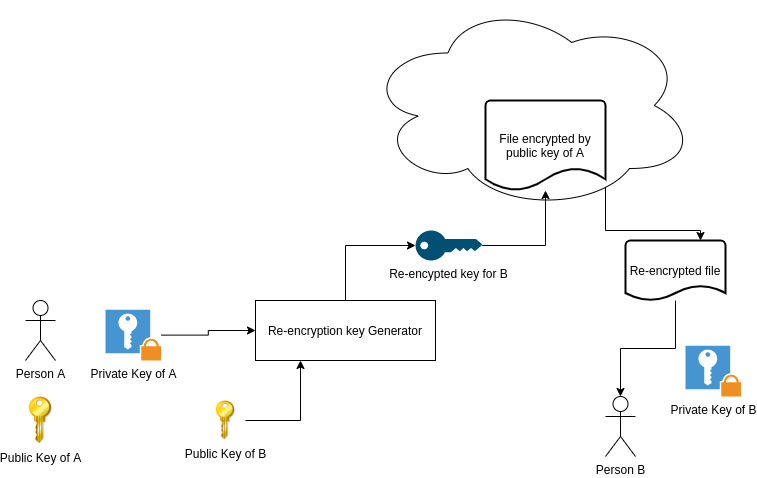
\includegraphics[width=1\textwidth, height=8cm]{gfx/figures/Re-encryption.png}
 \caption{Re-encryption}
 \label{fig:chapter03:reencryption}
\end{figure}

Consider the scenario depicted in Figure \ref{fig:chapter03:reencryption}. Person A has a data file on the cloud and person B wants to access the data. So typically, person A has to download the file, encrypt it with person B's public key, and then person B can decrypt it with its private key. These steps have some limitations. Person A needs to download the file and do encryption which is not feasible as the file size can be large and after encryption person needs to upload. So in the re-encryption approach, person A generates a re-encryption key from its private key and person B's public key, so it is a combination. This key sends to person B and the person re-encrypts the cloud file. The file is already encrypted by person A's public key but it encrypts again with the re-encryption key so the name is that way. After re-encryption, person B decrypts the file using its private key \cite{Tith2020}. Now even if the re-encryption key is lost or someones else found it, still at the end it needs to be decrypted by person B's private key. So it is secure.
The same approach can be applied in this scenario. The patient record would look as follows:

\begin{lstlisting}[language=json,firstnumber=1]
{
"patientId": "p1",
"password": hash(pwd),
"pwdTemp": true
"firstName": "abc",
"lastName" "xyz",
"data": encrypted patient data using symmetric key,
"changedBy": "doctorId XX",
"permissionGranted": [doctorId1: re-encrypted key for doctor 1, doctorId2: re-encrypted key for doctor 2, ...],
"encryptedSymmetricKey" : "######"
}    
\end{lstlisting}

All personal and medical fields are encrypted by some randomly generated key which is used as a symmetric key and stored in data as shown above. The symmetric key is also encrypted by the patient's public key and stored in the ledger under 'encryptedSymmetricKey' field. The reason behind using both encryption methods is, that a symmetric key is mostly recommended to encrypt large data. So when a patient provides access to a doctor then the re-encrypted key is calculated and stored with doctorId in the 'permissionGranted' field. So that when the doctor reads the ledger, if that doctorId is present then that re-encrypted key can be used to re-encrypt the 'encryptedSymmetricKey' and then decrypt using the doctor's private key. Once a doctor gets a symmetric key then it can easily be used to decrypt data. So basically data is encrypted only by symmetric but a re-encryption mechanism is applied to hide the symmetric key so it makes the mechanism quite robust. 


\chapter{Implementation}
\label{ch:implementation}

\section{Fabric SDK}
\label{sec:implementation:sdk}
The Hyperledger Fabric Client SDK provides APIs to interact with the Hyperledger Fabric blockchain, for instance, provides APIs to interact with smart contracts, submit transactions to a ledger, and query the ledger \cite{fabric-sdk-node}. The Fabric SDK provides the following packages:
\begin{itemize}
    \item \lstinline{fabric-ca-client} - The fabric-ca provides APIs to register and to enroll participants(admin/patient/doctor) to establish trusted identities on the blockchain network. The package creates a new CA client for interacting with the CA server of the hospital to register and enroll the participants. 
    \item \lstinline{fabric-common} - encapsulates the common code used by all fabric-sdk-node packages supporting fine-grain interactions with the Fabric network to send transaction invocations. Provides APIs to monitoring events, logging and configuration settings of the environment variable, program arguments, in-memory settings
    \item \lstinline{fabric-network} - This package contains the APIs required to connect to the Fabric network, submit transactions to query or edit  the ledger. Provides APIs to manage the wallet which is used for managing identities and create a connection profile based on the \href{https://github.com/kshitijyelpale/blockchain-hyperledger-fabric-electronic-patient-records/blob/main/app/first-network/organizations/ccp-template.json}{connection profile JSON} generated when CA is created.
\end{itemize}
In package fabric-network - The main class that allows the Fabric SDK to interact with the network is the Gateway class. Once instantiated, the object create a gateway/connection to a peer/user within the blockchain network and enables access to the chaincode and channels for which that peer/user is a member.  \cite{fabric-sdk-node}.



%
% Section: Steps to use the application 
%
\section{Steps to use the application}
\label{sec:implementation:steps}
This section describes very detailed steps to run the application start from the prerequisites. The project is available on \href{https://github.com/kshitijyelpale/blockchain-hyperledger-fabric-electronic-patient-records}{GitHub} 

\subsection{Prerequisites}
The system should have installed some tools such as docker, docker-compose, node, npm, golang, curl. Follow the detailed steps on the official website of fabric for the specific version and commands \cite{prerequisites}.

Download the fabric basic framework which generates platform-specific binaries and Docker images \cite{download-fabric-samples}.
Execute the following curl command.

\lstinline{curl -sSL https://bit.ly/2ysbOFE | bash -s -- 2.2.2 1.4.9}

This generates all test network code in folder 'fabric samples'. Now clone this project's git repository. Copy bin directory from 'fabric samples' to
\lstinline{blockchain-hyperledger-fabric-electronic-patient-records/app}.

\subsection{Start network}
\label{sec:implementation:steps:startnetwork}

Go to the first network directory and execute the network.sh file with argument up. 

\lstinline{./network up} 

This command brings up all docker containers required for two hospital organizations.

\lstinline{./network createChannel} 

This command creates a channel 'hospitalChannel' on which both organizations are connected.

\lstinline{./network deployCC} 

This command packages the smart contract code inside 'patient-asset-transfer'. The initial data of six patients are created in a ledger 
The folder structure looks similar to fabric samples which helps a developer who is already worked with the test network. 

\subsection{Add additional hospital}
\label{sec:implementation:steps:additionalhospital}

In addition to the existing two hospital organizations, one can also add a new hospital organization called hosp3. Go inside 'addHosp3' of the first-network directory.

\lstinline{./addHosp3 up}

This command brings up the containers required for hospital3 to work and join 'hospitalChannel'. If there are multiple channels in the network, it is mandatory to specify which channel to connect to. 

\lstinline{./addHosp3 deployCC} 

This command installs chaincode on hosp3 nodes. Hosp3 added separately to show that framework provides pluggable architecture. On scaling the network, new organizations can be easily added without down the existing network. Still, this solution is needed to be improved to support this pluggable feature more mature. Few things are hardcoded in the backend and front end.

\subsection{Bring up the backend and frontend}
\label{sec:implementation:steps:bringupbackend}

Go to app/server. 

\lstinline{npm install} 

This command installs all dependency files required for the backend server to run.

\lstinline{npm start} 

This command starts the express js backend server. It also enrolls and registers few users from the network. It includes both admin users from hospital organizations, initial six patient data, and four doctors. The users are created inside the wallet.  
Now go to app/client

\lstinline{npm install} 

\lstinline{ng serve -o} 

This brings up the angular server and automatically opened up in the default browser.   

%
% Section: Screenshots  
%
\section{Workflow} 
\label{sec:implementation:screenshots}

This section describes the working of the application through the perspective of all users - admin, patient, and doctor.

\subsection{Login Admin}
An admin is created for each hospital that joins the network. The details of the admin must be present during the addition of the hospital to the network. The admin details (username and password) are present in the fabric-ca-server-config.yaml of the respective hospital CA configuration. The login page for the admin is as shown in Figure \ref{fig:chapter03:admin1} the role admin has to be chosen, as the web application is the same for all the participants, the admin must choose the hospital and enter the credentials. These credentials are checked against the credentials stored in the blockchain network which was configured in the Hospital CA config YAML file.
\begin{figure}[htbp]
 \centering
 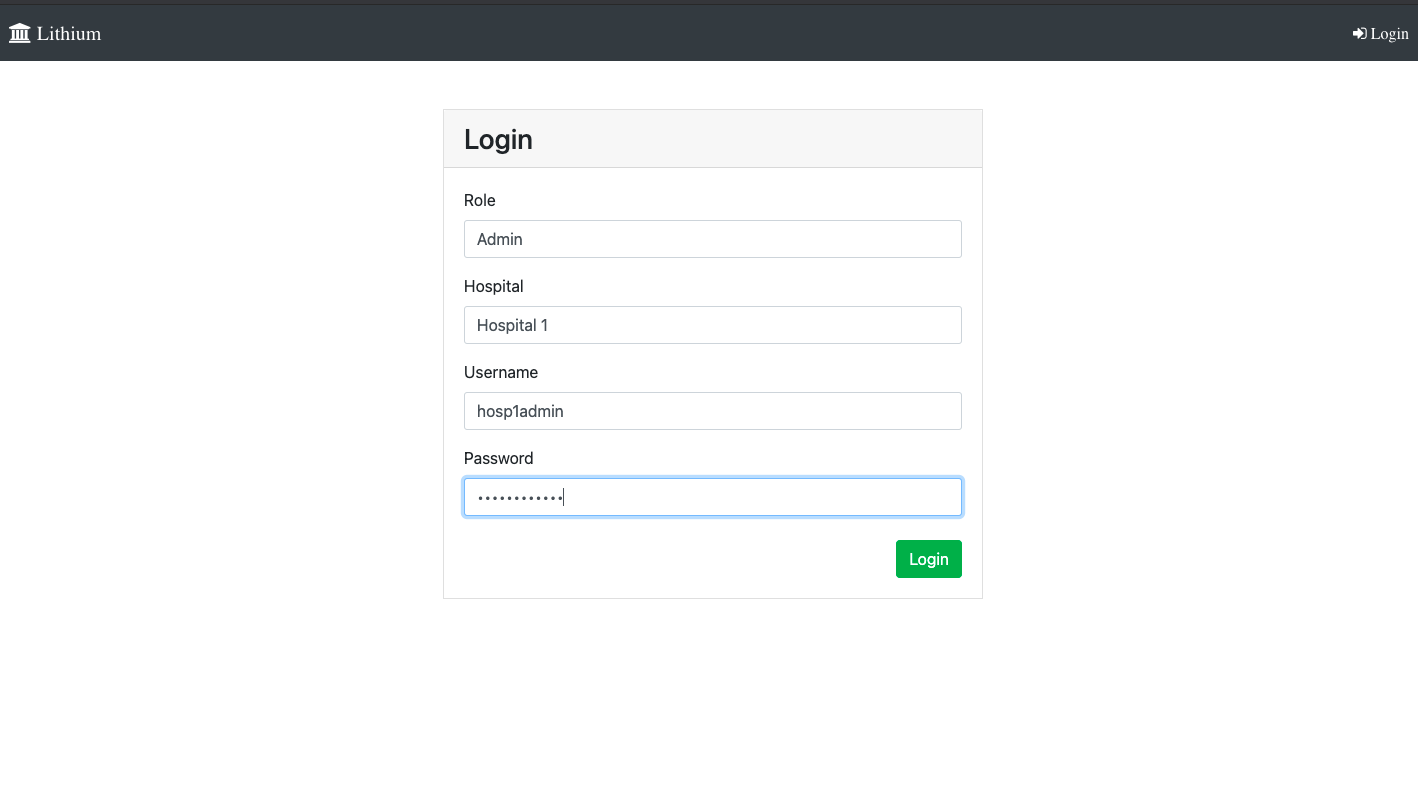
\includegraphics[height=8cm]{gfx/figures/admin1.png}
 \caption{Admin Loogin Screen}
 \label{fig:chapter03:admin1}
\end{figure}

\subsection{Admin Dashboard}
As soon the admin log in successfully, a dashboard is displayed which contains the list of all the patients in the network and the functions highlighted in Figure \ref{fig:chapter03:admin2}. The patient list is retrieved by invoking the admin contract through which a transaction is created in the ledger to retrieve all the patient objects in the world state. The admin has access only to the names of the patient other details are restricted by the contract.
\begin{figure}[htbp]
 \centering
 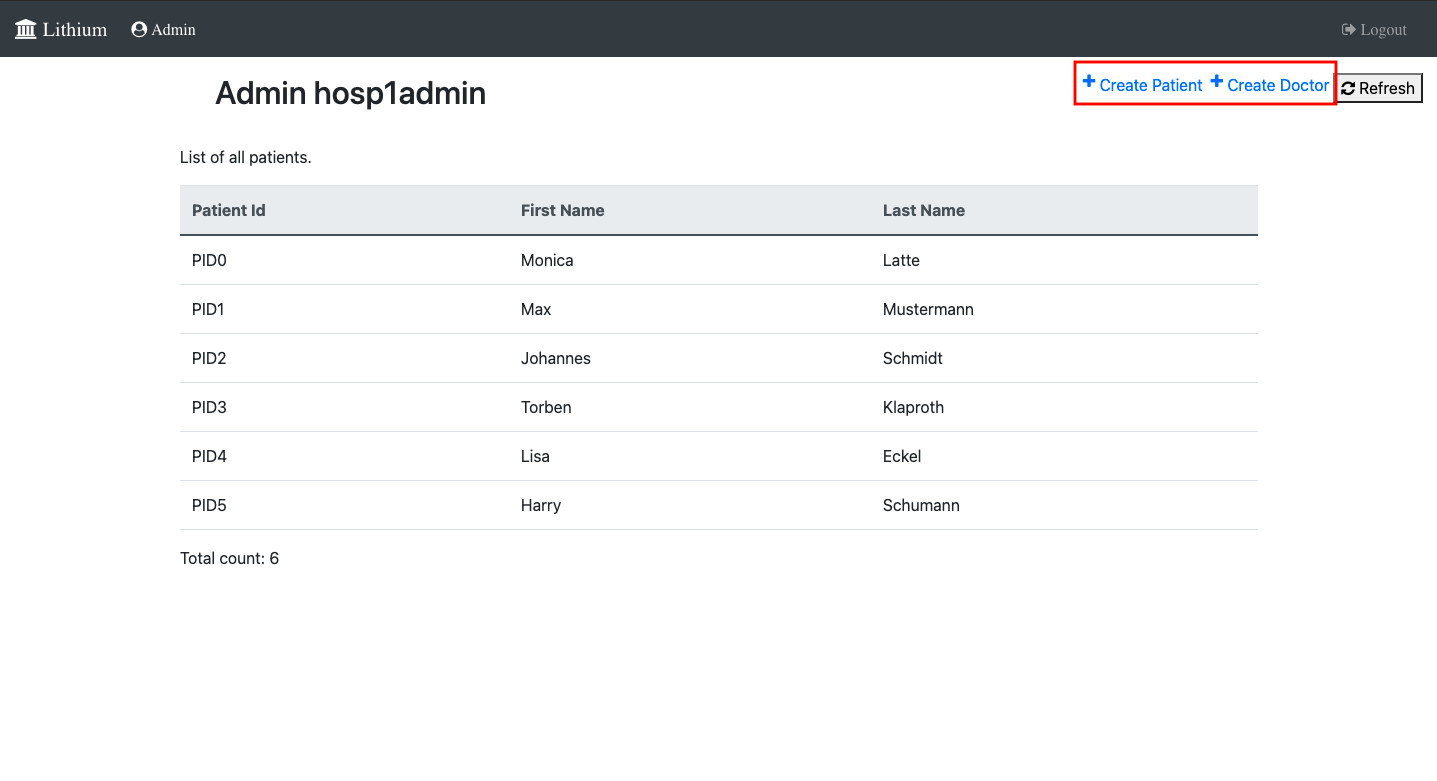
\includegraphics[height=8cm]{gfx/figures/admin2.png}
 \caption{Admin Dashboard}
 \label{fig:chapter03:admin2}
\end{figure}

\subsection{Create Patient}
The admin has the capability to create a patient that is creating a transaction in the ledger to create an object to the world state. The admin must enter the basic info of the patient as shown in Figure \ref{fig:chapter03:admin4} on save a transaction is created in the ledger and sent to all the peers of the network. The patient data is validated and if valid endorsed and stored in the ledger. The patient is also created as a client in the network using this client the patient can interact with the ledger. And on save, temporary patient credentials are created, which the patient must change on the first login for security reasons. Figure \ref{fig:chapter03:admin5} shows the list of all patients, the created patient was added to the ledger and hence is retrieved when all the patients are queried again.
\begin{figure}[htbp]
 \centering
 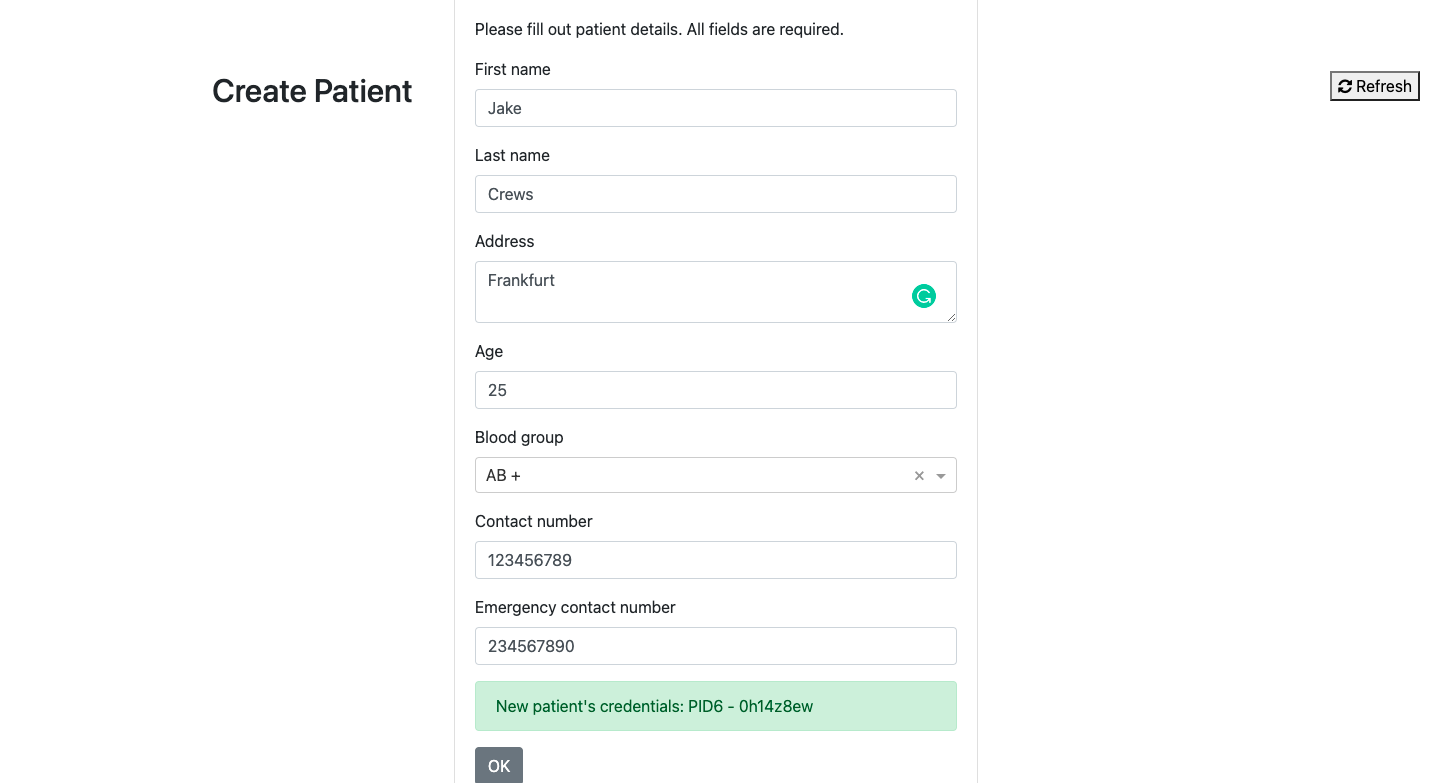
\includegraphics[height=8cm]{gfx/figures/admin4.png}
 \caption{Create Patient}
 \label{fig:chapter03:admin4}
\end{figure}
\begin{figure}[htbp]
 \centering
 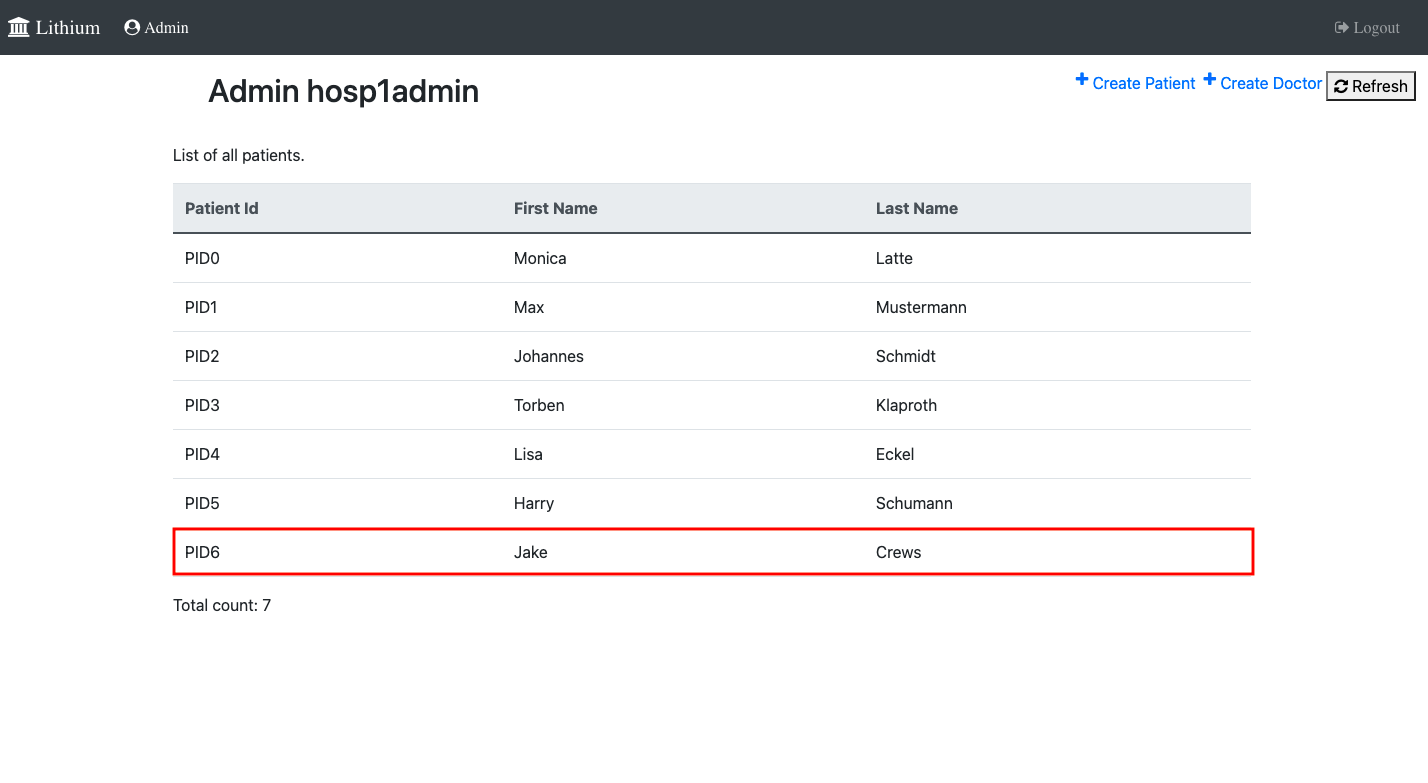
\includegraphics[height=8cm]{gfx/figures/admin5.png}
 \caption{Admin Dashboard}
 \label{fig:chapter03:admin5}
\end{figure}

\subsection{Create Doctor}
The admin can also create a doctor. As the doctor is not an object that is stored in the ledger, a client is created in the network using which the doctor now can interact with the ledger. There is no interaction with the ledger on the creation of the doctor. The admin must enter the details of the doctor as shown in Figure \ref{fig:chapter03:admin6} and on save a client is created in the network.
\begin{figure}[htbp]
 \centering
 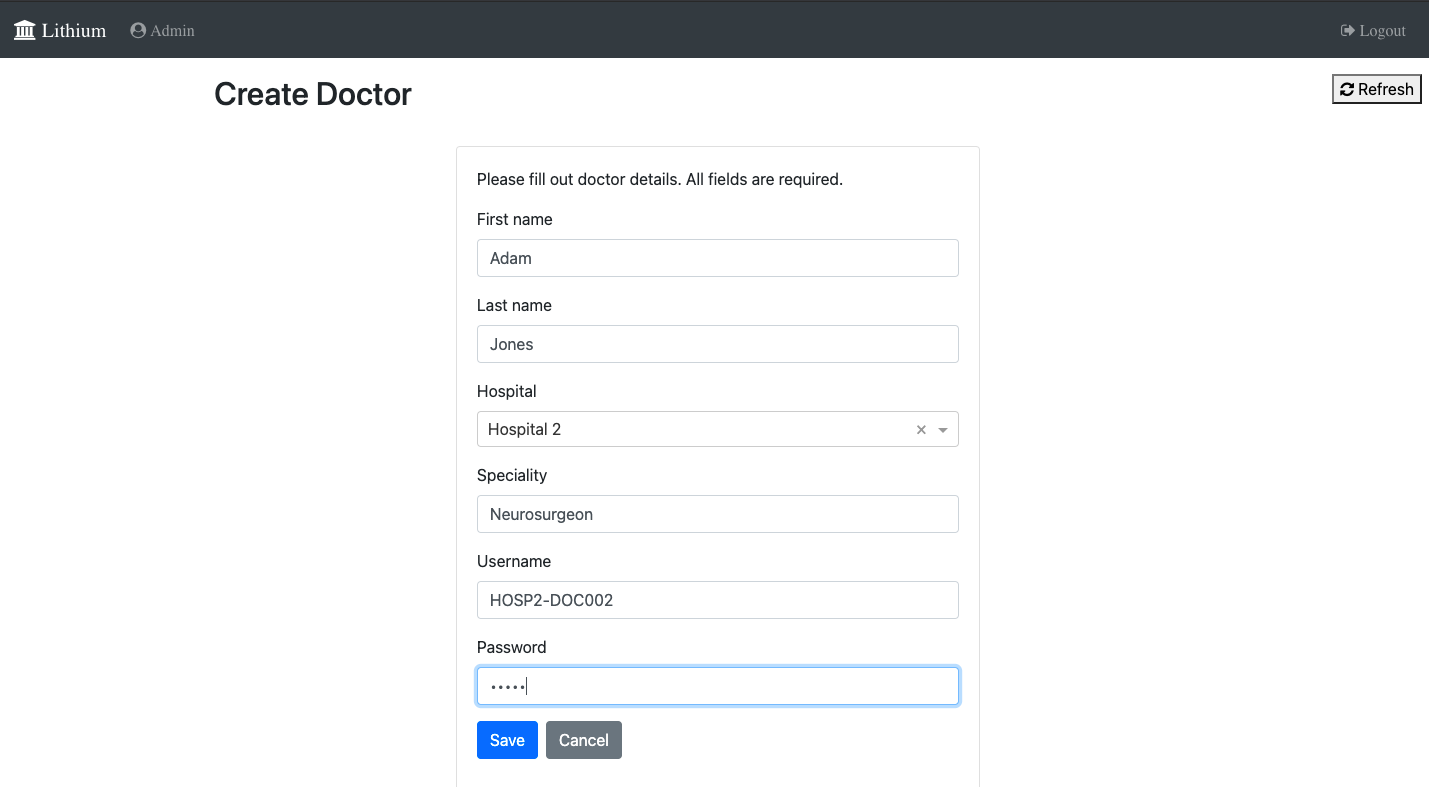
\includegraphics[height=8cm]{gfx/figures/admin6.png}
 \caption{Create Doctor}
 \label{fig:chapter03:admin6}
\end{figure}

\subsection{Login Patient}
The hospital provides patient his/her username and temporary password during the first visit to the hospital. If the patient is logging in for the first time, then after selecting role as patient and entering username and password provided by hospital, gets the message requesting to change the temporary password immediately as shown in Figure \ref{fig:chapter04:patient1}. The patient has to enter new password as per his/her choice as shown in Figure \ref{fig:chapter04:patient2}. The new password is then hashed and stored in ledger. So, from next time, whenever the patient wants to login, just has to select role, and enter username and new password. Both the temporary and new password are hashed and stored in the ledger. During every login, the entered password is hashed and compared with the hash value of password stored in ledger.
\begin{figure}[htbp]
 \centering
 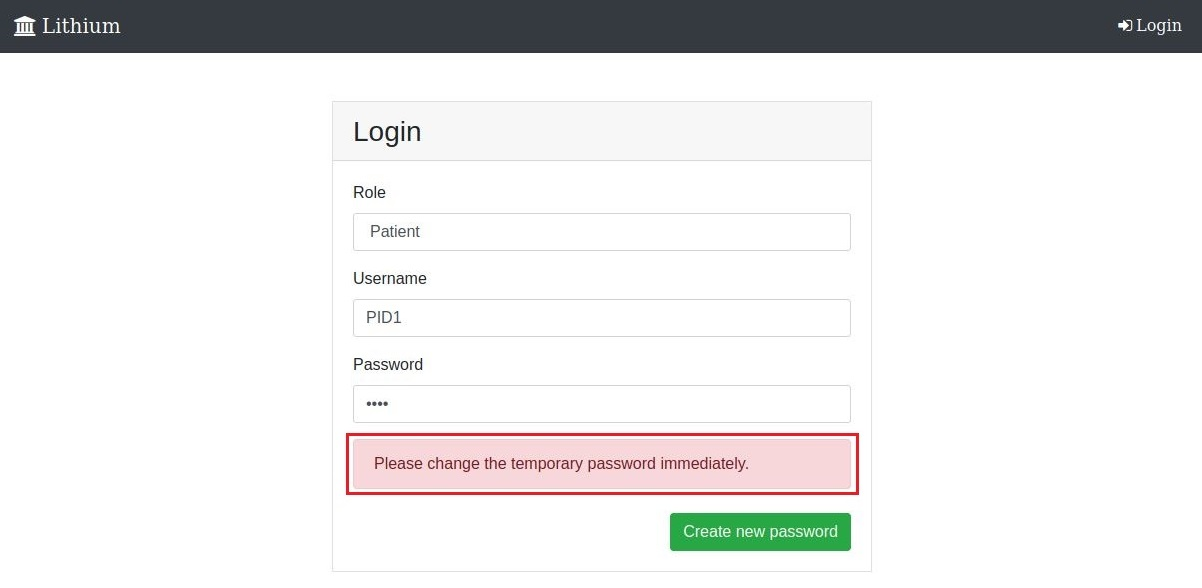
\includegraphics[width=1.1\textwidth, height=7.5cm]{gfx/figures/patient1.jpg}
 \caption{Login Patient}
 \label{fig:chapter04:patient1}
\end{figure}

\begin{figure}[htbp]
 \centering
 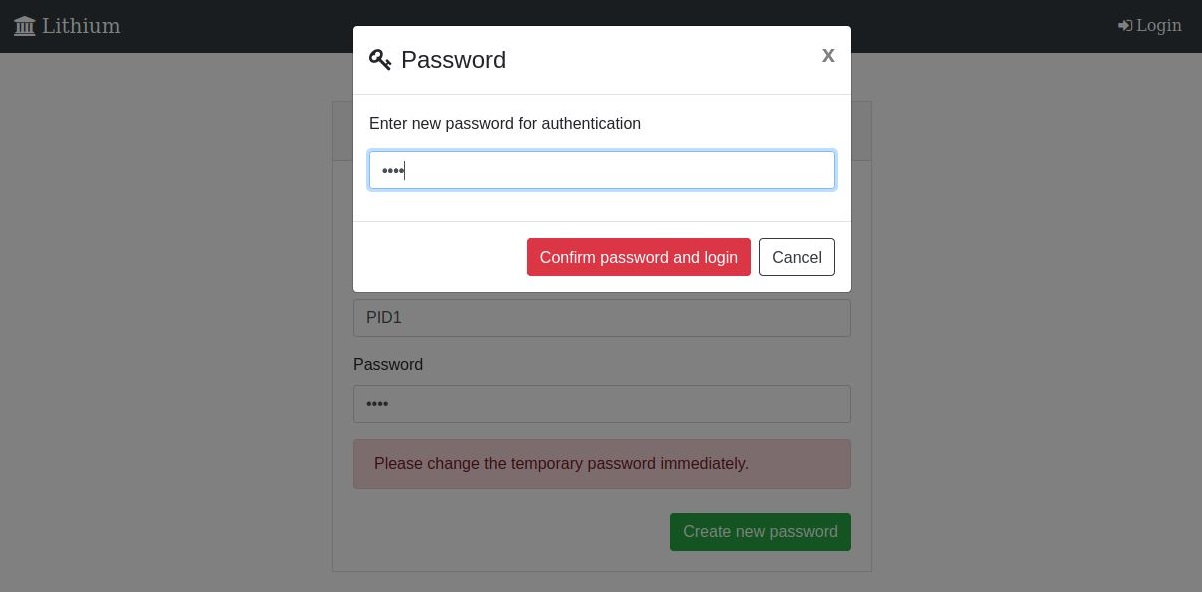
\includegraphics[width=1.1\textwidth, height=7.5cm]{gfx/figures/patient2.jpg}
 \caption{New Password}
 \label{fig:chapter04:patient2}
\end{figure}

\subsection{View Patient Details}
After successful login, the patient can view his/her personal as well as medical details as shown in Figure \ref{fig:chapter04:patient3}. The patient details are retrieved from the world state by invoking the patient contract.

\begin{figure}[htbp]
 \centering
 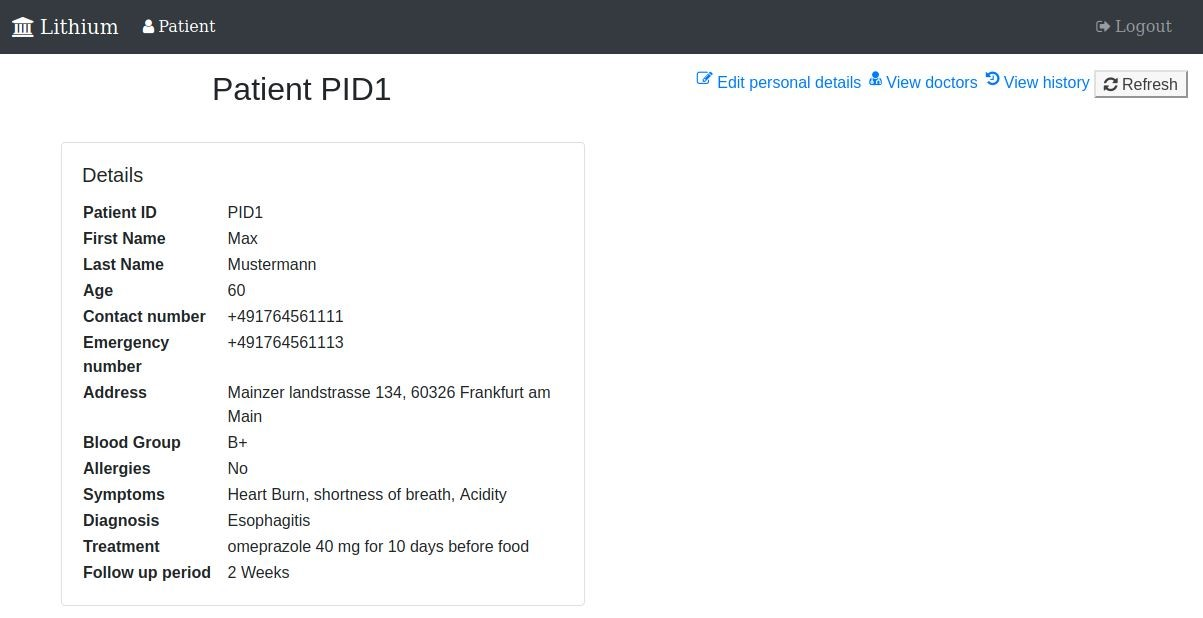
\includegraphics[width=1.1\textwidth, height=7cm]{gfx/figures/patient3.jpg}
 \caption{View Patient Details}
 \label{fig:chapter04:patient3}
\end{figure}

\subsection{Grant/Revoke Access}
On selecting \textit{View doctors}, it displays a list of doctors from both the hospitals  as shown in Figure \ref{fig:chapter04:patient4}. The patient has the right to grant or revoke the access to/from the doctor. When patient grants access to the doctor only then the doctor can view patient's medical details and medical history, When patient revokes the access, then doctor is unable to access patient's medical records, 

\begin{figure}[htbp]
 \centering
 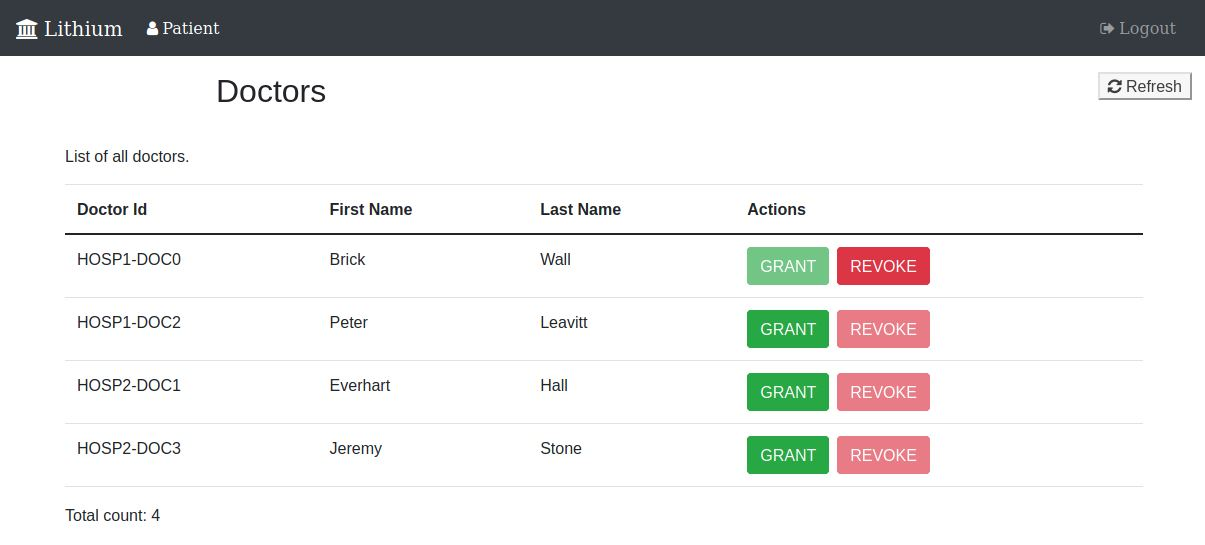
\includegraphics[width=1.1\textwidth, height=7cm]{gfx/figures/patient4.jpg}
 \caption{Grant/Revoke access}
 \label{fig:chapter04:patient4}
\end{figure}

\subsection{Edit Personal Details}
The patient can edit his/her personal details as shown in Figure \ref{fig:chapter04:patient5}. If any changes are made, then the new details are updated in the ledger using patient contract.

\begin{figure}[htbp]
 \centering
 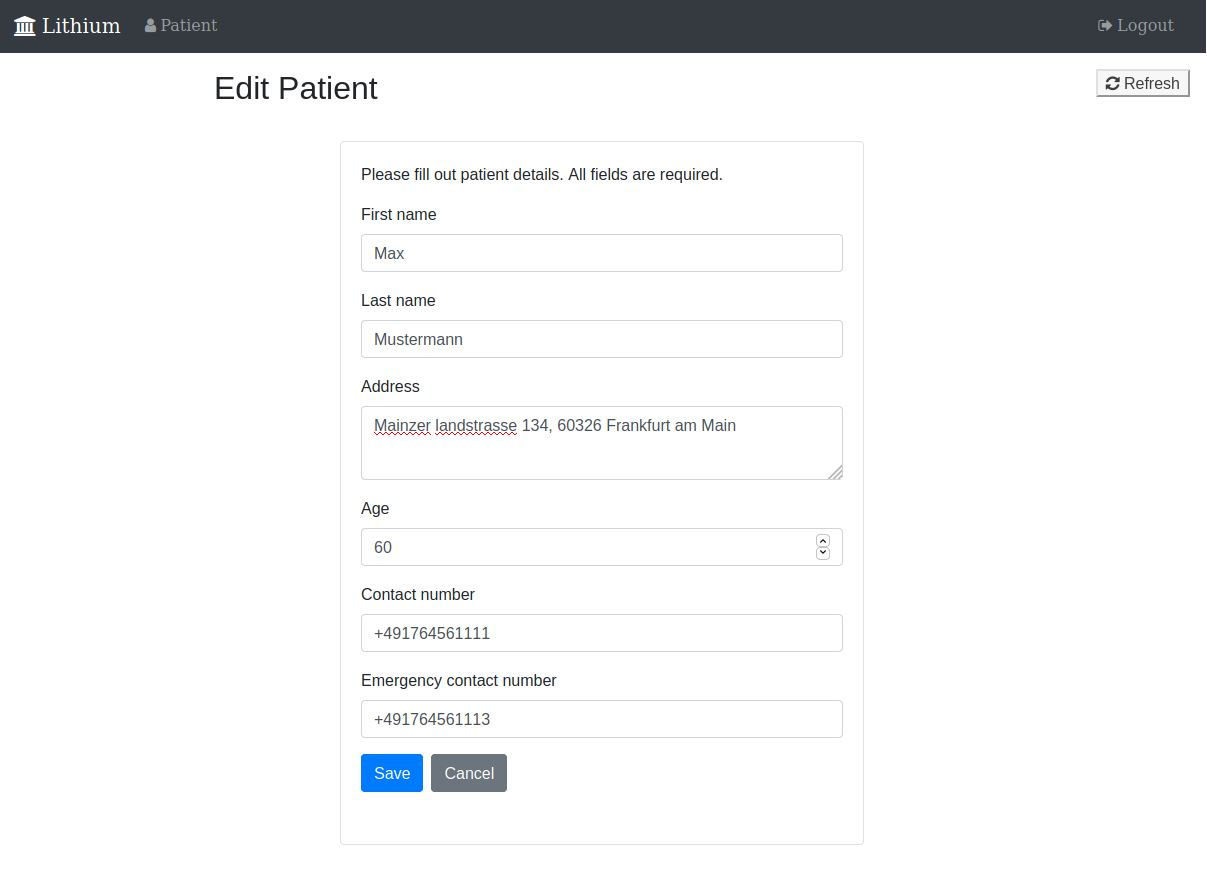
\includegraphics[width=1.1\textwidth, height=7cm]{gfx/figures/patient5.jpg}
 \caption{Edit personal details}
 \label{fig:chapter04:patient5}
\end{figure}

\subsection{View History}
The patient can view all the records, personal and medical starting from the first visit to the latest visit to all the doctors as shown in Figure \ref{fig:chapter04:patient5} . This functionality is possible because of the presence of getHistoryForKey API in hyperledger fabric which returns the history of the patient. This provides complete transparency of the transactions to the patient.

\begin{figure}[htbp]
 \centering
 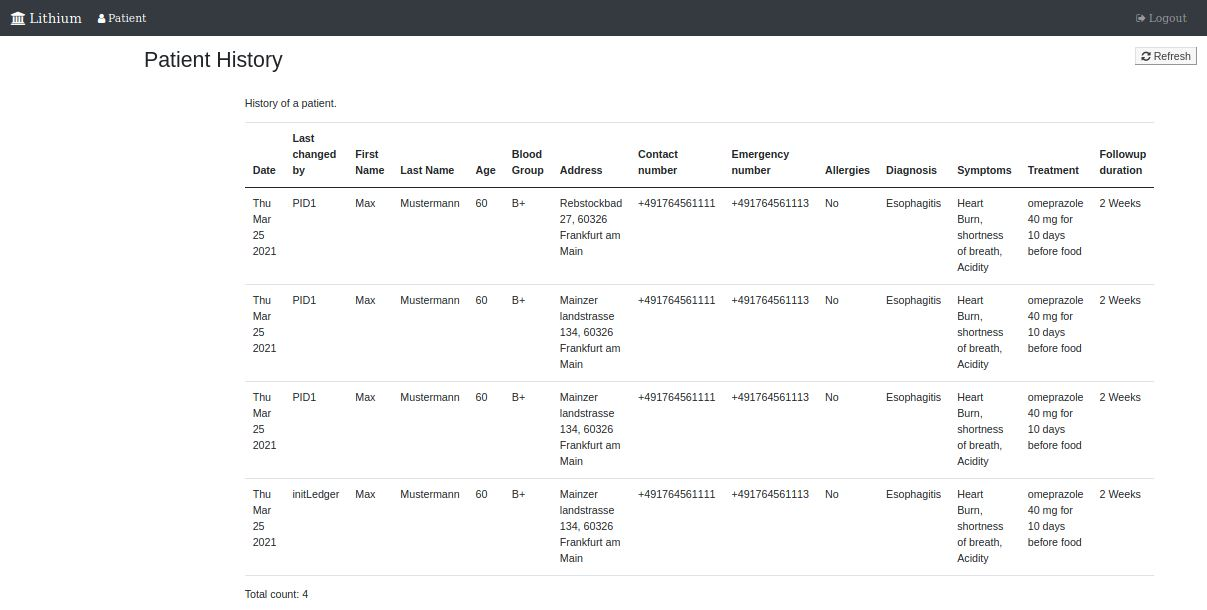
\includegraphics[width=1.1\textwidth, height=7cm]{gfx/figures/patient6.jpg}
 \caption{View patient's history}
 \label{fig:chapter04:patient6}
\end{figure}

\subsection{Login Doctor and View Doctor Details}
To login as doctor, user need to select 'Doctor' as a role, hospital which he/she belong and right credentials on login page as mentioned in the Figure \ref{fig:chapter04:doctor1}.

\begin{figure}[htbp]
 \centering
 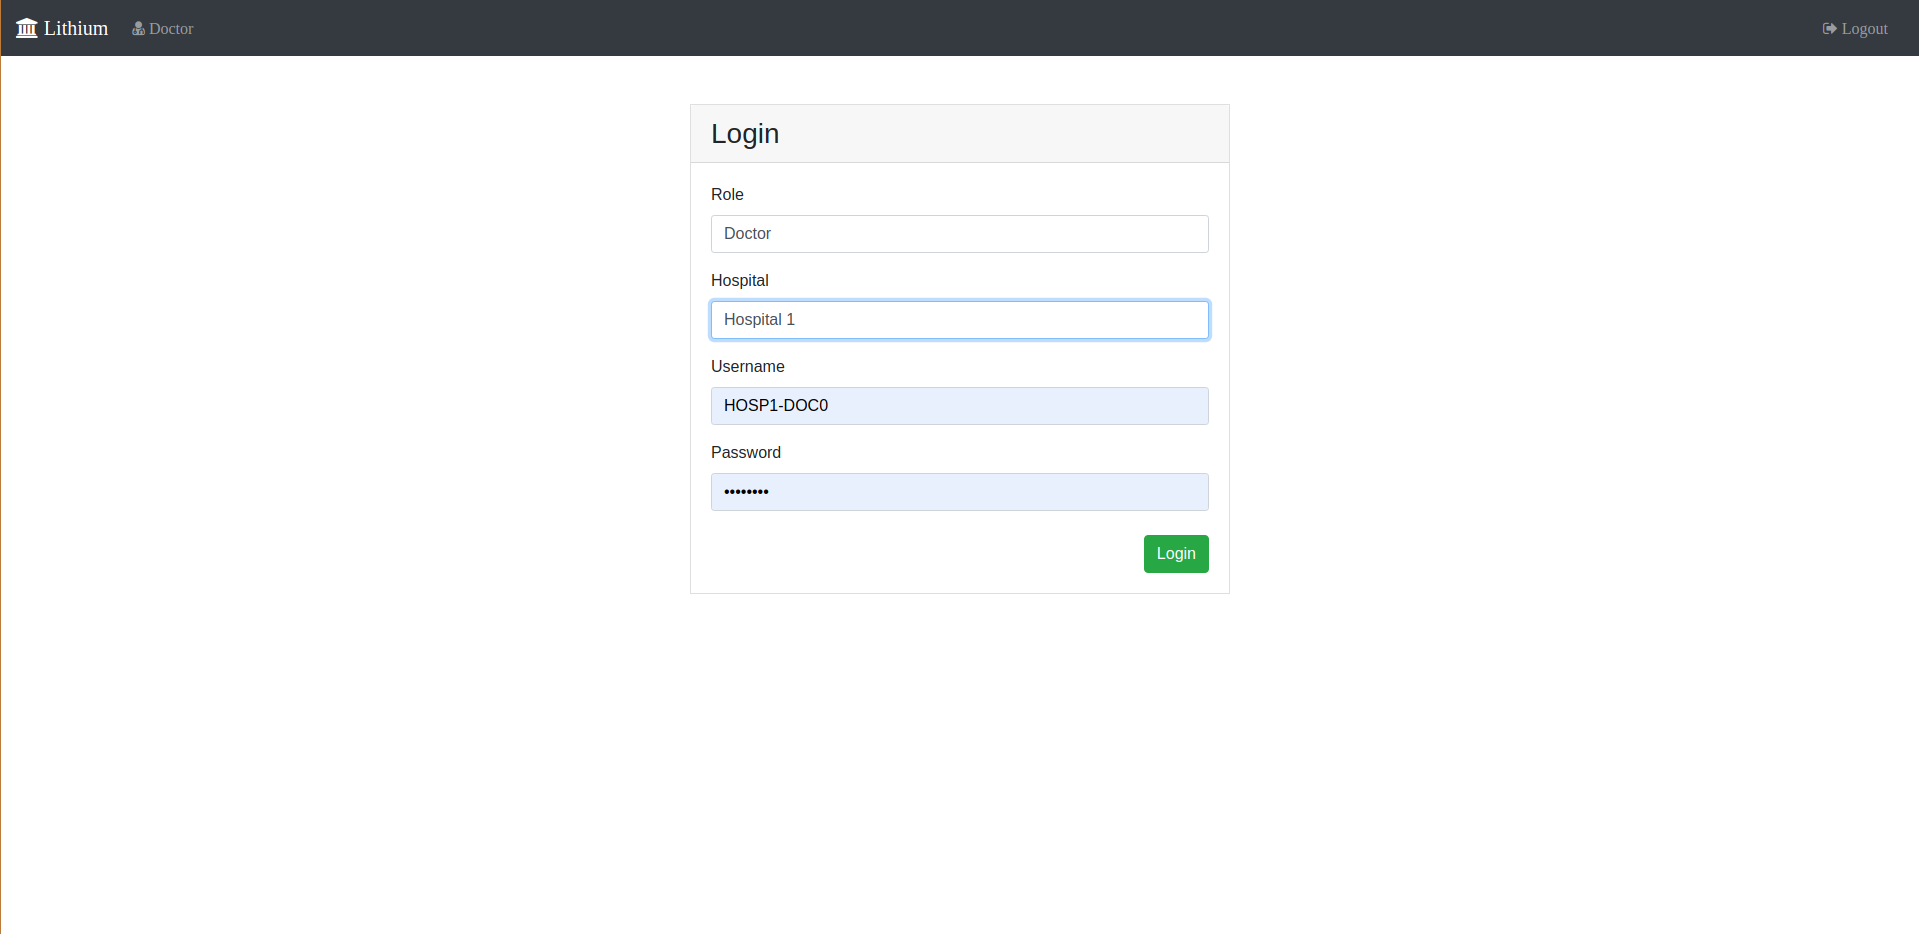
\includegraphics[width=1.1\textwidth, height=7cm]{gfx/figures/doctor1.png}
 \caption{Login Doctor}
 \label{fig:chapter04:doctor1}
\end{figure}

After successfully logged in as a doctor, the doctor details showed just like patient details. Here only few fields of the doctor shown in Figure \ref{fig:chapter04:doctor2}

\begin{figure}[htbp]
 \centering
 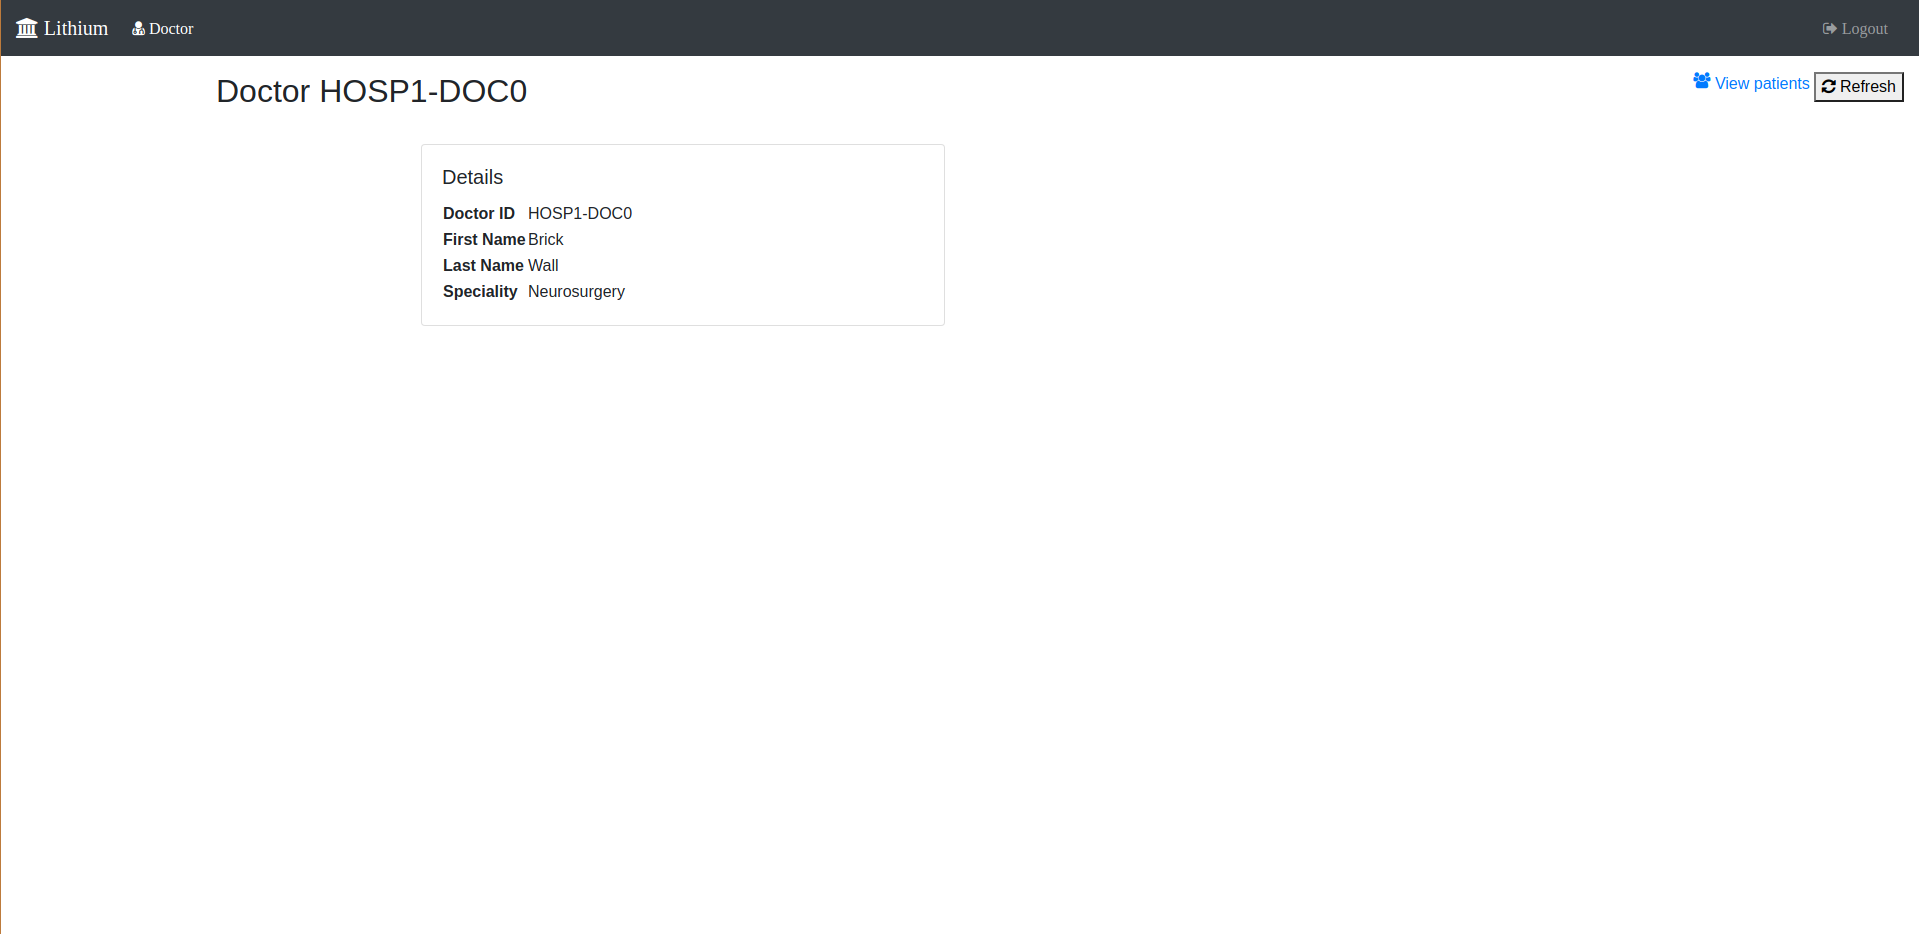
\includegraphics[width=1.1\textwidth, height=7cm]{gfx/figures/doctor2.png}
 \caption{View Doctor Details}
 \label{fig:chapter04:doctor2}
\end{figure}

\subsection{View Patients}
Doctor can view list of patients who provides access to him/her, otherwise list will be empty. In this case, the logged user doctor is 'HOSP1-DOC0' and patient PID1 provided access to this doctor. So in the list PID1 patient is visible in Figure \ref{fig:chapter04:doctor3}.

\begin{figure}[htbp]
 \centering
 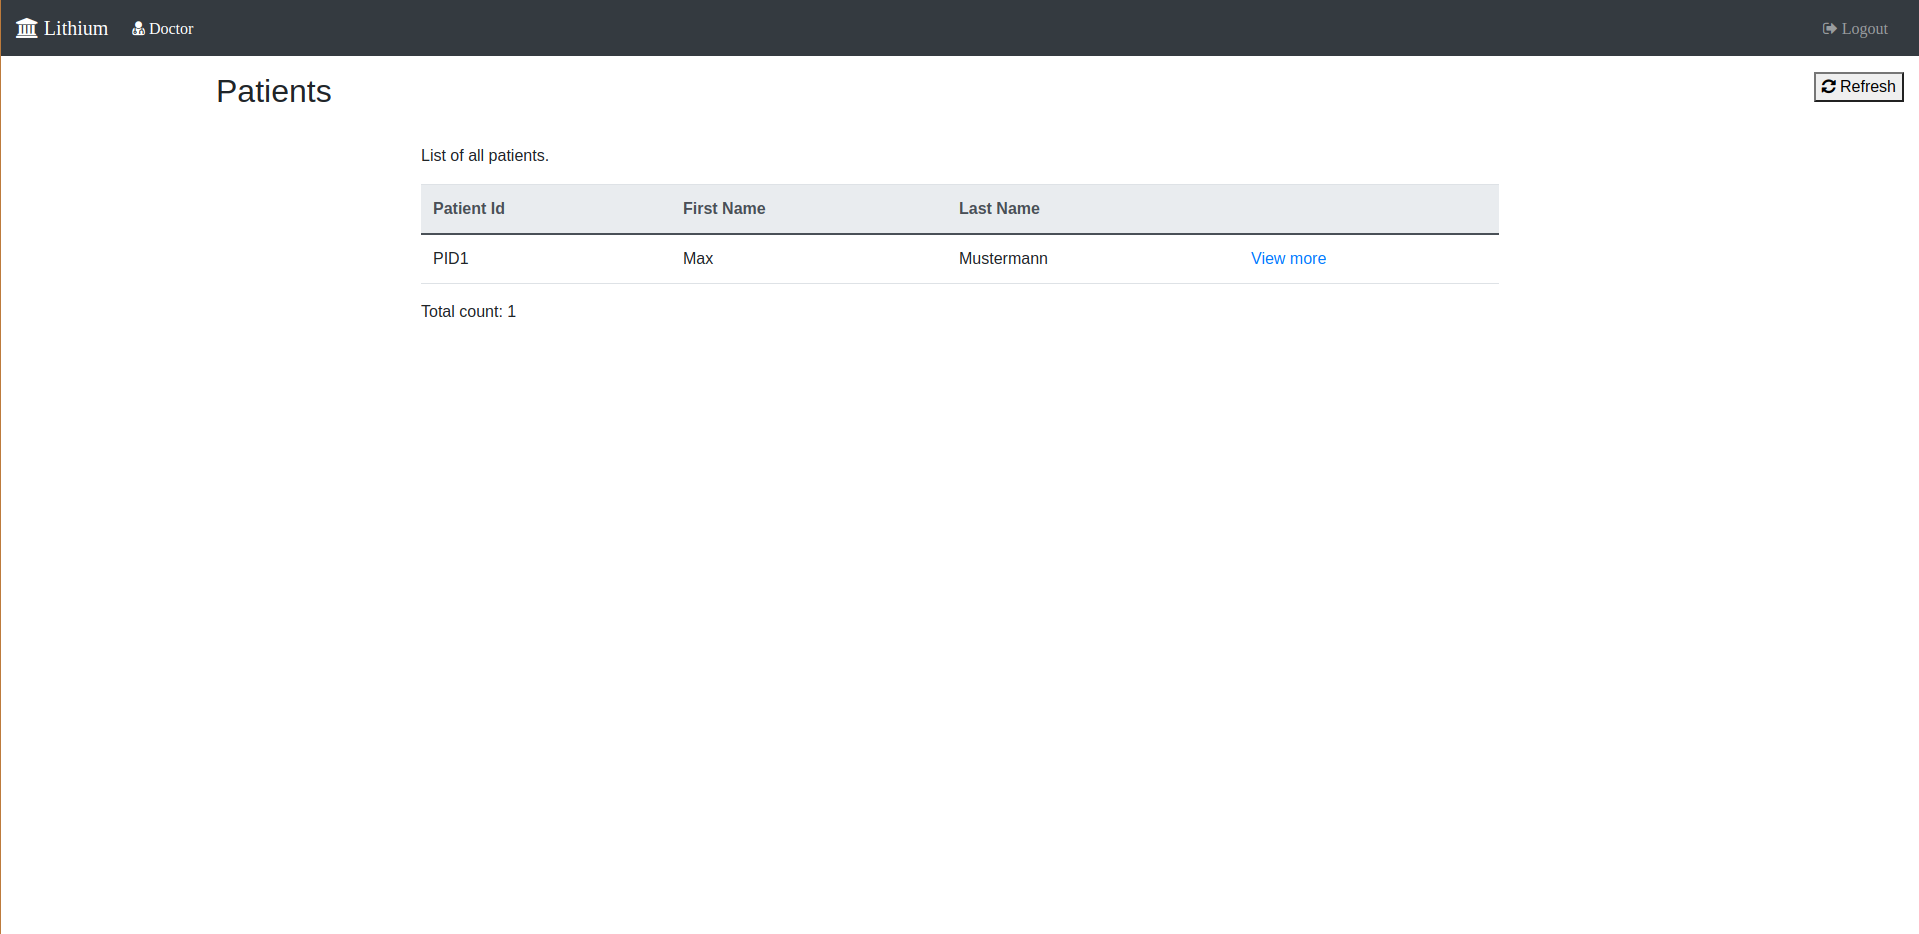
\includegraphics[width=1.1\textwidth, height=7cm]{gfx/figures/doctor3.png}
 \caption{List of patients}
 \label{fig:chapter04:doctor3}
\end{figure}

The list looks exactly same as to admin's dashboard, but doctor can see details of patient so in every entry there is a view more button as shown in Figure \ref{fig:chapter04:doctor3}. This redirects to patient details page, but only relevant fields are visible to doctor in Figure \ref{fig:chapter04:doctor4}. Here doctor can see the latest condition and information of the patient.

\begin{figure}[htbp]
 \centering
 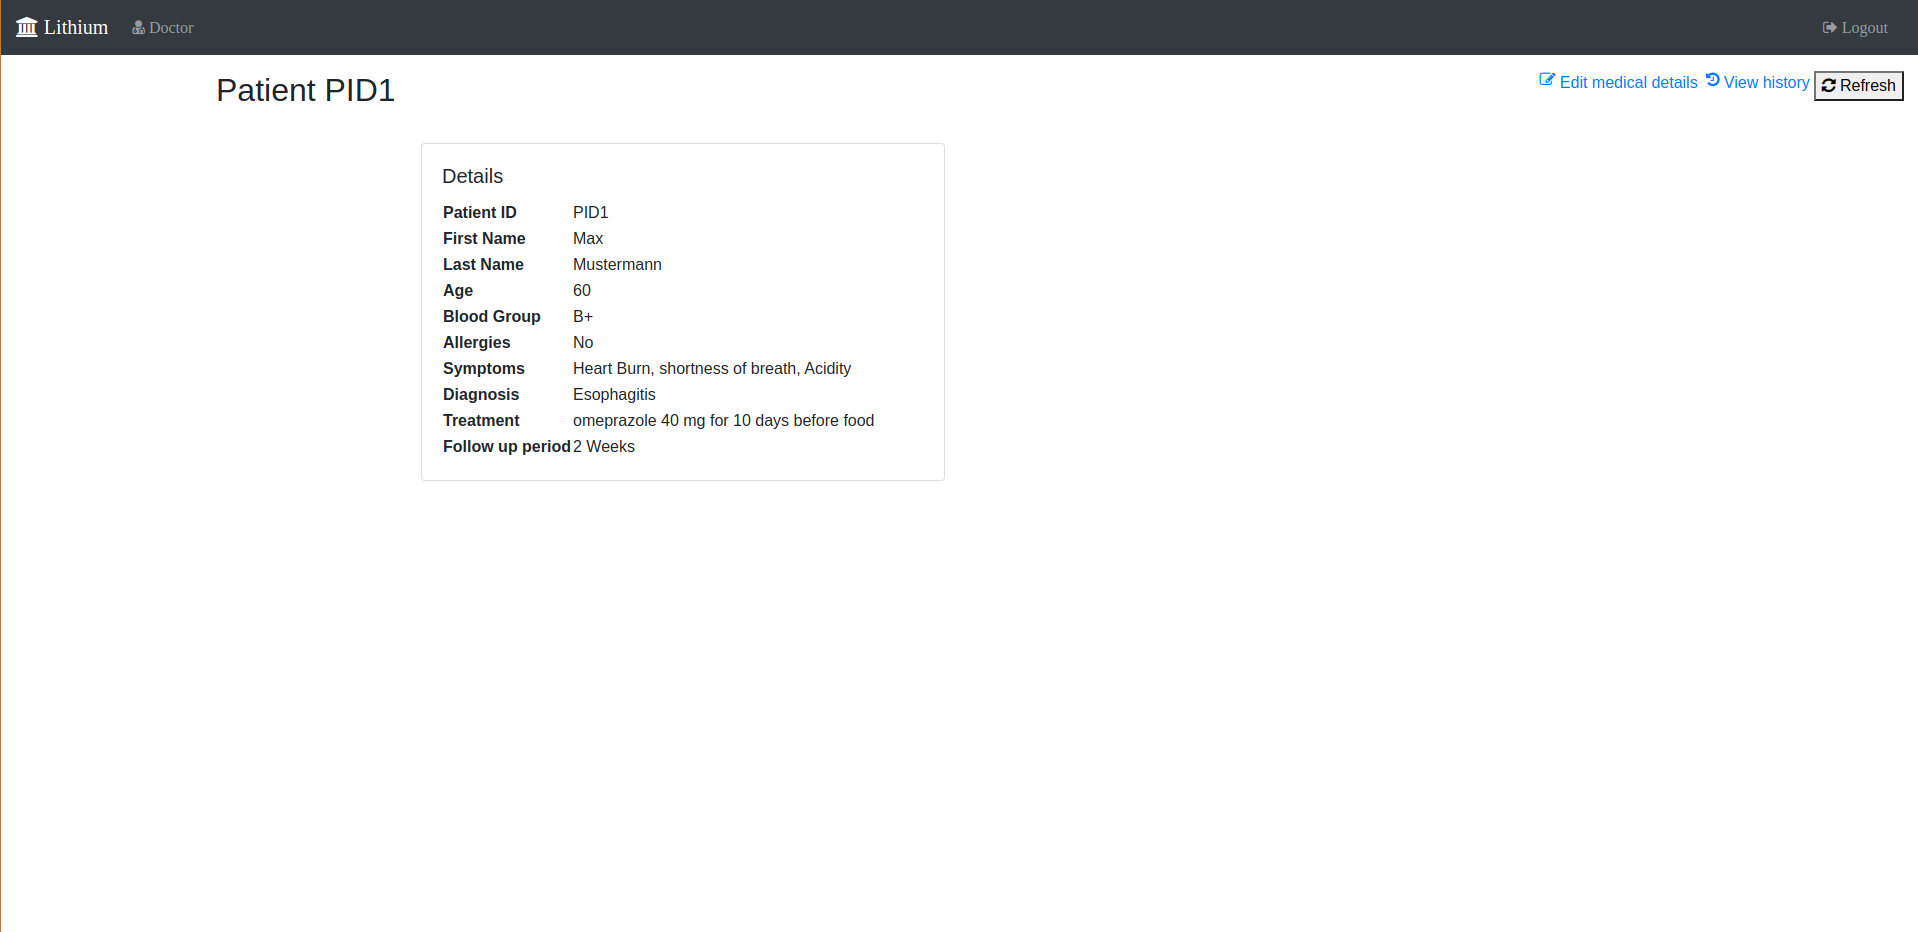
\includegraphics[width=1.1\textwidth, height=7cm]{gfx/figures/doctor4.png}
 \caption{View Patient Details}
 \label{fig:chapter04:doctor4}
\end{figure}

\subsection{Edit Medical Details}
Doctor can provide treatment by changing medical details of the patient in Figure \ref{fig:chapter04:doctor5}. On save button page redirected to patient details page.

\begin{figure}[htbp]
 \centering
 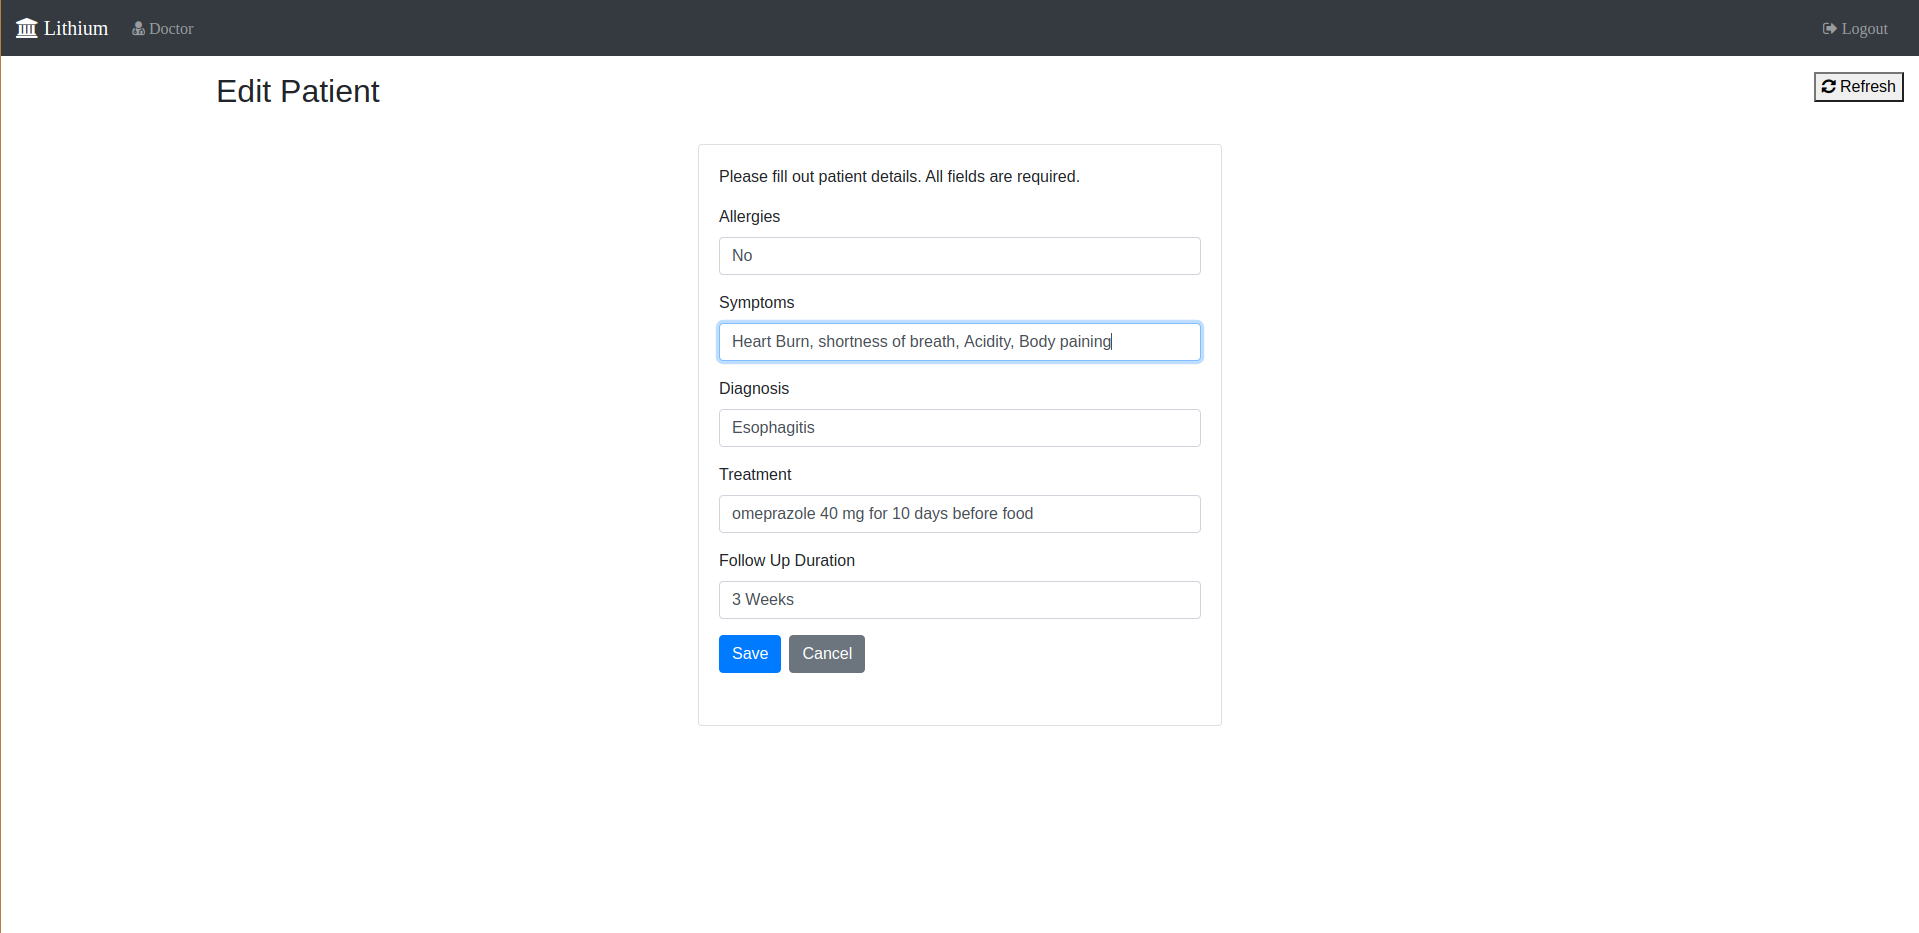
\includegraphics[width=1.1\textwidth, height=7cm]{gfx/figures/doctor5.png}
 \caption{Edit patient's medical details}
 \label{fig:chapter04:doctor5}
\end{figure}

\subsection{View History}
Doctor can view all history details of the patient which help doctor to understand patient's condition and can decide how the medication should be done. In Figure \ref{fig:chapter04:doctor6}. it shows same limited fields, as visible in patient details. In addition to those date and changed by info is also helpful to understand the treatment. 

\begin{figure}[htbp]
 \centering
 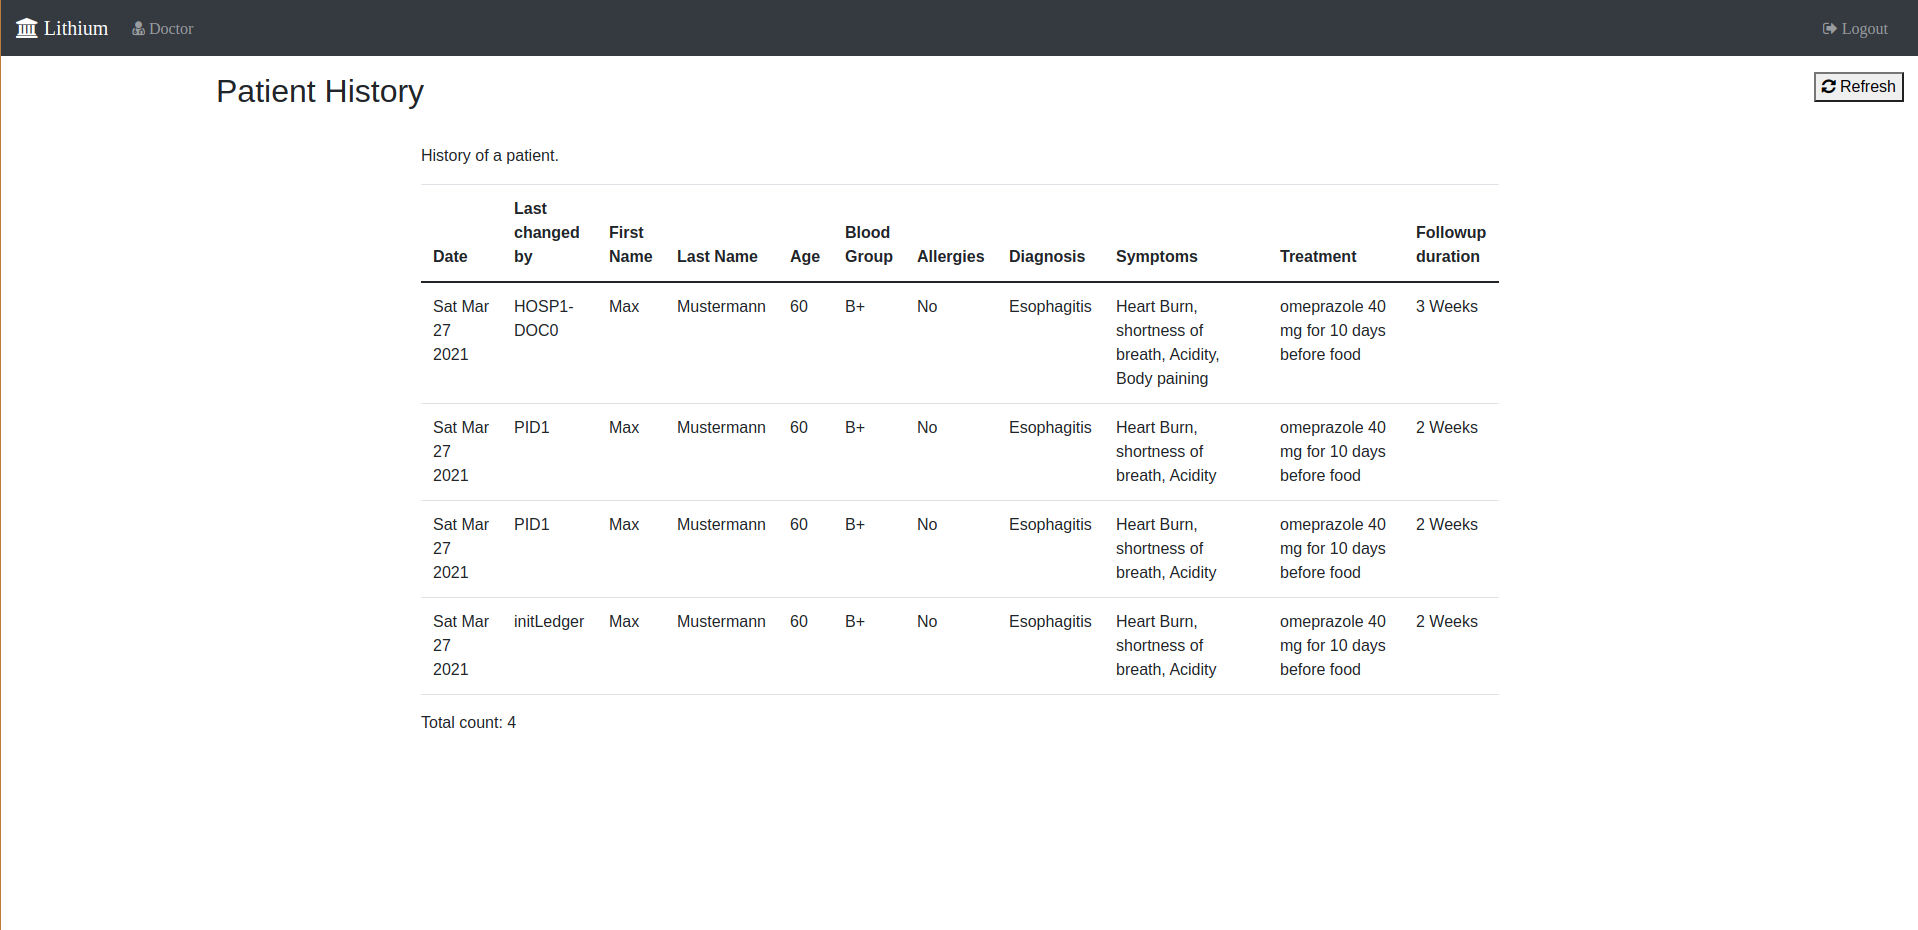
\includegraphics[width=1.1\textwidth, height=7cm]{gfx/figures/doctor6.png}
 \caption{View patient's history}
 \label{fig:chapter04:doctor6}
\end{figure}





\chapter{Results}
\label{ch:results}
%
% Section: Pros and Cons of using hyperledger
%
\section{Pros and Cons of using hyperledger Fabric}
This framework has some pros and cons.
\label{sec:results:proscons}
\subsection{Pros}
Fabric architecture allows the option to add plugins for the identity management and consensus algorithm. This helps companies having their own identity management system to integrate with fabric.
The main aim of companies using permissioned blockchain is the confidentiality of data. MSP component in fabric issues and validates certificates and provides user authentication. Data is secure since all the participants in the blockchain network are known. 
The \ac{PoW} algorithm is not used and hence mining is not required. This significantly optimizes the performance of the fabric. Fabric allows the creation of a private channel for only a few participants among a large blockchain network. There might be few transactions that should be viewed only by limited participants.

\subsection{Cons}
The architecture of hyperledger fabric is quite complex. It is not a fault-tolerant network. As of today fabric supports LevelDB and CouchDb. In the health care scenario, MRI reports and high resolution images need to stored, in such cases fabric provides limited database support.

%
% Section: Issues in hyperledger
%
\section{Issues in hyperledger}

% TODO: use admin credentials instead of doctor

\label{sec:results:issues}
Hyperledger Fabric project is an open-source blockchain platform that is still under development. New features and fixes are being developed every day. The following are some of the issues that were faced during the development of the application.


\subsection{getHistoryForKey - Private Data Collecion}
\label{sec:results:issues:getHistoryForKey}
% TODO: UPDATE THE LINK IN THE REFERENCES
In the current version of Hyperledger Fabric, the fabric doesn't support the API getHistoryForKey for a private data collection \cite{jira-5094}, however, this is a work in progress by the Hyperleder Fabric community which adds a history index and chaincode API similar to public data history to enable the query of history of a private data key. 

\subsection{Create a user defined role instead of client}

The current version of hyperledger fabric the only possible roles for \lstinline{hf.Registrar.Roles}  are Peer, client, and admin. The flaw with only 3 roles is, now all the clients have the same set of permission, but in a blockchain, there can be any number of types of roles and a set of permissions for each user-defined role. In the scenario, doctor and patient can be the user-defined roles rather than just the client. Doctor and patients can have their own set of rules to accomplish the issue mentioned in \ref{sec:results:issues:Access}. The fabric community is currently in progress to implement a way to add new hf.Registrar.(Delegate)Roles \cite{jira-548}.

\subsection{Access user attributes using client}
\label{sec:results:issues:Access}
In this scenario, as the doctor is not an asset to the ledger, the name and specialty of the doctor are stored in the attributes of the identity. However, the patients in the blockchain network cannot retrieve the attributes, as the patient does not have the access to read the doctor's attributes, but can be read using the admin user. This issue is due to the reason that a separate set of permissions cannot be applied as all the clients are considered to be the same. 
%
% Section: Challenges in the application
%
\section{Challenges in developing application}
\label{sec:results:challenges}
Major challenges are faced in implementing security on patient data in the ledger on a peer level. As there are two mechanisms described in \ref{sec:thesolution:securitymechanisms}. The private data collection approach is unable to apply due to fabric issues described in the above section. For data re-encryption, the approach fails to implement due to two major reasons. The first problem is, nodejs is lacking a decent library for re-encryption. Few libraries are available here \cite{nodejs-reencryption-libraries}. But none of them worked here. One has a working approach but does not fit regular system generated private and public keys. The format is not understandable by that library. Node-RSA is a very library for public-key cryptography and also accepts keys with the regular format, but does not have re-encryption functionality. There is an opportunity here to understand implement a re-encryption algorithm which is a time consuming task but a nice step as a separate small project and contributing to the community. The other problem is when a user gets created certificate and private key are generated. But not able to find a public key in the fabric framework. More research is required to diagnose this issue and make re-encryption mechanism work.
Next challenge faced in scaling peers of hospital organizations. For some reason, one fabric-peer container always stops when the network gets up. In addition to that when generating ccp files, not all peer configurations are included. The work is in progress and \href{https://github.com/kshitijyelpale/blockchain-hyperledger-fabric-electronic-patient-records/pull/51}{draft pull request is opened}.



\chapter{Conclusion and Future Work}
\label{ch:conclusion}

%
% Section: conclusion
%
\section{Conclusion}
\label{sec:conclusion:Conclusion}

Hyperledger fabric is a promising blockchain framework that has some concepts of policies, smart contracts, and provision of secure identities which make the records secure and controlled. It enables the EHR systems to interoperable among multiple hospital organizations. Doctors can track history easily. Patients do not need to carry medical history files and will be significant improvements in digital records. 

An EHR scenario comes under the private and closed blockchain category and this solution can successfully conclude that it is an encouraging framework of this kind of blockchain. It provides a reliable and secure solution in managing medical field record

%
% Section: Future Work
%
\section{Future Work}
\label{sec:conclusion:futurework}

Many improvements can be done to improve the solution, make a production-grade application. Even though blockchain and fabric provide tons of security by default in their framework and concept, still need to overcome the security challenges discussed above and implement successful security for the patient records. Though the fabric framework is quite pluggable by itself, the source code can be improved to make the solution more pluggable when adding more hospitals and its peers. As the network scales up, more organizations and peers are connected to the channel, and to handle many transaction requests and approvals, many ordering peers are needed to speed up the process. Apaches Kafka, an open-source distributed event streaming platform is a very promising tool to manage multiple ordering nodes. 

Design consortium policy in such a way that minimum criteria of consensus algorithm can be satisfied. The fabric uses pBFT in which all peers' approval is needed to approve transactions, such as 75\%approving criteria it means 3 out of 4 peer's approval is sufficient to make a transaction. Distribute the wallet as per the organization's peers. The users created at the wallet should be stored to their respective organization peers. The wallet can also be stored in the no-SQL database and replicate to multiple nodes to avoid data loss. 

The network calls in the network should be done via HTTPS which provides transport-level security (TLS). Currently, from the front end to the back end, passwords are sent in plain text which can be improved by this. For temporary password integration of email, functionality is the best approach. Moreover adaption of forgetting password functionality is good to have. UI/UX strategies can be applied to make enhance the experience. Search functionality can be useful when patients' data go beyond the limit. But need to research that if fabric supports wildcard searches or not. Again the data is not coming from a single database so it is important that frequent search queries can not be possible.

The application should have the test cases to run the application in a production environment. Few test cases are available but it should have a test case for unit, integration, public REST API, and end-to-end cases. The existing test case was written using the Cypress framework which is an E2E testing framework. An application can be deployed using Kubernetes for the production environment. As the network grows the more hospitals with their peers and channels exist in the network. So Kubernetes is the best orchestration tool to manage all these containers.

%\include{chapters/chapter_zzz_example}

%*************************************************************************
% Backmatter
%*************************************************************************
\appendix
\renewcommand{\thechapter}{\alph{chapter}}
\cleardoublepage
%\part{Appendix}
%%************************************************
%\chapter{Introduction to the Classic Thesis style}
%\label{ch:classicthesis}
%************************************************
% The ClassicThesis bundle for \LaTeX\ has two goals:
% \begin{enumerate}
%     \item Provide students with an easy-to-use template for their
%     Master's
%     or PhD thesis. (Though it might also be used by other types of
%     authors
%     for reports, books, etc.)
%     \item Provide a classic, high-quality typographic style that is
%     inspired by \citeauthor{bringhurst:2002}'s ``\emph{The Elements of
%     Typographic Style}'' \citep{bringhurst:2002}.
%     \marginpar{\myTitle \myVersion}
% \end{enumerate}
% The bundle is configured to run with a \emph{full}
% MiK\TeX\ or \TeX Live\footnote{See the file \texttt{LISTOFFILES} for
% needed packages. Furthermore, \texttt{classicthesis}
% works with most other distributions and, thus, with most systems
% \LaTeX\ is available for.}
% installation right away and, therefore, it uses only freely available
% fonts. (Minion fans can easily adjust the style to their needs.)

% People interested only in the nice style and not the whole bundle can
% now use the style stand-alone via the file \texttt{classicthesis.sty}.
% This works now also with ``plain'' \LaTeX.

% As of version 3.0, \texttt{classicthesis} can also be easily used with
% \mLyX\footnote{\url{http://www.lyx.org}} thanks to Nicholas Mariette
% and Ivo Pletikosić. The \mLyX\ version of this manual will contain
% more information on the details.

% This should enable anyone with a basic knowledge of \LaTeXe\ or \mLyX\ to
% produce beautiful documents without too much effort. In the end, this
% is my overall goal: more beautiful documents, especially theses, as I
% am tired of seeing so many ugly ones.

% The whole template and the used style is released under the
% \acsfont{GNU} General Public License.

% If you like the style then I would appreciate a postcard:
% \begin{center}
%     André Miede \\
%     Detmolder Straße 32 \\
%     31737 Rinteln \\
%     Germany
% \end{center}
% The postcards I received so far are available at:
% \begin{center}
%     \url{http://postcards.miede.de}
% \end{center}
% \marginpar{A well-balanced line width improves the legibility of
% the text. That's what typography is all about, right?}
% So far, many theses, some books, and several other publications have
% been typeset successfully with it. If you are interested in some
% typographic details behind it, enjoy Robert Bringhurst's wonderful book.
% % \citep{bringhurst:2002}.

% \paragraph{Important Note:} Some things of this style might look
% unusual at first glance, many people feel so in the beginning.
% However, all things are intentionally designed to be as they are,
% especially these:
% \begin{itemize}
%     \item No bold fonts are used. Italics or spaced small caps do the
%     job quite well.
%     \item The size of the text body is intentionally shaped like it
%     is. It supports both legibility and allows a reasonable amount of
%     information to be on a page. And, no: the lines are not too short.
%     \item The tables intentionally do not use vertical or double
%     rules. See the documentation for the \texttt{booktabs} package for
%     a nice discussion of this topic.\footnote{To be found online at
%     \url{http://mirror.ctan.org/macros/latex/contrib/booktabs/}.}
%     \item And last but not least, to provide the reader with a way
%     easier access to page numbers in the table of contents, the page
%     numbers are right behind the titles. Yes, they are \emph{not}
%     neatly aligned at the right side and they are \emph{not} connected
%     with dots that help the eye to bridge a distance that is not
%     necessary. If you are still not convinced: is your reader
%     interested in the page number or does she want to sum the numbers
%     up?
% \end{itemize}
% Therefore, please do not break the beauty of the style by changing
% these things unless you really know what you are doing! Please.

% \paragraph{Yet Another Important Note:} Since \texttt{classicthesis}'
% first release in 2006, many things have changed in the \LaTeX\ world.
% Trying to keep up-to-date, \texttt{classicthesis} grew and evolved
% into many directions, trying to stay (some kind of) stable and be
% compatible with its port to \mLyX. However, there are still many
% remains from older times in the code, many dirty workarounds here and
% there, and several other things I am absolutely not proud of (for
% example my unwise combination of \acsfont{KOMA} and
% \texttt{titlesec} etc.).
% \graffito{An outlook into the future of \texttt{classicthesis}.}

% Currently, I am looking into how to completely re-design and
% re-implement \texttt{classicthesis} making it easier to maintain and
% to use. As a general idea, \texttt{classicthesis.sty} should be
% developed and distributed separately from the template bundle itself.
% Excellent spin-offs such as \texttt{arsclassica} could also be
% integrated (with permission by their authors) as format configurations.
% Also, current trends of \texttt{microtype}, \texttt{fontspec}, etc.
% should be included as well. As I am not really into deep
% \LaTeX\ programming,
% I will reach out to the \LaTeX\ community for their expertise and help.


% \section{Organization}
% A very important factor for successful thesis writing is the
% organization of the material. This template suggests a structure as
% the following:
% \begin{itemize}
%     \marginpar{You can use these margins for summaries of the text
%     body\dots}
%     \item\texttt{Chapters/} is where all the ``real'' content goes in
%     separate files such as \texttt{Chapter01.tex} etc.
%     % \item\texttt{Examples/} is where you store all listings and other
%     % examples you want to use for your text.
%     \item\texttt{FrontBackMatter/} is where all the stuff goes that
%     surrounds the ``real'' content, such as the acknowledgments,
%     dedication, etc.
%     \item\texttt{gfx/} is where you put all the graphics you use in
%     the thesis. Maybe they should be organized into subfolders
%     depending on the chapter they are used in, if you have a lot of
%     graphics.
%     \item\texttt{Bibliography.bib}: the Bib\TeX\ database to organize
%     all the references you might want to cite.
%     \item\texttt{classicthesis.sty}: the style definition to get this
%     awesome look and feel. Does not only work with this thesis template
%     but also on its own (see folder \texttt{Examples}). Bonus: works
%     with both \LaTeX\ and \textsc{pdf}\LaTeX\dots and \mLyX.
%     % \item\texttt{ClassicThesis.tcp} a \TeX nicCenter project file.
%     Great tool and it's free!
%     \item\texttt{ClassicThesis.tex}: the main file of your thesis
%     where all gets bundled together.
%     \item\texttt{classicthesis-config.tex}: a central place to load all
%     nifty packages that are used. % In there, you can also activate
%     % backrefs in order to have information in the bibliography about
%     % where a source was cited in the text (\ie, the page number).

%     \emph{Make your changes and adjustments here.} This means that you
%     specify here the options you want to load \texttt{classicthesis.sty}
%     with. You also adjust the title of your thesis, your name, and all
%     similar information here. Refer to \autoref{sec:custom} for more
%     information.

%     This had to change as of version 3.0 in order to enable an easy
%     transition from the ``basic'' style to \mLyX.
% \end{itemize}
% In total, this should get you started in no time.


% \clearpage
% \section{Style Options}\label{sec:options}
% There are a couple of options for \texttt{classicthesis.sty} that
% allow for a bit of freedom concerning the layout:
% \marginpar{\dots or your supervisor might use the margins for some
%     comments of her own while reading.}
% \begin{itemize}
%     \item General:
%         \begin{itemize}
%             \item\texttt{drafting}: prints the date and time at the bottom of
%             each page, so you always know which version you are dealing with.
%             Might come in handy not to give your Prof. that old draft.
%         \end{itemize}

%     \item Parts and Chapters:
%         \begin{itemize}
%             \item\texttt{parts}: if you use Part divisions for your document,
%             you should choose this option. (Cannot be used together with
%             \texttt{nochapters}.)

%             \item\texttt{linedheaders}: changes the look of the chapter
%             headings a bit by adding a horizontal line above the chapter
%             title. The chapter number will also be moved to the top of the
%             page, above the chapter title.
%         \end{itemize}

%     \item Typography:
%         \begin{itemize}
%             \item\texttt{eulerchapternumbers}: use figures from Hermann Zapf's
%             Euler math font for the chapter numbers. By default, old style
%             figures from the Palatino font are used.

%             \item\texttt{beramono}: loads Bera Mono as typewriter font.
%             (Default setting is using the standard CM typewriter font.)

%             \item\texttt{eulermath}: loads the awesome Euler fonts for math.
%             Pala\-tino is used as default font.
%         \end{itemize}

%     \marginpar{Options are enabled via \texttt{option=true}}

%     \item Table of Contents:
%         \begin{itemize}
%             \item\texttt{tocaligned}: aligns the whole table of contents on
%             the left side. Some people like that, some don't.

%             \item\texttt{dottedtoc}: sets pagenumbers flushed right in the
%             table of contents.

%             \item\texttt{manychapters}: if you need more than nine chapters for
%             your document, you might not be happy with the spacing between the
%             chapter number and the chapter title in the Table of Contents.
%             This option allows for additional space in this context.
%             However, it does not look as ``perfect'' if you use
%             \verb|\parts| for structuring your document.
%         \end{itemize}

%     \item Floats:
%         \begin{itemize}
%             \item\texttt{listings}: loads the \texttt{listings} package (if not
%             already done) and configures the List of Listings accordingly.

%             \item\texttt{floatperchapter}: activates numbering per chapter for
%             all floats such as figures, tables, and listings (if used).
%         \end{itemize}

% \end{itemize}

% Furthermore, pre-defined margins for different paper sizes are available, \eg, \texttt{a4paper}, \texttt{a5paper}, and \texttt{letterpaper}. These are based on your chosen option of \verb|\documentclass|.

% The best way to figure these options out is to try the different
% possibilities and see what you and your supervisor like best.

% In order to make things easier, \texttt{classicthesis-config.tex}
% contains some useful commands that might help you.


% \section{Customization}\label{sec:custom}
% %(As of v3.0, the Classic Thesis Style for \LaTeX{} and \mLyX{} share
% %the same two \texttt{.sty} files.)
% This section will show you some hints how to adapt
% \texttt{classicthesis} to your needs.

% The file \texttt{classicthesis.sty}
% contains the core functionality of the style and in most cases will
% be left intact, whereas the file \texttt{classic\-thesis-config.tex}
% is used for some common user customizations.

% The first customization you are about to make is to alter the document
% title, author name, and other thesis details. In order to do this, replace
% the data in the following lines of \texttt{classicthesis-config.tex:}%
% \marginpar{Modifications in \texttt{classic\-thesis-config.tex}%
% }

% \begin{lstlisting}
%     % **************************************************
%     % 2. Personal data and user ad-hoc commands
%     % **************************************************
%     \newcommand{\myTitle}{A Classic Thesis Style\xspace}
%     \newcommand{\mySubtitle}{An Homage to...\xspace}
% \end{lstlisting}

% Further customization can be made in \texttt{classicthesis-config.tex}
% by choosing the options to \texttt{classicthesis.sty}
% (see~\autoref{sec:options}) in a line that looks like this:

% \begin{lstlisting}
%   \PassOptionsToPackage{
%     drafting=true,    % print version information on the bottom of the pages
%     tocaligned=false, % the left column of the toc will be aligned (no indentation)
%     dottedtoc=false,  % page numbers in ToC flushed right
%     parts=true,       % use part division
%     eulerchapternumbers=true, % use AMS Euler for chapter font (otherwise Palatino)
%     linedheaders=false,       % chaper headers will have line above and beneath
%     floatperchapter=true,     % numbering per chapter for all floats (i.e., Figure 1.1)
%     listings=true,    % load listings package and setup LoL
%     subfig=true,      % setup for preloaded subfig package
%     eulermath=false,  % use awesome Euler fonts for mathematical formulae (only with pdfLaTeX)
%     beramono=true,    % toggle a nice monospaced font (w/ bold)
%     minionpro=false   % setup for minion pro font; use minion pro small caps as well (only with pdfLaTeX)
%   }{classicthesis}
% \end{lstlisting}

% Many other customizations in \texttt{classicthesis-config.tex} are
% possible, but you should be careful making changes there, since some
% changes could cause errors.

% % Finally, changes can be made in the file \texttt{classicthesis.sty},%
% % \marginpar{Modifications in \texttt{classicthesis.sty}%
% % } although this is mostly not designed for user customization. The
% % main change that might be made here is the text-block size, for example,
% % to get longer lines of text.


% \section{Issues}\label{sec:issues}
% This section will list some information about problems using
% \texttt{classic\-thesis} in general or using it with other packages.

% Beta versions of \texttt{classicthesis} can be found at Bitbucket:
% \begin{center}
%     \url{https://bitbucket.org/amiede/classicthesis/}
% \end{center}
% There, you can also post serious bugs and problems you encounter.


% \section{Future Work}
% So far, this is a quite stable version that served a couple of people
% well during their thesis time. However, some things are still not as
% they should be. Proper documentation in the standard format is still
% missing. In the long run, the style should probably be published
% separately, with the template bundle being only an application of the
% style. Alas, there is no time for that at the moment\dots it could be
% a nice task for a small group of \LaTeX nicians.

% Please do not send me email with questions concerning \LaTeX\ or the
% template, as I do not have time for an answer. But if you have
% comments, suggestions, or improvements for the style or the template
% in general, do not hesitate to write them on that postcard of yours.


% \section{Beyond a Thesis}
% The layout of \texttt{classicthesis.sty} can be easily used without the
% framework of this template. A few examples where it was used to typeset
% an article, a book or a curriculum vitae can be found in the folder
% \texttt{Examples}. The examples have been tested with
% \texttt{latex} and \texttt{pdflatex} and are easy to compile. To
% encourage you even more, PDFs built from the sources can be found in the
% same folder.


% \section{License}
% \paragraph{GNU General Public License:} This program is free software;
% you can redistribute it and/or modify
% it under the terms of the \acsfont{GNU} General Public License as
% published by
% the Free Software Foundation; either version 2 of the License, or
% (at your option) any later version.

% This program is distributed in the hope that it will be useful,
% but \emph{without any warranty}; without even the implied warranty of
% \emph{merchant\-ability} or \emph{fitness for a particular purpose}.
% See the
% \acsfont{GNU} General Public License for more details.

% You should have received a copy of the \acsfont{GNU} General
% Public License
% along with this program; see the file \texttt{COPYING}.  If not,
% write to
% the Free Software Foundation, Inc., 59 Temple Place - Suite 330,
% Boston, MA 02111-1307, USA.

% \paragraph{classichthesis Authors' note:} There have been some discussions about the GPL's implications on using \texttt{classicthesis} for theses etc. Details can be found here:
% \begin{center}
%   \url{https://bitbucket.org/amiede/classicthesis/issues/123/}
% \end{center}

% We chose (and currently stick with) the GPL because we would not like to compete with proprietary modified versions of our own work. However, the whole template is free as free beer and free speech. We will not demand the sources for theses, books, CVs, etc. that were created using \texttt{classicthesis}.

% Postcards are still highly appreciated.





%*****************************************
%*****************************************
%*****************************************
%*****************************************
%*****************************************

\chapter{Authors}

Abstract - Varsha and Jathin
\begin{enumerate}
    \item Introduction
    \begin{enumerate} [label=1.\arabic*]
        \item Background - Varsha
        \item Existing Systems - Varsha
        \item Motivation - Jathin
    \end{enumerate}
    \item State of the art  - Varsha
    \begin{enumerate} [label=2.\arabic*]
        \item What is blockchain?
        \item Evolution of blockchain 
        \item Types of blockchain
        \item Consensus algorithms 
        \item Byzantine generals problem 
        \item Consensus mechanisms
        \item Comparison between Hyperledger fabric and Ethereum 
    \end{enumerate} 
    \item The Solution
    \begin{enumerate} [label=3.\arabic*]
        \item Scenario - Kshitij
        \item Why blockchain and fabric? - Kshitij
        \item Use cases - Kshitij
        \item Architecture - Kshitij
        \item Activity diagram - Jathin
        \item Applying Fabric Components - Jathin
        \item Security Mechanisms - Jathin and Kshitij
        
            - Private collections - Jathin 
            
            - Data re-encryption - Kshitij
    \end{enumerate} 
    \item Implementation 
    \begin{enumerate} [label=4.\arabic*]
        \item Fabric SDK - Jathin
        \item Steps to use the application - Kshitij
        \item Workflow Admin - Jathin
        \item Workflow Patient - Varsha
        \item Workflow Doctor - Kshitij
    \end{enumerate}
    \item Results
    \begin{enumerate} [label=5.\arabic*]
        \item Pros-cons of using hyperledger fabric - Varsha
        \item Issues in hyperledger - Jathin
        \item Challenges in developing application - Kshitij
    \end{enumerate}
    \item Conclusion and future work - Kshitij
    \begin{enumerate} [label=6.\arabic*]
        \item Conclusion
        \item Future work
    \end{enumerate}
\end{enumerate}
 
 
%%********************************************************************
% Appendix
%*******************************************************
% % If problems with the headers: get headings in appendix etc. right
% %\markboth{\spacedlowsmallcaps{Appendix}}{\spacedlowsmallcaps{Appendix}}
% \chapter{Appendix Test}
% Lorem ipsum at nusquam appellantur his, ut eos erant homero
% concludaturque. Albucius appellantur deterruisset id eam, vivendum
% partiendo dissentiet ei ius. Vis melius facilisis ea, sea id convenire
% referrentur, takimata adolescens ex duo. Ei harum argumentum per. Eam
% vidit exerci appetere ad, ut vel zzril intellegam interpretaris.
% \graffito{More dummy text.}

% %Errem omnium ea per, pro congue populo ornatus cu, ex qui dicant
% %nemore melius. No pri diam iriure euismod. Graecis eleifend
% %appellantur quo id. Id corpora inimicus nam, facer nonummy ne pro,
% %kasd repudiandae ei mei. Mea menandri mediocrem dissentiet cu, ex
% %nominati imperdiet nec, sea odio duis vocent ei. Tempor everti
% %appareat cu ius, ridens audiam an qui, aliquid admodum conceptam ne
% %qui. Vis ea melius nostrum, mel alienum euripidis eu.

% \section{Appendix Section Test}
% Test: \autoref{tab:moreexample} (This reference should have a
% lowercase, small caps \spacedlowsmallcaps{A} if the option
% \texttt{floatperchapter} is activated, just as in the table itself
%  $\rightarrow$ however, this does not work at the moment.)

% \begin{table}[h]
%     \myfloatalign
%     \begin{tabularx}{\textwidth}{Xll} \toprule
%         \tableheadline{labitur bonorum pri no} & \tableheadline{que vista}
%         & \tableheadline{human} \\ \midrule
%         fastidii ea ius & germano &  demonstratea \\
%         suscipit instructior & titulo & personas \\
%         %postulant quo & westeuropee & sanctificatec \\
%         \midrule
%         quaestio philosophia & facto & demonstrated \\
%         %autem vulputate ex & parola & romanic \\
%         %usu mucius iisque & studio & sanctificatef \\
%         \bottomrule
%     \end{tabularx}
%     \caption[Autem usu id]{Autem usu id.}
%     \label{tab:moreexample}
% \end{table}

% %Nulla fastidii ea ius, exerci suscipit instructior te nam, in ullum
% %postulant quo. Congue quaestio philosophia his at, sea odio autem
% %vulputate ex. Cu usu mucius iisque voluptua. Sit maiorum propriae at,
% %ea cum primis intellegat. Hinc cotidieque reprehendunt eu nec. Autem
% %timeam deleniti usu id, in nec nibh altera.




% \section{Another Appendix Section Test}
% Equidem detraxit cu nam, vix eu delenit periculis. Eos ut vero
% constituto, no vidit propriae complectitur sea. Diceret nonummy in
% has, no qui eligendi recteque consetetur. Mel eu dictas suscipiantur,
% et sed placerat oporteat. At ipsum electram mei, ad aeque atomorum
% mea. There is also a useless Pascal listing below: \autoref{lst:useless}.

% \begin{lstlisting}[float=b,language=Pascal,frame=tb,caption={A floating example (\texttt{listings} manual)},label=lst:useless]
% for i:=maxint downto 0 do
% begin
% { do nothing }
% end;
% \end{lstlisting}

% %Ei solet nemore consectetuer nam. Ad eam porro impetus, te choro omnes
% %evertitur mel. Molestie conclusionemque vel at, no qui omittam
% %expetenda efficiendi. Eu quo nobis offendit, verterem scriptorem ne
% %vix.


\thispagestyle{plain}
%*************************************************************************
% Other Stuff in the Back
%*************************************************************************
\cleardoublepage%********************************************************************
% Bibliography
%*******************************************************
% work-around to have small caps also here in the headline
% https://tex.stackexchange.com/questions/188126/wrong-header-in-bibliography-classicthesis
% Thanks to Enrico Gregorio
\defbibheading{bibintoc}[\bibname]{%
  \phantomsection
  \manualmark
  \markboth{\spacedlowsmallcaps{#1}}{\spacedlowsmallcaps{#1}}%
  \addtocontents{toc}{\protect\vspace{\beforebibskip}}%
  \addcontentsline{toc}{chapter}{\tocEntry{#1}}%
  \chapter*{#1}%
}
\printbibliography[heading=bibintoc]

%*************************************************************************
% Game Over: Restore, Restart, or Quit?
%*************************************************************************
\end{document}
%*************************************************************************
